\documentclass[12pt]{report}
\usepackage{fullpage}
\usepackage{amsthm}
\usepackage{amsmath}
\usepackage{amssymb}
\usepackage{hyperref}
\usepackage[Bjornstrup]{fncychap}
\usepackage{lipsum}
\usepackage{palatino}
\usepackage{todonotes}
\usepackage{mdframed}


%% \newenvironment{problem}[1]{\stepcounter{problem}
%% \paragraph{Problem \theproblem. #1}

%% }


\newtheorem{theorem}{Theorem}
\newtheorem{theorem*}{Theorem}
\newtheorem{axiom}{Axiom}
\newtheorem{corollary}[theorem]{Corollary}
\newtheorem{lemma}[theorem]{Lemma}
\def\lemmaautorefname{Lemma}
\newtheorem{observation}[theorem]{Observation}
\newtheorem{conjecture}[theorem]{Conjecture}
\newtheorem{proposition}[theorem]{Proposition}
\newtheorem{definition}[theorem]{Definition}
\newtheorem{claim}[theorem]{Claim}
\newtheorem{remark}[theorem]{Remark}
\newtheorem*{remark*}{Remark}
\newtheorem*{nclaim}{Claim}
\newtheorem{fact}[]{Fact}
\newtheorem{subclaim}[theorem]{Subclaim}
\newtheorem{problem}[]{Problem}
\newtheorem{openproblem}[]{Open Problem}

\newenvironment{myproof}[1]%
{\vspace{1ex}\noindent{\em Proof.}\hspace{0.5em}\def\myproof@name{#1}}%
{\hfill{\tiny \qed\ (\myproof@name)}\vspace{1ex}}


%Useful for recalling theorems. (hat-tip texexchange)
\makeatletter
\newtheorem*{rep@theorem}{\rep@title}
\newcommand{\newreptheorem}[2]{%
\newenvironment{rep#1}[1]{%
 \def\rep@title{#2 \ref{##1} (restated)}%
 \begin{rep@theorem}}%
 {\end{rep@theorem}}}
\makeatother

\newreptheorem{theorem}{Theorem}
\newreptheorem{lemma}{Lemma}
\newreptheorem{conjecture}{Conjecture}
\newreptheorem{problem}{Problem}

\newenvironment{proof-sketch}{\medskip\noindent{\em Sketch of Proof.}\hspace*{1em}}{\qed\bigskip}
\newenvironment{proof-attempt}{\medskip\noindent{\em Proof attempt.}\hspace*{1em}}{\bigskip}

\newenvironment{proofof}[1]{\medskip\noindent\emph{Proof of #1.}\hspace*{1em}}{\qed\bigskip}



\newcommand{\inparen }[1]{\left(#1\right)}             %\inparen{x+y}  is (x+y)
\newcommand{\inbrace }[1]{\left\{#1\right\}}           %\inbrace{x+y}  is {x+y}
\newcommand{\insquare}[1]{\left[#1\right]}             %\insquar{x+y}  is [x+y]
\newcommand{\inangle }[1]{\left\langle#1\right\rangle} %\inangle{A}    is <A>

\newcommand{\abs}[1]{\left|#1\right|}                  %\abs{x}        is |x|
\newcommand{\norm}[1]{\left\Vert#1\right\Vert}         %\norm{x}       is ||x||

\newcommand{\fspan}[1]{\F\text{-span}\inbrace{#1}}

\newcommand{\union}{\cup}
\newcommand{\Union}{\bigcup}
\newcommand{\intersection}{\cap}
\newcommand{\Intersection}{\bigcap}

\newcommand{\ceil}[1]{\lceil #1 \rceil}
\newcommand{\floor}[1]{\lfloor #1 \rfloor}


\newcommand{\eqdef}{\stackrel{\text{def}}{=}}
\newcommand{\setdef}[2]{\inbrace{{#1}\ : \ {#2}}}      % E.g: \setdef{x}{f(x) = 0}
\newcommand{\set}[1]{\inbrace{#1}}
\newcommand{\innerproduct}[2]{\left\langle{#1},{#2}\right\rangle} %\innerproduct{x}{y} is <x,y>.
\newcommand{\zo}{\inbrace{0,1}}                        % Well just something that is used often!
\newcommand{\parderiv}[2]{\frac{\partial #1}{\partial #2}}
\newcommand{\pderiv}[2]{\partial_{#2}\inparen{#1}}
\newcommand{\zof}[2]{\inbrace{0,1}^{#1}\longrightarrow \inbrace{0,1}^{#2}}


% Commonly used blackboard letters
\newcommand{\FF}{\mathbb{F}}
\newcommand{\F}{\mathbb{F}}
\newcommand{\N}{\mathbb{N}}
\newcommand{\Q}{\mathbb{Q}}
\newcommand{\Z}{\mathbb{Z}}
\newcommand{\R}{\mathbb{R}}
\newcommand{\C}{\mathbb{C}}
\newcommand{\RR}{\mathbb{R}}
\newcommand{\E}{\mathbb{E}}

\newcommand{\zigzag}{\textcircled{z}}  % for the zig-zag product


% \newcommand{\char}{\textrm{char}}
% \newcommand{\rank}{\textrm{rank}}
% \newcommand{\dim}{\textrm{dim}}



%% accented words
\newcommand{\Hastad}{H{\aa}stad }
\newcommand{\Godel}{G\"{o}del }
\newcommand{\Mobius}{M\"{o}bius }
\newcommand{\Gauss}{Gau{\ss} }
\newcommand{\naive}{na\"{\i}ve }
\newcommand{\Naive}{Na\"{\i}ve }
\newcommand{\grobner}{gr\"{o}bner }

\newcommand{\Det}{\mathsf{Det}}
\newcommand{\Perm}{\mathsf{Perm}}
\newcommand{\ESym}{\mathrm{Esym}}
\newcommand{\PSym}{\mathrm{Pow}}

%% Bold letters
\newcommand{\veca}{\mathbf{a}}
\newcommand{\vecb}{\mathbf{b}}
\newcommand{\vecc}{\mathbf{c}}
\newcommand{\vecd}{\mathbf{d}}
\newcommand{\vece}{\mathbf{e}}
\newcommand{\vecf}{\mathbf{f}}
\newcommand{\vecg}{\mathbf{g}}
\newcommand{\vech}{\mathbf{h}}
\newcommand{\veci}{\mathbf{i}}
\newcommand{\vecj}{\mathbf{j}}
\newcommand{\veck}{\mathbf{k}}
\newcommand{\vecl}{\mathbf{l}}
\newcommand{\vecm}{\mathbf{m}}
\newcommand{\vecn}{\mathbf{n}}
\newcommand{\veco}{\mathbf{o}}
\newcommand{\vecp}{\mathbf{p}}
\newcommand{\vecq}{\mathbf{q}}
\newcommand{\vecr}{\mathbf{r}}
\newcommand{\vecs}{\mathbf{s}}
\newcommand{\vect}{\mathbf{t}}
\newcommand{\vecu}{\mathbf{u}}
\newcommand{\vecv}{\mathbf{v}}
\newcommand{\vecw}{\mathbf{w}}
\newcommand{\vecx}{\mathbf{x}}
\newcommand{\vecy}{\mathbf{y}}
\newcommand{\vecz}{\mathbf{z}}



\newcommand{\FM}{\mathrm{FM}}
\newcommand{\Mon}{\mathrm{Mon}}

\newcommand{\CM}[1]{\Gamma^{\mathrm{[#1]}}}

%%% Circuit classes
\newcommand{\SPS}{\Sigma\Pi\Sigma}
\newcommand{\SPSP}{\Sigma\Pi\Sigma\Pi}
\newcommand{\SPSE}{\Sigma\Pi\Sigma\wedge}
\newcommand{\SPSPfanin}[2]{\Sigma\Pi^{[#1]}\Sigma\Pi^{[#2]}}
\newcommand{\SPSPsupp}[1]{\Sigma\Pi\Sigma\Pi^{\{#1\}}}
\newcommand{\SESES}{\Sigma\!\wedge\!\Sigma\!\wedge\!\Sigma}

\newcommand{\SPD}[3]{\inangle{\partial^{=#1}\inparen{#3}}_{\leq #2}}
\newcommand{\mySPSP}[2]{\Sigma\Pi^{[#1]}\Sigma\Pi^{[#2]}}



\newcommand{\NW}{\mathrm{NW}}
\newcommand{\IMM}{\mathrm{IMM}}


\newcommand{\poly}{\mathsf{poly}}

\newcommand{\rank}{\mathrm{rank}}



%%RP: Personal preferences 
\parindent 0pt
\renewcommand{\epsilon}{\varepsilon}


\newcommand{\VP}{\mathsf{VP}}
\newcommand{\VNP}{\mathsf{VNP}}
\newcommand{\NP}{\mathsf{NP}}
\newcommand{\BPP}{\mathsf{BPP}}




\begin{document}
\title{A survey of lower bonds on arithmetic circuit}
\author{Ramprasad Saptharishi\\Microsoft Research India\\
{\tt ramprasad@cmi.ac.in}}
\maketitle 



\begin{abstract}
\lipsum
\end{abstract}

\part{Survey 1}

\chapter{Introduction}\label{sec:introduction}

\lipsum[1-4]

\section{Existential lower bounds}\label{sec:random}
Before we embark on our quest to prove lower bounds for interesting
families of polynomials, it is natural to ask as to what bounds
one can hope to achieve.  For a multivariate polynomial 
$f(\vecx) \in \FF[\vecx]$, denote by $S(f)$ the size of 
the smallest arithmetic circuit computing
$f$.  
\begin{theorem}
	{\bf [Folklore.]}
  For ``most'' polynomials $f(\vecx) \in \FF[\vecx]$ of degree $d$ 
  on $n$ variables we have 
  $$ S(f) \spaced{\geq} \Omega \inparen{\sqrt{\binom{n + d}{d}}}. $$
\end{theorem}
\begin{proof-sketch}
  We prove this here only in the situation where the underlying field
  $\FF$ is a finite field and refer the reader to another survey
  (\cite{ckw11}, Chapter 4) for a proof in the general case. So let
  $\FF = \FF_{q}$ be a finite field. Any line of a straight line
  program computing $f$ can be expressed as taking the product of two
  $\F_q$-linear combinations of previously computed values. Hence the
  total number of straight-line programs of length $s$ is at most
  $q^{O(s^2)}$. On the other hand there are $q^{\binom{n+d}{d}}$
  polynomials of degree $d$ on $n$ variables.  Hence most $n$-variate
  polynomials of degree $d$ require straight-line programs of length
  at least (equivalently arithmetic circuits of size at least) $s =
  \Omega \inparen{\sqrt{\binom{n+d}{d}}}$.
	\end{proof-sketch}
	
\noindent	Hrubes and Yehudayoff \cite {hy11} showed that in fact 
	most $n$-variate polynomials of degree $d$ {\em with zero-one 
	coefficients} have complexity at least $\Omega\inparen{\sqrt{\binom{n+d}{d}}}$. 
	Now it turns out that this is in fact a lower bound on the 
	number of multiplications in any circuit computing a random 
	polynomial. Lovett \cite{lovett11} complements this 
	nicely by giving a matching upper bound. Specifically, 
	it was shown in \cite{lovett11} that for any polynomial $f$ 
	of degree $d$ on $n$ variables there exists a circuit computing 
	$f$ having at most $\inparen{\sqrt{\binom{n + d}{d}}} \cdot (nd)^{O(1)} $ 
	multiplications.

\chapter{Classical lower bounds for circuits and formulas}
\label{chap:gen-ckt-formulas}

Despite several attempts by various researchers to prove lower bounds for arithmetic circuits or formulas, we only have very mild lower bounds for general circuits or formulas thus far. In this section, we shall look at the two  modest lower bounds for general circuits and formulas. 

\section{Lower bounds for general circuits}\label{sec:baur-strassen}

The only super-linear lower bound we currently know for general arithmetic circuits is the following  result of Baur and Strassen \cite{BS83}.

\begin{theorem}[\cite{BS83}]\label{thm:baur-strassen}
  Any fan-in $2$ circuit that computes the polynomial $f = x_1^{d+1} + \dots + x_n^{d+1}$ has size $\Omega(n\log d)$. 
\end{theorem}

\subsection{An exploitable weakness}

Each gate of the circuit $\Phi$ computes a local operation on the two children. To formalize this, define a new variable $y_g$ for every gate $g \in \Phi$. Further, for every gate $g$ define a quadratic equation $Q_g$ as
$$
Q_g = \begin{cases} y_g - (y_{g_1} + y_{g_2}) & \text{if $g = g_1 + g_2$}\\
  y_g - (y_{g_1}\cdot y_{g_2}) & \text{if $g = g_1 \cdot g_2$}.
\end{cases}
$$
Further if $y_o$  corresponds to the output gate, then the system of equations
$$\setdef{Q_g = 0}{g\in \Phi} \spaced{\union} \inbrace{y_{o} = 1}$$
completely characterize the computations of $\Phi$ that results in an output of $1$. 

The same can also be extended for \emph{multi-output} circuits that compute several polynomials simultaneously. In such cases, the set of equations
$$\setdef{Q_g = 0}{g\in \Phi} \spaced{\union} \setdef{y_{o_i} = 1}{i=1, \ldots, n}$$
completely characterize computations that result in an output of all ones. The following classical theorem allows us to bound the number of  common roots to a system of polynomial equations. 

\begin{theorem}[\Bezout's theorem]
  Let $g_1,\dots, g_r \in \F[X]$ such that $\deg(g_i) = d_i$ such that the number of common roots of $g_1=\dots=g_r = 0$ is finite. Then, the number of common roots (counted with multiplicities) is bounded by $\prod d_i$.
\end{theorem}

Thus in particular, if we have a circuit $\Phi$ of size $s$ that \emph{simultaneously} computes $\inbrace{x_1^d, \dots,x_n^d}$, then we have $d^n$ inputs that evaluate to all ones (where each $x_i$ must be  a $d$-th root of unity). Hence, \Bezout's theorem implies that
$$
2^s\spaced{\geq} d^n \spaced{\quad\implies\quad} s \spaced{=} \Omega(d\log n).
$$

Observe that $\inbrace{x_1^d,\dots, x_n^d}$ are all first-order derivatives of $f = x_1^{d+1}+\dots+x_n^{d+1}$ (with suitable scaling). A natural question here is the following --- if $f$ can be computed an arithmetic circuit of size $s$, what is the size required to compute all first-order partial derivatives of $f$ simultaneously? The \naive approach of computing each derivative separately results in a circuit of size $O(s\cdot n)$. Baur and Strassen \cite{BS83} show that we can save a factor of $n$.

\begin{lemma}[\cite{BS83}]\label{lem:baur-strassen}
  Let $\Phi$ be an arithmetic circuit of size $s$ and fan-in $2$ that computes a polynomial $f\in \F[X]$. Then, there is a multi-output circuit  of size $O(s)$ computing all first order derivatives of $f$.
\end{lemma}

Note that this immediately implies that any circuit computing $f = x_1^{d+1} + \dots + x_n^{d+1}$ requires size $\Omega(d\log n)$ as claimed by Theorem~\ref{thm:baur-strassen}. 


\subsection{Computing all first order derivatives simultaneously}

Since we are working with fan-in $2$ circuits, the number of edges is at most twice the size. Hence let $s$ denote the number of edges in the circuit $\Phi$, and we shall prove by induction that all first order derivatives of $\Phi$ can be computed by a circuit of size at most $5s$. Pick a non-leaf node $v$ in the circuit $\Phi$ closest to the leaves with both its children being variables, and say $x_1$ and $x_2$ are the variables feeding into $v$. In other words, $v = x_1 \odot x_2$ where $\odot$ is either $+$ or $\times$.

Let $\Phi'$ be the circuit obtained by deleting the two edges feeding into $v$, and replacing $v$ by a new variable. Hence, $\Phi'$ computes a polynomial $f' \in \F[X\union \inbrace{v}]$ and has at most $(s-1)$ edges. By induction on the size, we can assume that there is a circuit $\mathbb{D}(\Phi')$ consisting of at most $5(s-1)$ edges that computes all the first order derivatives of $f'$.

Observe that since $f'\mid_{(v = x_1 \odot x_2)} = f(\vecx)$,  we have that 
$$
\parderiv{f}{x_i} \spaced{=}\inparen{\parderiv{f'}{x_i}}_{v = x_1 \odot x_2} \quad+\quad  \inparen{\parderiv{f'}{v}}_{v = x_1 \odot x_2}\inparen{\parderiv{(x_1 \odot x_2)}{x_i}}.
$$

Hence, if $v = x_1 + x_2$ then
\begin{eqnarray*}
  \parderiv{f}{x_1} & = & \inparen{\parderiv{f'}{x_1}}_{v=x_1 + x_2} +\quad \inparen{\parderiv{f'}{v}}_{v = x_1 + x_2}\\
  \parderiv{f}{x_2} & = & \inparen{\parderiv{f'}{x_2}}_{v=x_1 + x_2} +\quad \inparen{\parderiv{f'}{v}}_{v = x_1 + x_2}\\
  \parderiv{f}{x_i} & = & \inparen{\parderiv{f'}{x_i}}_{v=x_1 + x_2} \qquad\text{for $i>2$}.
\end{eqnarray*}
If $v = x_1 \cdot x_2$, then
\begin{eqnarray*}
  \parderiv{f}{x_1} & = & \inparen{\parderiv{f'}{x_1}}_{v=x_1 \cdot x_2} + \inparen{\parderiv{f'}{v}}_{v = x_1 \cdot x_2} \cdot x_2\\
  \parderiv{f}{x_2} & = & \inparen{\parderiv{f'}{x_2}}_{v=x_1 \cdot x_2} + \inparen{\parderiv{f'}{v}}_{v = x_1\cdot x_2}\cdot x_1\\
  \parderiv{f}{x_i} & = & \inparen{\parderiv{f'}{x_i}}_{v=x_1 \cdot x_2} \qquad\text{for $i>2$}.
\end{eqnarray*}

Hence, by adding at most $5$ additional edges to $\mathbb{D}(\Phi')$, we can construct $\mathbb{D}(\Phi)$ and hence size of $\mathbb{D}(\Phi)$ is at most $5s$. \qed (Lemma~\ref{lem:baur-strassen})

\section{Lower bounds for formulas}\label{sec:Kalorkoti}

This section would be devoted to the proof of Kalorkoti's lower bound
\cite{k85} for formulas computing $\Det_n$, $\Perm_n$.

\begin{theorem}[\cite{k85}]\label{thm:kalorkoti}
  Any arithmetic formula computing $\Perm_n$ (or $\Det_n$) requires
  $\Omega(n^3)$ size.
\end{theorem}

The exploitable weakness in this setting is again to use the fact that the polynomials computed at intermediate gates share many polynomial dependencies. 

\begin{definition}[Algebraic independence]
  A set of polynomials $\inbrace{f_1,\dots, f_m}$ is said to be
  \emph{algebraically independent} if there is no non-trivial polynomial 
  $H(z_1,\dots, z_m)$ such that $H(f_1,\dots, f_m)=0$. 

  The size of the largest algebraically independent subset of
  $\vecf=\inbrace{f_1,\dots, f_m}$ is called the \emph{transcendence
    degree} (denoted by $\mathrm{trdeg}(f)$).
\end{definition}

The proof of Kalorkoti's theorem proceeds by defining a \emph{complexity measure} using the above notion of algebraic independence. \\


{\bf The Measure:} 
For any subset of variables $Y\subseteq X$, we can write a polynomial
$f \in \F[X]$ of the form $f = \sum_{i=1}^s f_i \cdot m_i$ where $m_i$'s are
distinct monomials in the variables in $Y$, and $f_i \in
F[X \setminus Y]$. We shall denote by $\mathrm{td}_Y(f)$ the transcendence degree of $\inbrace{f_1,\dots, f_s}$


Fix a partition of variables $X = X_1 \sqcup \dots
\sqcup X_r$. For any polynomial $f\in \F[X]$, define the map $\CM{Kal}:\F[X]\rightarrow \Z_{\geq 0}$  as
$$
\CM{Kal}(f) \quad=\quad \sum_{i=1}^r \mathrm{td}_{X_i}(f).
$$

The lower bound proceeds in two natural steps:
\begin{enumerate}
\item Show that $\CM{Kal}(f)$ is \emph{small} whenever $f$ is computable by a \emph{small} formula. 
\item Show that $\CM{Kal}(\Det_n)$ is \emph{large}. 
\end{enumerate}

\subsection{Upper bounding $\CM{Kal}$ for a formula}

\begin{lemma}\label{lem:kal-upperbound}
  Let $f$ be computed by a fan-in two formula $\Phi$ of size $s$. Then
  for any partition of variables $X = X_1\sqcup \dots \sqcup X_r$, we
  have $\CM{Kal}(f) = O(s)$.
\end{lemma}
\begin{proof}
  For any node $v\in \Phi$, let $\textsc{Leaf}(v)$ denote the leaves
  of the subtree rooted at $v$ and let $\textsc{Leaf}_{X_i}(v)$ denote
  the leaves of the subtree rooted at $v$ that are in the part
  $X_i$. Since the underlying graph of $\Phi$ is a tree, it follows
  that the size of $\Phi$ is bounded by a twice the number of
  leaves. For each part $X_i$, we shall show that
  $\mathrm{td}_{X_i}(f) = O(\abs{\textsc{Leaf}_{X_i}(\Phi)})$, which
  would prove the required bound. \\

  Fix an arbitrary part $Y = X_i$. Define the following three 
  sets of nodes
  \begin{eqnarray*}
    V_0 & = & \setdef{v\in \Phi}{\abs{\textsc{Leaf}_{Y}(v)} = 0 \quad\text{and}\quad \abs{\textsc{Leaf}_{Y}(\textsc{Parent}(v))} \geq 2}\\
    V_1 & = & \setdef{v\in \Phi}{\abs{\textsc{Leaf}_{Y}(v)} = 1 \quad\text{and}\quad \abs{\textsc{Leaf}_{Y}(\textsc{Parent}(v))} \geq 2}\\
    V_2 & = & \setdef{v\in \Phi}{\abs{\textsc{Leaf}_{Y}(v)} \geq 2}.
  \end{eqnarray*}

  Each node $v\in V_0$ computes a polynomial in $f_v \in
  \F[X\setminus Y]$, and we shall replace the subtree at $v$ by a node
  computing the polynomial $f_v$. Similarly, any node $v\in V_1$
  computes a polynomial of the form $f^{(0)}_v + f^{(1)}_v y_v$ for some $y_v\in Y$
  and $f^{(0)}_v, f^{(1)}_v \in \F[X\setminus Y]$. We shall again replace the
  subtree rooted at $v$ by a node computing $f^{(0)}_v + f^{(1)}_v y_v$. 

  Hence, the formula $\Phi$ now reduces to a smaller formula $\Phi_Y$ with
  leaves  being the nodes in $V_0$ and $V_1$ (and nodes in $V_2$ are
  unaffected). We would like to show that the size of the reduced
  formula, which is at most twice the number of its leaves, is
  $O(\abs{\textsc{Leaf}_Y(\Phi)})$.

  \begin{observation}\label{obs:v1-bound}$\abs{V_1} \leq \abs{\textsc{Leaf}_Y(\Phi)}$.    
  \end{observation}
  \begin{myproof}{Obs}
    Each node in $V_1$ has a distinct leaf labelled with a variable in
    $Y$. Hence, $\abs{V_1}$ is bounded by the number of leaves
    labelled with a variable in $Y$.
  \end{myproof}
  
  This shows that the $V_1$ leaves are not too many. Unfortunately, we
  cannot immediately bound the number of $V_0$ leaves, since we could
  have a long chain of $V_2$ nodes each with one sibling being a $V_0$
  leaf. The following observation would show how we can eliminate such
  long chains.

  \begin{observation}\label{obs:same-leaf-collapse}
    Let $u$ be an arbitrary node, and $v$ be another node in the
    subtree rooted at $u$ with $\textsc{Leaf}_Y(u) =
    \textsc{Leaf}_Y(v)$. Then the polynomial $g_u$ computed at $u$ and
    the polynomial $g_v$ computed at $v$ are related as $g_u = f_1 g_v
    + f_2$ for some $f_1,f_2 \in \F[X\setminus Y]$.
  \end{observation}
  \begin{myproof}{Obs}
    If $\textsc{Leaf}_Y(u) =\textsc{Leaf}_Y(v)$, then every node on
    the path from $u$ to $v$ must have a $V_0$ leaf as the other child. The
    observation follows as all these nodes are $+$ or $\times$ gates.
  \end{myproof}

  Using the above observation, we shall remove the need for $V_0$
  nodes completely by augmenting each node $u$ (computing a polynomial
  $g_u$) in $\Phi_Y$ with polynomials $f_u^{(0)}, f_u^{(1)} \in \F[X\setminus Y]$
  to enable them to compute $f_u^{(1)}g_u + f_u^{(0)}$. Let this augmented formula be called $\hat{\Phi}_Y$. Using
  Observation~\ref{obs:same-leaf-collapse}, we can now contract any
  two nodes $u$ and $v$ with $\textsc{Leaf}_Y(u) =
  \textsc{Leaf}_Y(v)$, and eliminate all $V_0$ nodes
  completely. Since all $V_2$ nodes are internal nodes, the only leaves of the augmented formula $\hat{\Phi}_Y$ are in $V_1$. Hence, the size of the augmented formula $\hat{\Phi}_Y$ is  bounded by $2\abs{V_1}$, which is bounded by
  $2\abs{\textsc{Leaf}_Y(\Phi)}$ by Observation~\ref{obs:v1-bound}.\\

  Suppose $\Phi$ computes a polynomial $f$, which can be written as  $f
  = \sum_{i=1}^t f_i\cdot m_i$ with $f_i \in \F[X\setminus Y]$ and $m_i$'s being
  distinct monomials in $Y$. Since $\hat{\Phi}_Y$ also computes $f$, each $f_i$ is a polynomial
  combination of the polynomials $S_Y = \setdef{f_{u}^{(0)},
    f_{u}^{(1)}}{u\in \hat{\Phi}_Y}$. Since $\hat{\Phi}_Y$ consists of at
  most $2\abs{\textsc{Leaf}_Y(\Phi)}$ augmented nodes, we have that
  $\mathrm{td}_Y(f) \leq |S_Y| \leq 4\abs{\textsc{Leaf}_Y(\Phi)}$. Therefore, 
  $$
  \mathrm{td}_Y(f) \quad=\quad \mathrm{trdeg}\setdef{f_i}{i\in [t]} \quad\leq\quad 4\abs{\textsc{Leaf}_Y(\Phi)}
  $$
  Hence, 
  $$\CM{Kal}(\Phi) = \sum_{i=1}^r \mathrm{td}_{X_i}(f_i) \leq 4\inparen{\sum_{i=1}^r \abs{\textsc{Leaf}_{X_i}}} = O(s).
  $$
\end{proof}

\subsection{Lower bounding $\CM{Kal}(\Det_n)$}


\begin{lemma}\label{lem:kal-lowerbound}
  Let $X = X_1 \sqcup \dots \sqcup X_n$ be the partition as defined by
  $X_t = \setdef{x_{ij}}{i-j\equiv t\bmod{n}}$. Then,
  $\CM{Kal}(\Det_n) = \Omega(n^3)$.
\end{lemma}
\begin{proof}
  By symmetry, it is easy to see that $\text{td}_{X_i}(\Det_n)$ is
  the same for all $i$. Hence, it suffices to show that
  $\text{td}_{Y}(\Det_n) = \Omega(n^2)$ for $Y = X_n = \inbrace{x_{11},\dots, x_{nn}}$. 

  To see this, observe that the determinant consists of the monomials
  $\inparen{\frac{x_{11}\dots x_{nn}}{x_{ii}x_{jj}}}\cdot
  x_{ij}x_{ji}$ for every $i\neq j$. Hence, $\text{td}_{Y}(\Det_n)
  \geq \mathrm{trdeg}\setdef{x_{ij}x_{ji}}{i\neq j} =
  \Omega(n^2)$. Therefore, $\CM{Kal}(\Det_n) =
  \Omega(n^3)$.
\end{proof}

The proof of Theorem~\ref{thm:kalorkoti} follows from
Lemma~\ref{lem:kal-upperbound} and Lemma~\ref{lem:kal-lowerbound}.

\chapter{``Natural'' proof strategies}\label{chap:roadmap}

The lower bounds presented in Chapter~\ref{chap:gen-ckt-formulas} proceeded by first identifying a \emph{weakness} of the model, and exploiting it in an explicit manner. More concretely, Section~\ref{sec:Kalorkoti} presents a promising strategy that could be adopted to prove lower bounds for various models of arithmetic circuits. The crux of the lower bound was the construction of a good map $\Gamma$ that assigned a number to every polynomial. The map $\CM{Kal}$ was useful to show a lower bound in the sense that any $f$ computable by a \emph{small} formula had \emph{small} $\CM{Kal}(f)$. In fact, all subsequent lower bounds in arithmetic circuit complexity have more or less followed a similar template of a ``natural proof''. More concretely, all the subsequent lower bounds we shall see would essentially follow the outlined plan.  

\begin{quote}
{\bf Step 1 (normal forms)} For every circuit in the circuit class $\mathcal{C}$ of interest, express the polynomial computed as a \emph{small sum of simple building blocks}. 
\end{quote}

For example, every $\Sigma\Pi\Sigma$ circuit is a \emph{small} sum of \emph{products of linear polynomials} which are the building blocks here. In this case, the circuit model naturally admits such a representation but we shall see other examples with very different representations as sum of building blocks. 

\begin{quote}
{\bf Step 2 (complexity measure)} Construct a map $\Gamma: \F[x_1,\dots, x_n] \rightarrow \Z_{\geq 0}$ that is \emph{sub-additive} i.e. $\Gamma(f_1 + f_2)\leq \Gamma(f_1) + \Gamma(f_2)$.
\end{quote}

In most cases, $\Gamma(f)$ is the rank of a large matrix whose entries are linear functions in the coefficients of $f$. In such cases, we immediately get that $\Gamma$ is sub-additive. 

The strength of the choice of $\Gamma$ is determined by the next step. 

\begin{quote}
{\bf Step 3 (potential usefulness)} Show that if $B$ is a \emph{simple building block}, then $\Gamma(B)$ is \emph{small}.
Further, check if $\Gamma(f)$ for a \emph{random polynomial} $f$ is large (potentially). 
\end{quote}

This would suggest that if any $f$ with large $\Gamma(f)$ is to be written as a sum of $B_1 + \dots + B_s$, then sub-additivity and the fact that $\Gamma(B_i)$ is small for each $i$ and $\Gamma(f)$ is large immediately imply that $s$ must be large. This implies that the complexity measure $\Gamma$ does indeed have a potential to prove a lower bound for the class. The next step is just to replace the \emph{random polynomial} by an explicit polynomial. 

\begin{quote}
{\bf Step 4 (explicit lower bound)} Find an explicit polynomial $f$ for which $\Gamma(f)$ is large. 
\end{quote} 



These are usually the steps taken in almost all the known arithmetic circuit lower bound proofs. The main ingenuity lies in constructing a useful complexity measure, which is really to design $\Gamma$ so that it is small on the \emph{building blocks}. \\

Of course, there could potentially be lower bound proofs that do not follow the road-map outlined. For instance, it could be possible that $\Gamma$ is not small for a random polynomial, but specifically tailored in a way to make $\Gamma$ large for the $\Perm_n$. Or perhaps $\Gamma$ need not even be sub-additive and maybe there is a very different way to argue that all polynomial in the circuit class have small $\Gamma$. However, this has been the road-map for almost all lower bounds so far (barring very few exceptions). As a warmup, we first present some very simple applications of the above plan to prove lower bounds for some very simple subclasses of arithmetic circuits in the next section. We then move on to more sophisticated proofs of lower bounds for less restricted subclasses of circuits. 

\section{Some simple lower bounds}

Let us start with the simplest complete\footnote{in the sense that any polynomial can be computed in this model albeit of large size}  class of arithmetic circuits -- depth-$2$ circuits or $\Sigma\Pi$ circuits. 

\subsection{Lower bounds for $\Sigma\Pi$ circuits}

Any $\Sigma\Pi$ circuit of size $s$ computes a polynomial $f = m_1 + \dots + m_s$ where each $m_i$ is a monomial multiplied by a field constant. Therefore, any polynomial computed by a \emph{small} $\Sigma\Pi$ circuit must have a \emph{small} number of monomials. Hence, it is obvious that any polynomial that has many monomials require large $\Sigma\Pi$ circuits. 

This can be readily rephrased in the language of the outline described last section by defining $\Gamma(f)$ to simply be the number of monomials present in $f$. Hence, $\Gamma(f)\leq s$ for any $f$ computed by a $\Sigma\Pi$ circuit of size $s$. Of course, even a polynomial like $f = (x_1 + x_2+\dots + x_n)^n$  have $\Gamma(f) = n^{\Omega(n)}$ giving the lower bound. 

\subsection{Lower bounds for $\Sigma\!\wedge\!\Sigma$ circuits}

A $\Sigma\!\wedge\!\Sigma$ circuit of size $s$ computes a polynomial of the form $f = \ell_1^{d_1} + \dots + \ell_s^{d_s}$ where each $\ell_i$ is a linear polynomial over the $n$ variables.\footnote{such circuits are also called \emph{diagonal depth-$3$ circuits} in the literature}

Clearly as even a single $\ell^d$ could have exponentially many monomials, the $\Gamma$ defined above cannot work in this setting. Nevertheless, we shall try to design a similar map to ensure that $\Gamma(f)$ is \emph{small} whenever $f$ is computable by a \emph{small} $\Sigma\!\wedge\!\Sigma$ circuit. \\

In this setting, the \emph{building blocks} are terms of the form $\ell^d$. The goal would be to construct a \emph{sub-additive} measure $\Gamma$ such that $\Gamma(\ell^d)$ is \emph{small}. Here is the key observation to guide us towards a good choice of $\Gamma$. 

\begin{observation}
Any $k$-th order partial derivative of $\ell^d$ is a constant multiple of $\ell^{d-k}$. 
\end{observation}

Hence, if $\partial^{=k}(f)$ denotes the set of $k$-th order partial derivatives of $f$, then the space spanned by $\partial^{=k}(\ell^d)$ has dimension $1$. This naturally leads us to define $\Gamma$ exploiting this weakness. 

$$
\Gamma_k(f)\quad \eqdef \quad \dim \inparen{\partial^{=k}(f)}
$$

It is straightforward to check that $\Gamma_k$ is indeed sub-additive and hence $\Gamma_k(f) \leq s$ whenever $f$ is computable by a $\Sigma\!\wedge\!\Sigma$ circuit of size $s$. For a random polynomial $f$, we should be expecting $\Gamma_k(f)$ to be $\binom{n+k}{k}$ as there is unlikely to be any linear dependencies among the partial derivatives. Hence, all that needs to be done is to find an explicit polynomial with large $\Gamma_k$. 


If we consider $\Det_n$ or $\Perm_n$, then any partial derivative of order $k$ is just an $(n-k)\times(n-k)$ minor. Also, these minors consist of disjoint sets of monomials and hence are linearly independent. Hence, $\Gamma_k(\Det_n) = \binom{n}{k}^2$. Choosing $k = n/2$, we immediately get that any $\Sigma\!\wedge\!\Sigma$ circuit computing $\Det_n$ or $\Perm_n$ must be of size $2^{\Omega(n)}$. \\

\subsection{Low-rank $\Sigma\Pi\Sigma$}\label{sec:low-rank-sps}

A slight generalization of $\Sigma\!\wedge\!\Sigma$ circuits is a \emph{rank-$r$ $\Sigma\Pi\Sigma$ circuit} that computes a polynomial of the form 
$$
f \spaced{=}  T_1 \;+\; \dots \;+\; T_s
$$
where each $T_i = \ell_{i1}\dots \ell_{id}$ is a product of linear polynomials such that $\dim\inbrace{\ell_{i1},\dots, \ell_{id}}\leq r$. \\

Thus, $\Sigma\!\wedge\!\Sigma$  is a rank-$1$ $\Sigma\Pi\Sigma$ circuit, and a similar partial-derivative technique for lower bounds works here as well. 

In the setting where $r$ is much smaller than the number of variables $n$, each $T_i$ is essentially an $r$-variate polynomial masquerading as an $n$-variate polynomial using an affine transformation. In particular, the set of $n$ first order derivatives of $T$ have rank at most $r$. This yields the following observation.

\begin{observation}
Let $T = \ell_1\dots \ell_d$ with $\dim\inbrace{\ell_1,\dots, \ell_d}\leq r$. Then for any $k$, we have
$$
\Gamma_k(T) \spaced{\eqdef}\dim\inparen{\partial^{=k}(T)} \spaced{\leq} \binom{r+k}{k}.
$$
\end{observation}

Thus once again by sub-additivity, for any polynomial $f$ computable by a rank-$r$ $\Sigma\Pi\Sigma$ circuit of size $s$, we have $\Gamma_k(f) \leq s\cdot \binom{r+k}{r}$. Note that a random polynomial is expected to have $\Gamma_k(f)$ close to $\binom{n+k}{k}$, which could be much larger for $r\ll n$. We already saw that $\Gamma_k(\Det_n) = \binom{n}{k}^2$. This immediately gives the following lower bound, the proof of which we leave as an exercise to the interested reader. 

\begin{theorem}\label{thm:low-rank-sps-lb}
Let $r \leq n^{2-\delta}$ for some constant $\delta > 0$. For $k = \epsilon n^{\delta}$, where $\epsilon > 0$ is sufficiently small, we have
$$
\frac{\binom{n}{k}^2}{\binom{r+k}{k}} \quad=\quad \exp\inparen{\Omega(n^{\delta})}.
$$
Hence, any rank-$r$ $\Sigma\Pi\Sigma$ circuit computing $\Det_n$ or $\Perm_n$ must have size $\exp\inparen{\Omega(n^\delta)}$. \qed
\end{theorem}


This technique of using the rank of partial derivatives was introduced by Nisan and Wigderson \cite{nw1997} to prove lower bounds for \emph{homogeneous depth-$3$ circuits} (which also follows as a corollary of Theorem~\ref{thm:low-rank-sps-lb}). The survey of Chen, Kayal and Wigderson \cite{ckw11} give a comprehensive exposition of the power of the \emph{partial derivative method}. \\

With these simple examples, we can move on to other lower bounds for various other more interesting models. 

\chapter{Lower bounds for monotone circuits}

This chapter would present a slight generalization 
	of a lower bound by Jerrum and Snir~\cite{js82}. 
	To motivate our presentation here, let us first 
	assume that the underlying field is $\RR$, the 
	field of real numbers. A monotone circuit over 
	$\RR$ is a circuit having $+, \times$ gates in 
	which all the field constants are {\em non-negative} 
	real numbers. Such a circuit can compute any 
	polynomial $f$ over $\RR$ all of whose 
	coefficients are nonnegative real numbers, such as 
	for example the permanent. It is then natural to ask 
	whether there are small monotone circuits over $\RR$ 
	computing the permanent. Jerrum and Snir \cite{js82}
	obtained an exponential lower bound on the size 
	of monotone circuits over $\RR$ computing the 
	permanent. Note that this	definition of monotone 
	circuits is valid only over $\RR$ (actually more 
	generally over ordered fields but not over say finite 
	fields) and such circuits can only compute polynomials 
	with non-negative coefficients. Here we will present 
	Jerrum and Snir's argument in a slightly more 
	generalized form such that the circuit model makes 
	sense over any field $\FF$ and is complete, i.e. 
	can compute any polynomial over $\FF$. Let us first 
	explain the motivation behind the generalized circuit
	model that we present here. Observe that in any monotone 
	circuit over $\RR$, there is no cancellation as there 
	are no negative coefficients. Formally, for a node $v$ 
	in our circuits let us denote by $f_{v}$ the polynomial 
	computed at that node. For a polynomial $f$ let us denote 
	by $\Mon(f)$ the set of monomials having a nonzero 
	coefficient in the polynomial $f$. 
		\begin{enumerate}
		
			\item If $w = u + v$ then 
				$$ \Mon(f_{w}) = \Mon(f_{u}) \cup \Mon(f_{v}). $$
			
			\item If $w = u \times v$ then
				$$ \Mon(f_{w}) = \Mon(f_{u}) \cdot \Mon(f_{v}) \eqdef \setdef{m_1\cdot m_2}{m_1 \in \Mon(f_{u}), m_2\in \Mon(f_{v})}. $$
			
		\end{enumerate}
	This means that for any node $v$ in a monote circuit over 
	$\RR$ one can determine $\Mon(f_{v})$ in a very syntactic 
	manner starting from the leaf nodes. Let us make precise 
	this syntactic computation that we have in mind.
	
	\begin{definition}[Formal Monomials.]
  Let $\Phi$ be an arithmetic circuit. The \emph{formal monomials} at
  any node $v\in \Phi$, which shall be denoted by $\FM(v)$, shall 
  be inductively defined as follows:
	  \begin{quote}
	    If $v$ is a leaf labelled by a variable $x_i$, then $\FM(v) =
	    \inbrace{x_i}$. If it is labelled by a constant, then $\FM(v) =
	    \inbrace{1}$.
	    
	    If $v = v_1 + v_2$, then $\FM(v) = \FM(v_1) \union \FM(v_2)$. 
	
	    If $v = v_1 \times v_2$, then 
            \begin{eqnarray*}
              \FM(v) &=& \FM(v_1)\cdot \FM(v_2)\\
              &\eqdef& \setdef{m_1\cdot m_2}{m_1 \in \FM(v_1), m_2\in \FM(v_2)}.
            \end{eqnarray*}
          \end{quote}
	\end{definition}
	
\noindent Note that for any node $v$ in any circuit 
	we have $\Mon(f_{v}) \subseteq \FM(v)$ but in a 
	monotone circuit over $\RR$ this containment is in 
	fact an equality at every node. This motivates our 
	definition of a slightly more general notion of a 
	monotone circuit as follows. 

	
\begin{definition}[Monotone circuits]
  A circuit $C$ is said to be
  \emph{syntactically monotone}
   (simply monotone for short) if $\Mon(f_{v}) = \FM(v)$ 
   for every node $v$ in $C$.
\end{definition}
	
	
	
The main theorem of this section is the following: 

\begin{theorem}[\cite{js82}]\label{thm:monotone-circuit-lbs}
	Over any field $\FF$, any syntactically monotone circuit 
	$C$ computing $\Det_n$ or $\Perm_n$ must have
  size at least $2^{\Omega(n)}$.
\end{theorem}

The proof of this theorem is relatively short assuming the
	following structural result (which is present in standard
	depth-reduction proofs \cite{vsbr83,ajmv98}).

\begin{lemma}\label{lem:vsbr-two-thirds}
  Let $f$ be a degree $d$ polynomial computed by a monotone circuit of
  size $s$. Then, $f$ can be written of the form $f = \sum_{i=1}^s f_i
  \cdot g_i$ where the $f_i$'s and $g_i$'s satisfy the following
  properties.
\begin{enumerate}
\item For each $i\in [s]$, we have $\frac{d}{3} < \deg{g_i} \leq
  \frac{2d}{3}$.
\item For each $i$, we have $\FM(f_i)\cdot \FM(g_i) \subseteq \FM(f)$.
\end{enumerate}
\end{lemma}

We shall defer this lemma to the end of the section and first see how
this would imply Theorem~\ref{thm:monotone-circuit-lbs}. The complexity measure $\Gamma(f)$ in this case is just the number of monomials in $f$, but it is the above \emph{normal form} that is crucial in the lower bound. 

\begin{proofof}{Theorem~\ref{thm:monotone-circuit-lbs}}
Suppose $\Phi$ is a circuit of size $s$ that computes $\Det_n$. Then by Lemma~\ref{lem:vsbr-two-thirds}, 
$$
\Det_n \quad=\quad \sum_{i=1}^s f_i \cdot g_i
$$
with $\FM(f_i)\cdot \FM(g_i) \subseteq \FM(\Det_n)$. The building blocks are terms of the form $T = f\cdot g$, where $\FM(f)  \cdot \FM(g) \subseteq \FM(\Det_n)$. \\

Since all the monomials in $\Det_n$ are products of variables from
distinct columns and rows, the rows (and columns) containing the
variables $f$ depends on is disjoint from the rows (and columns)
containing variables that $g$ depends on. Hence, there exists sets of indices $A,B
\subseteq [n]$ such that $f$ depends only on $\setdef{x_{jk}}{j\in
  A, k\in B}$ and $g$ depends only on
$\setdef{x_{jk}}{j\in\overline{A}, k\in
  \overline{B}}$.

Further, since $\Det_n$ is a homogeneous polynomial of degree $n$, we also have that both $f$ and $g$ must be homogeneous as well. Also as all monomials of $g$ using distinct row and column indices from $\overline{A}$ and $\overline{B}$ respectively, we see that $\deg g = |\overline{A}| = |\overline{B}|$ and $\deg f = |A| = |B|$. Using Lemma~\ref{lem:vsbr-two-thirds}, let $|A| = \alpha n$ for some $\frac{1}{3}\leq \alpha \leq \frac{2}{3}$. This implies that $\Gamma(f)\leq (\alpha n)!$, and $\Gamma(g)\leq ((1-\alpha)n)!$ and hence
$$\Gamma(f\cdot g) \quad \leq\quad (\alpha n)! ((1-\alpha)n)! \spaced{\leq} \frac{n!}{\binom{n}{n/3}} $$
as $\frac{1}{3}\leq \alpha \leq \frac{2}{3}$.
Also, $\Gamma$ is clearly sub-additive and we have $$\Gamma(f_1g_1 + \dots + f_s g_s) \spaced{\leq} s \cdot \frac{n!}{\binom{n}{n/3}}.$$
Since $\Gamma(\Det_n) = n!$, this forces $s \geq
\binom{n}{n/3} = 2^{\Omega(n)}$.
\end{proofof}

We only need to prove Lemma~\ref{lem:vsbr-two-thirds} now.

\section{Proof of Lemma~\ref{lem:vsbr-two-thirds}}

Without loss of generality, assume that the circuit $\Phi$ is
homogeneous\footnote{It is a forklore result that any circuit can be \emph{homogenized} with just a polynomial blow-up in size. Further, this process also preserves monotonicity of the circuit. A proof of this may be seen in \cite{sy}.}, and consists of alternating layers of $+$ and $\times$
gates. Also, assume that all $\times$ gates have fan-in two, and
orient the two children such that the formal degree of the left child
is at least as large as the formal degree of the right child. Such
circuits are also called \emph{left-heavy} circuits.

\begin{definition}[Proof tree]\label{defn:prooftree}
A \emph{proof tree} of an arithmetic circuit $\Phi$ is a sub-circuit $\Phi'$ such that
\begin{itemize}
\item The root of $\Phi$ is in $\Phi'$
\item If a multiplication gate with $v = v_1\times v_2 \in \Phi'$, then $v_1$ and $v_2$ are in $\Phi'$ as well.
\item If an addition gate $v = v_1 + \dots + v_s \in \Phi'$, then
  exactly one $v_i$ is in $\Phi'$.
\end{itemize}
Such a sub-circuit $\Phi'$, represented as a tree (duplicating nodes if
required), shall be called a \emph{proof tree} of $\Phi$.
\end{definition}

\newcommand{\PF}{\textsc{ProofTrees}}

Let $\PF(\Phi)$ denote the set of all proof trees of $\Phi$. It is
easy to see that any proof tree of $\Phi$ computes a monomial over the
variables. Further, if $\Phi$ was a monotone circuit computing a polynomial
$f$, then every proof tree computes a monomial in $f$. Therefore,
$$
f\quad=\quad \sum_{\Phi' \in \PF(\Phi)} [\Phi']
$$
where $[\Phi']$ denotes the monomial computed by $\Phi'$. Of course, the number of proof trees is exponential and the above
expression is huge. However, we could use a divide-and-conquer
approach to the above equation using the following lemma. 

\begin{lemma}\label{lem:brent-two-thirds}
  Let $\Phi'$ be a left-heavy formula of formal degree $d$. Then there
  is a node $v$ on the left-most path of $\Phi'$ such that
  $\frac{d}{3}\leq \deg(v)< \frac{2d}{3}$.
\end{lemma}
\begin{proof}
  Pick the lowest node on the left-most path that has degree at least
  $\frac{2d}{3}$. Then, its left child must be a node of degree less
  than $\frac{2d}{3}$, and also at least $\frac{d}{3}$ (because the
  formula is left-heavy). 
\end{proof}

For any proof tree $\Phi'$ and a node $v$ on its left-most path,
define $[\Phi':v]$ to be the output polynomial of the proof tree 
obtained by replacing the node $v$ on the left-most path by $1$. 
If $v$ does not occur on the
left-most path of $\Phi'$, define $[\Phi':v]$ to be $0$. We will 
denote the polynomial computed at a node $v$ by $f_{v}$. Then, the
above equation can now be re-written as:
\begin{eqnarray*}
f & = & \sum_{\Phi' \in \PF(\Phi)} [\Phi']\\
  & = & \sum_{\substack{v\in \Phi\\ \frac{d}{3}\leq \deg{v} < \frac{2d}{3}}} f_{v} \cdot \inparen{ \sum_{\Phi'\in \PF(\Phi)} [\Phi':v]}\\
  & = & \sum_{\substack{v\in \Phi\\ \frac{d}{3}\leq \deg{v} < \frac{2d}{3}}} f_{v} \cdot g_v\quad\quad\text{where $g_v = \sum_{\Phi'\in \PF(\Phi)} [\Phi':v]$} .\\
\end{eqnarray*}
Since $\frac{d}{3} \leq \deg{v} < \frac{2d}{3}$, we also have that
$\frac{d}{3} < \deg{g_v} \leq \frac{2d}{3}$ and the last equation is
what was required by Lemma~\ref{lem:vsbr-two-thirds}.\qed

\chapter{Lower bounds for depth-3 circuits over finite fields}

This chapter shall present the lower bound of Grigoriev and Karpinski
\cite{grigoriev98} for $\Det_n$. A follow-up paper of Grigoriev and
Razborov \cite{gr00} extended the result over function fields, also
including a weaker lower bound for the permanent, but we shall present a slightly different proof that works for the permanent as well. 

\begin{theorem}\cite{grigoriev98}\label{thm:gk-main-thm}
  Any depth-3 circuit computing $\Det_n$ (or $\Perm_n$) over a finite field $\F_q$ ($q\neq 2$)
  requires size $2^{\Omega(n)}$.
\end{theorem}

{\bf Main idea:} Let $q = |\F|$. Suppose $C = T_1 + \dots + T_s$,
where each $T_i$ is a product of linear polynomials. Define
$\mathrm{rank}(T_i)$ as in Section~\ref{sec:low-rank-sps} to be the
dimension of the set of linear polynomials that $T_i$ is a product
of. 

In Section~\ref{sec:low-rank-sps}, we saw that the dimension of partial
derivatives would handle \emph{low rank} $T_i$'s. As for the high rank $T_i$'s, since $T_i$ is a product of at least $r$ linearly independent linear polynomials, a random evaluation keeps $T_i$ non-zero with probability at most $\inparen{1-\frac{1}{q}}^r$. Since $q$ is a constant, we have that a random evaluation of a high rank $T_i$ is almost always zero. Hence, in a sense, $C$ can be
``approximated'' by just the low-rank components. 

% Further, if $T = \ell_1^{e_1} \dots \ell_d^{e_d}$ with $\ell_1,\dots, \ell_r$ being a
% maximal set of linearly independent linear polynomials, then $T$
% interpreted as a function from $\F$ to $\F$ can be written as a
% linear combination of $\setdef{\ell_1^{d_1}\dots\ell_r^{d_r}}{d_i < q
%   \quad \forall i\in [d]}$. Any linear combination of the above set is
% equivalent to a polynomial with at most $q^r$ monomials upto a linear
% transformation; we shall refer to them as \emph{generalized
%   $q^r$-sparse polynomials}. Hence, any depth-3 circuit $C$ over $\F$
% can be \emph{approximated} by a sum of generalized sparse polynomials. 

Grigoriev and Karpinski \cite{grigoriev98} formalize the above idea as
a measure by combining the partial derivative technique seen in Section~\ref{sec:low-rank-sps} with evaluations  to show that $\Det_n$ cannot be
approximated by a low-rank $\SPS$ circuit.

\section{The complexity measure}

For any polynomial $f \in \F[x_{11},\dots, x_{nn}]$, define the matrix
$M_k(f)$ as follows --- the columns of $M_k(f)$ are indexed by $k$-th
order partial derivatives of $f$, and rows by elements of $\F^{n^2}$,
with the entry being the evaluation of the partial derivative (column
index) at the point (row index).\\

The rank of $M_k(f)$ could be a possible choice of a complexity
measure but Grigoriev and Karpinski make a small
modification to handle the high rank $T_i$s. Instead, they look at the matrix $M_k(f)$ and remove a
few \emph{erroneous} evaluation points and use the rank of the
resulting matrix. For any $\mathcal{A}\subseteq \F^{n^2}$, let us
define $M_k(f;\mathcal{A})$ to be the matrix obtained from $M_k(f)$ by
only taking the rows whose indices are in
$\mathcal{A}$. Also, let $\CM{GK}_{k,\mathcal{A}}(f)$
denote $\mathrm{rank}(M_k(f;\mathcal{A}))$.



\section{Upper-bounding $\CM{GK}_{k,\mathcal{A}}$ for a depth-3 circuit}\label{sec:gk-upper-bound}

Our task here is to give an upper bound on the complexity measure for
	a $\SPS$-circuit of size $s$. We first see that the task reduces to 
	upper bounding the measure for a single term via subadditivity. It 
	follows from the linearity of the entries of the matrix. 

\begin{observation}[Sub-additivity]\label{obs:GK-subadditivity}
  $\CM{GK}_{k,\mathcal{A}}(f + g) \quad\leq\quad
  \CM{GK}_{k,\mathcal{A}}(f) +
  \CM{GK}_{k,\mathcal{A}}(g)$.
\end{observation}

Now fix a threshold $r_0 = \beta n$ for some constant $\beta > 0$ (to be
chosen shortly), and let $k = \gamma n$ for some $\gamma>0$ (to be
chosen shortly). We shall call a term $T = \ell_1\cdots \ell_d$ to be
of \emph{low rank} if $\mathrm{rank}(T) \leq r_0$, and \emph{large rank}
otherwise. By the above observation, we need to upper-bound the measure $\CM{GK}_{k,\mathcal{A}}$ for each term $T$, for a
suitable choice of $\mathcal{A}$.\\

\noindent 
{\bf Low rank terms $(\mathrm{rank}(T) \leq r_0)$:}

Suppose $T = \ell_1 \cdots \ell_d$ with $\inbrace{\ell_1, \dots,
  \ell_r}$ being a maximal independent set of linear polynomials (with
$r \leq r_0$). Then, $T$ can be expressed as a linear combination of
terms from the set $\setdef{\ell_1^{e_1}\dots \ell_r^{e_r}}{e_i\leq d
  \quad \forall i\in [r]}$. And since the matrix $M_k(f)$ depends only
on evaluations in $\F^{n^2}$, we can use the relation that $x^q = x$
in $\F$ to express the function $T:\F^{n^2}\rightarrow \F$ as a linear
combination of $\setdef{\ell_1^{e_1}\dots \ell_r^{e_r}}{e_i<q \quad
  \forall i\in [r]}$. Therefore, for any set $\mathcal{A}\subseteq
\F^{n^2}$, we have that
$$
\CM{GK}_{k;\mathcal{A}}(T) \quad \leq \quad
\mathrm{rank}(M_k(f)) \quad \leq \quad q^r \quad\leq \quad q^{\beta{n}}.
$$


\noindent
{\bf High rank terms $(\mathrm{rank}(T) > r_0)$:}

Suppose $T = \ell_1\dots \ell_d$ whose rank is greater than $r_0 =
\beta n$, and let $\inbrace{\ell_1, \dots, \ell_r}$ be a maximal
independent set. We want to use the fact that since $T$ is a product
of at least $r$ independent linear polynomials, most evaluations would
be zero. We shall be choosing our $\mathcal{A}$ to be the set where
all $k$-th order partial derivatives evaluate to zero. 

On applying the product rule of differentiation, any $k$-th order 
derivative of $T$ can be written as a sum of terms each of which 
is a product of at least $r-k$ independent linear polynomials. Let us count the
\emph{erroneous points} $\mathcal{E}_T\subseteq \F^{n^2}$ that keep at
least $r-k$ of $\inbrace{\ell_1,\dots, \ell_r}$ non-zero, or in other
words makes at most $k$ of $\inbrace{\ell_1,\dots, \ell_r}$ zero.
$$
\Pr_{\mathbf{a}\in \F^{n^2}}[\text{at most $k$ of $\ell_1,\dots,
  \ell_r$ evaluate to zero}] \;\leq \; \sum_{i=0}^k \binom{r}{i} \inparen{\frac{1}{q}}^i\inparen{1 - \frac{1}{q}}^{r-i}
$$
Hence, we can upper-bound $\abs{\mathcal{E}_T}$ as
\begin{eqnarray*}
\abs{\mathcal{E}_T} &\leq & \sum_{i=0}^k \binom{r}{i} (q-1)^{r-i}q^{n^2 - r}\\
 & = & O\inparen{k\cdot \binom{r}{k}\inparen{1 - \frac{1}{q}}^{r-k} q^{n^2}} \quad\text{if $r > qk$}\\
 & = & q^{n^2} \cdot \alpha^n\quad\text{for some $0< \alpha < 1$}.
 \end{eqnarray*}

 By choosing $\mathcal{A} = \F^{n^2} \setminus \mathcal{E}$ where
 $\mathcal{E} = \Union_{\text{$T$ of large rank}} \mathcal{E}_T$, we
 have that $M_k(T;\mathcal{A})$ is just the zero matrix and hence
 $\CM{GK}_{k,\mathcal{A}}(T) = 0$.\\


Putting it together, if $C = T_1 + \dots + T_s$, then 
\begin{equation}\label{eqn:gk-upper-bound-circuit}
\CM{GK}_{k,\mathcal{A}}(C) \quad \leq \quad s \cdot
q^{\beta n}.
\end{equation} 
where $\mathcal{A} = \F^{n^2} \setminus \mathcal{E}$ for some set
$\mathcal{E}$ of size at most $s \cdot \alpha^n \cdot q^{n^2}$ for
some $0< \alpha < 1$.

\section{Lower-bounding $\CM{GK}_{k,\mathcal{A}}$ for $\Det_n$ and $\Perm_n$}

We now wish to show that $M_k(\Det_n;\mathcal{A})$ has large rank. The original proof of Grigoriev and Karpinski is tailored specifically for the determinant, and does not extend directly to the permanent. The following argument is a proof communicated by Srikanth Srinivasan \cite{Srikanth13} that involves an elegant trick that he attributes to \cite{Koutis08}. The following proof is presented for the determinant, but immediately extends to the permanent as well. \\


Note that if we were to just consider $M_k(\Det_n)$, it would have been easy to show that the rank is full by looking at just those evaluation points that keep exactly one $(n-k)\times (n-k)$ minor non-zero (set the main diagonal of the minor to ones, and every other entry to zero). Hence, $M_k(\Det_n)$ has the identity matrix \emph{embedded inside} and hence must be full rank. However, we are missing a few of the evaluations (since a small set $\mathcal{E}$ of evaluations is removed) and we would still like to show that the matrix continues to have full column-rank. 

\begin{lemma}\label{lem:random-lc-det-nonzero}
  Let $p(X)$ be a non-zero linear combination of $r\times r$
  minors of the matrix $X = (\!(x_{ij})\!)$. Then, 
  $$
  \Pr_{A\in \F_q^{n^2}}[p(A) \neq 0] \quad \geq \quad \Omega(1).
  $$
\end{lemma}

This immediately implies that for every linear combinations of the columns of $M_k(\Det_n)$, a constant fraction of the coordinates have non-zero values. Since we are removing merely a set $\mathcal{E}$ of size $(1-o(1))q^{n^2}$, there must continue to exist coordinates that are non-zero. In other words, no linear combination of columns of $M_k(\Det_n;\mathcal{A})$ results in the zero vector. 


The proof of the above lemma would be an induction on the number of minors contributing to the linear combination. As a base case, we shall use a well-known fact about $\Det_n$ and $\Perm_n$ of random matrices. 

\begin{proposition}\label{prop:random-det-nonzero}
  If $A$ is a random $n\times n$ matrix with entries from a fixed
  finite field $\F_q$, then for $q\neq 2$ we have
$$
\Pr[\det(A) \neq 0] \quad\geq\quad \frac{q-2}{q-1} \quad=\quad\Omega(1).
$$
\end{proposition}

We shall defer the proof of this proposition for later, and proceed with the proof of Lemma~\ref{lem:random-lc-det-nonzero}. 

\begin{proofof}{Lemma~\ref{lem:random-lc-det-nonzero}}
  If $p(X)$ is a scalar multiple of a single non-zero minor, then we
  already have the lemma from
  Proposition~\ref{prop:random-det-nonzero}. Hence, let us assume that
  there are at least two distinct minors participating in the linear
  combination $p(X)$. Without loss of generality, assume that the
  first row occurs in some of the minors, and does not in others. That is, 
  \begin{eqnarray*}
    p(X) &=& \inparen{\sum_{i:\text{Row}_1\in M_i} c_i M_i} \quad+ \quad \inparen{\sum_{j:\text{Row}_1\notin M_j} c_j M_j}\\
     & = & \inparen{x_{11} M_1' + \dots + x_{1n} M_{n}'} \quad+\quad M'' \quad\text{(expanding along the first row)}.
  \end{eqnarray*}
  
  To understand a random evaluation of $p(X)$, let us first set rows $2, \dots, n$ to random values, and
  then setting row $1$ to random values. 
  \begin{eqnarray*}
    \Pr_{A}[p(A)\neq 0] & \geq & \Pr[x_{11} M_1' + \dots + x_{1n} M_n' + M'' \neq 0 \;|\; \text{some }M_{i}'\neq 0]\\
    & & \quad \times \Pr[\text{some }M_i' \neq 0]
  \end{eqnarray*}
  Note that once we have set rows $2,\dots, n$ to random values, $p(X)$ reduces to a linear polynomial in $\inbrace{x_{11},\dots, x_{1n}}$. Further, a random evaluation of any non-constant linear polynomial is zero with probability exactly $\inparen{1 -\frac{1}{q}}$. Hence, 
  \begin{eqnarray*}
\Pr_{A}[p(A)\neq 0] & \geq & \Pr[x_{11} M_1' + \dots + x_{1n} M_n' + M'' \neq 0 \;|\; \text{some }M_{i}'\neq 0]\\
 & & \quad \times \Pr[\text{some }M_i' \neq 0]\\
    & = & \inparen{1 - \frac{1}{q}}\cdot \Pr[\text{some }M_i' \neq 0].
  \end{eqnarray*}
  Now comes  Koutis' Trick: the term $\inparen{1 -
    \frac{1}{q}} \cdot \Pr[\text{ some }M_i' \neq 0]$ is exactly the
  probability that $x_{11}M_1' + \dots + x_{1n}M_n'$ is non-zero! Hence,
\begin{eqnarray*}
\Pr_{A}[p(A) \neq 0] & = & \Pr[ x_{11}M_1' + \dots + x_{1n} M_n' + M''\neq 0]\\
 & \geq & \Pr[ x_{11}M_1' + \dots + x_{1n} M_n'\neq 0]\\
 & = & \Pr\insquare{\inparen{\sum_{i:\text{Row}_1\in M_i} c_i M_i} \neq 0}.
\end{eqnarray*}
which is just the linear combination obtained by only considering
those minors that contain the first row. Repeating this process for other
rows/columns until only  one minor remains, we have
$$
\Pr_{A}[p(A) \neq 0] \quad \geq \quad \Pr_{A}[\det(A) \neq 0] \quad = \quad
\frac{q-2}{q-1}\quad(\text{by Proposition~\ref{prop:random-det-nonzero}}).
$$
\end{proofof}


We now give a proof of Proposition~\ref{prop:random-det-nonzero}. 

\begin{proofof}{Proposition~\ref{prop:random-det-nonzero}}
We shall fix random values to the first row of $A$. Then,
\begin{eqnarray*}
\Pr_{A}[\Det_n(A) = 0] & \leq & \Pr[a_{11} M_1 + \dots + a_{1n} M_n = 0 \;|\;\text{some $a_{1i}$ non-zero}]\\
& &\quad + \quad \Pr[a_{11}=\dots = a_{1n} = 0]\\
 & = & \Pr[a_{11} M_1 + \dots + a_{1n} M_n = 0 \;|\;\text{some $a_{1i}$ non-zero}]\\
 & & \quad + \quad \frac{1}{q^n}.
\end{eqnarray*}
Whenever there is some $a_{1i}$ that is non-zero, then $a_{11}M_1 +
\dots + a_{1n}M_n$ is a non-zero linear combination of minors. By a similar argument as in the proof of Lemma~\ref{lem:random-lc-det-nonzero}, we have that
$$
\Pr[a_{11} M_1 + \dots + a_{1n}M_n = 0\;|\;\text{not all $a_{1i}$ are zero}] \quad \leq \quad \Pr[\Det_{n-1}(A) = 0].
$$
Unfolding this recursion, we have
\begin{eqnarray*}
\Pr[\Det_n(A) = 0] & \leq & \frac{1}{q} + \frac{1}{q^2} + \dots + \frac{1}{q^n} \quad=\quad \frac{1}{q-1}\\
\implies \Pr[\Det_n(A) \neq 0] & \geq & \inparen{1 - \frac{1}{q-1}} \;=\; \frac{q-2}{q-1}.
\end{eqnarray*}
\end{proofof}



\section{Putting it all together}

Hence, if $\Det_n$ is computed by a depth-3 circuit of top fan-in $s$ over $\F$, then 
\begin{eqnarray*}
s \cdot q^{\beta n} & = &  \Omega\inparen{\binom{n}{k}^2}\\
 & = & \Omega\inparen{2^{2H(\gamma)\cdot n}}\\
\implies \log s & = & \Omega((2H(\gamma) - \beta \log q)n)
\end{eqnarray*}
where $H(\gamma)$ is the binary entropy function\footnote{The binary entropy function is defined as $H(\gamma) \eqdef -\gamma \log_2(\gamma) - (1-\gamma)\log_2(1-\gamma)$. It is well known that $\binom{n}{k} \approx 2^{nH(k/n)}$. }. 
By choosing $\gamma < q^{-q/2}$, we can find a $\beta$ such that
$q\gamma < \beta$ (which was required in
Section~\ref{sec:gk-upper-bound}) and $2H(\gamma) > \beta \log q$,
yielding the lower bound  
\begin{eqnarray*}
  s &=& \exp\inparen{\Omega(q^{-q/2}\cdot q\log q \cdot n)} \\
  & =& 2^{\Omega(n)}.
\end{eqnarray*}
\qed (Theorem~\ref{thm:gk-main-thm})

\chapter{Lower bounds for multilinear models}

Raz \cite{raz2004} showed that multilinear formulas computing the $\Det_n$ or $\Perm_n$ must be of size $n^{\Omega(\log n)}$. The complexity measure used by Raz also led to exponential lower bounds for constant depth multilinear circuits \cite{raz-yehudayoff} and super-linear lower bounds for syntactic multilinear circuits \cite{RSY08}. We shall first give some intuition behind the complexity measure before actually seeing the lower bounds. 

\section{The partial derivative matrix}
\subsection*{Intuition}

A natural first step is to try the simpler task of proving lower bounds for depth-$3$ multilinear circuits. 
$$
f \quad = \ell_{11} \dots \ell_{1d} + \dots + \ell_{s1}\dots \ell_{sd}
$$
The task is now to construct a measure $\Gamma$ such that $\Gamma(\ell_1\dots \ell_d)$ is small whenever each $\ell_i$ is a linear polynomial and different $\ell_i$'s are over disjoint sets of variables. Consider the simplest case of $f = (a_1  + b_1x)(a_2  + b_2y)$. An observation is that the coefficients of $f$ are given by the $2\times 2$ matrix obtained as $[a_1\ b_1]^T [a_2\ b_2] = \insquare{\begin{array}{cc} a_1a_2 & a_1b_2\\ a_2 b_1 & b_1 b_2\end{array}}$. In other words, a polynomial $f = a_0 + a_1x + a_2y + a_3xy$ factorizes into two variable disjoint factors if and only if the matrix $\insquare{\begin{array}{cc} a_0 & a_1\\ a_2 & a_3\end{array}}$ has rank $1$. A straight-forward generalization of this to multiple variables yields the \emph{partial derivative matrix} (which was first introduced by Nisan \cite{nis91} in the context of non-commutative ABPs)\\

\begin{definition}
For any given partition of variables $X = Y \sqcup Z$, define the \emph{partial derivative matrix} $M_{Y,Z}(f)$ to be the matrix described as follows --- the rows are indexed by monomials in $Y$, columns indexed by monomials in $Z$, and the $(i,j)$-th entry of the matrix is the coefficient of the monomial $m_i(Y)\cdot m_j(Z)$ in $f$. We shall use $\Gamma^{\mathrm{[Raz]}}_{Y,Z}(f)$ to denote $\mathrm{rank}(M_{Y,Z}(f))$. Further, we shall call a polynomial $f$ to be \emph{full-rank} if $M_{Y,Z}(f)$ is full-rank.
\end{definition}

Here are some basic properties of the partial derivative matrix which would be extremely useful in later calculations.

\begin{observation}[Sub-additivity]\label{obs:pdm-subadditivity}
	For any partition $X = Y \sqcup Z$ and any pair of multilinear 
	polynomials $f$ and $g$ in $\FF[X]$ we have 
$\CM{Raz}_{Y,Z}(f+g) \spaced{\leq} \CM{Raz}_{Y,Z}(f) \spaced{+} \CM{Raz}_{Y,Z}(g)$.
\end{observation}
\begin{proof}
Follows from the linearity of the matrix. 
\end{proof}

\begin{observation}[Multiplicativity]\label{obs:pdm-multiplicativity}
If $f_1 \in \F[Y_1,Z_1]$ and $f_2 \in \F[Y_2, Z_2]$ with $Y = Y_1 \sqcup Y_2$ and $Z = Z_1 \sqcup Z_2$, then
$$
\CM{Raz}_{Y,Z}(f_1\cdot f_2) \spaced{=} \CM{Raz}_{Y_1, Z_1}(f_1) \spaced{\cdot} \CM{Raz}_{Y_2, Z_2}(f_2).
$$
\end{observation}
\begin{proof}
  It is not hard to see that $M_{Y,Z}(f_1\cdot f_2)$ is the tensor product $M_{Y_1, Z_1}(f_1) \otimes M_{Y_2, Z_2}(f_2)$, and the rank of a tensor product of two matrices is the product of the ranks.
\end{proof}

\begin{observation}\label{obs:pdm-upperbound}
  $\CM{Raz}_{Y,Z}(f) \spaced{\leq} 2^{\min(\abs{Y}, \abs{Z})}$.
\end{observation}
\begin{proof}
  The number of rows is $2^{\abs{Y}}$ and number of columns is $2^{\abs{Z}}$, and hence the rank is upper-bounded by the minimum.
\end{proof}


Let us get back to lower bounds for multilinear models, and attempt to use $\CM{Raz}_{Y,Z}(f)$ defined above. Unfortunately, there are examples of simple polynomials like $f = (y_1 + z_1)\dots (y_n + z_n)$ with $\CM{Raz}_{Y,Z}(f) = 2^n$. Raz's idea here was to look at $\CM{Raz}_{Y,Z}(f)$ for a \emph{random partition}, and show that with high probability the rank of the partial derivative matrix is far from full. As a toy example, we shall see why this has the potential to give lower bounds for depth-$3$ multilinear circuits. 

\begin{lemma}
Let $f(X) = \ell_1 \dots \ell_d$ be an $n$-variate multilinear polynomial. If $X = Y\sqcup Z$ is a random partition with $|Y| = |Z| = |X|/2$, then with high probability we have
$$
\CM{Raz}_{Y,Z}(f) \quad \leq \quad 2^{|X|/2} \cdot 2^{-|X|/16}.
$$
\end{lemma}

It is to be noted that we should expect a random polynomial to be full-rank with respect to any partition, so the measure $\CM{Raz}_{Y,Z}(f)$ is expected to be $2^{|X|/2}$ which should yield a lower bound of $2^{\Omega(|X|)}$. 

\begin{proof-sketch}
Without loss of generality we can assume that each $\ell_i$ depends on at least two variables as removing the $\ell_i$'s that depend on just one variable does not alter $\CM{Raz}_{Y,Z}(f)$ with respect to any partition. Let $|X| = n$. 

Using Observation~\ref{obs:pdm-multiplicativity}, $\CM{Raz}_{Y,Z}(f) \leq 2^d$ and hence if $d < n/3$ then we are done. Hence assume that $d \geq n/3$. By a simple averaging argument, there must hence be at least $d/4$ of the $\ell_i$'s that depend on at most $3$ variables; we shall refer to these as the \emph{small} $\ell_i$'s. 

Since the partition is chosen at random, on expectation a quarter of the small $\ell_i$'s would have all its variables mapped to either $Y$ or $Z$, hence not contributing to $\CM{Raz}_{Y,Z}(f)$. Therefore, with high probability,
$$
\CM{Raz}_{Y,Z}(f) \quad \leq \quad 2^{d} \cdot 2^{-d/16} \spaced{\leq} 2^{n/2} \cdot 2^{-n/16}.
$$
\end{proof-sketch}

More generally, if $f = g_1(X_1)\dots g_t(X_t)$ where the $X_i$'s are mutually disjoint, then a random partition is very unlikely to partition all the $X_i$'s into almost equal parts. This shall be formalized in the next section to prove the lower bound for multilinear formulas. 

\section{Lower bound for multilinear formulas}
	We now present the lower bound for multilinear formulas due 
	to \cite{raz2004}. The first step of our roadmap is to find 
	a suitable normal form for multilinear formulas. The normal 
	form that we use is from the survey by Shpilka and 
	Yehudayoff \cite{sy}. 	

\subsection{Formulas to log-product sums}

The following structural lemma shows that any multilinear formula can be converted in to a small sum of \emph{log-product} polynomials. The techniques of the following lemma can also be used in other settings with minor modifications, and we shall encounter a different version of this lemma later as well.

\begin{definition}\label{defn:mult-logproduct}
  A multilinear polynomial $f\in \F[X]$ is called a \emph{multilinear log-product} polynomial if $f = g_1\dots g_t$ and there exists a partition of variables $X = X_1 \sqcup \dots \sqcup X_t$ such that
  \begin{itemize}
  \item $g_i \in \F[X_i]$ for all $i \in [t]$.
  \item $\frac{|X|}{3^i} \leq |X_i| \leq \frac{2|X|}{3^i}$ for all
    $i$, and $|X_t| = 1$.
  \end{itemize}
\end{definition}

\begin{lemma}\label{lem:mult-logproduct}
  Let $\Phi$ be a multilinear formula of size $s$ computing a polynomial $p$. Then $f$ can be written as a sum of $(s+1)$ log-product multivariate polynomials.
\end{lemma}
\begin{proof}
  Similar to Lemma~\ref{lem:brent-two-thirds}, let $v$ be a node in $\Phi$ such that set of variables $X_v$ that it depends on satisfies $\frac{|X|}{3} \leq \abs{X_v} \leq \frac{2|X|}{3}$. If $\Phi_v$ is the polynomial computed at this node, then $f$ can be written as
  $$
  f \spaced{=} \Phi_v \cdot g_1 + \Phi_{v=0} \quad\text{for some $g_1 \in \F[X\setminus X_v]$}.
  $$
  where $\Phi_{v=0}$ is the formula obtained by replacing the node $v$ by zero. Note that the subtree at the node $v$ is completely disjoint from $\Phi_{v=0}$. Hence the sum of the sizes of $\Phi_v$ and $\Phi_{v=0}$ is at most $s$. Hence, $g_1 \in \F[X\setminus X_v]$ and $\frac{|X|}{3} \leq \abs{X \setminus X_v} \leq \frac{2|X|}{3}$. Inducting on the formulas $\Phi_v$ and $\Phi_{v=0}$ gives the lemma.
\end{proof}

\subsection{Log-products are far from full-rank on a random
  partition}

The main technical part of the proof is to show that log-product multivariate polynomials are far from full-rank under a random partition of variables. This would let us show that a sum of log-product multivariate polynomials cannot be full rank unless it is a very large sum.\\

{\bf Main idea: } Suppose $f = g_1 \dots g_t$ where each $g_i \in \F[X_i]$. Let $X = Y \sqcup Z$ be a random partition with $|Y| = |Z| = |X|/2$, and $Y_i = Y \intersection X_i$ and $Z_i = Z \intersection X_i$. Let $d_i = \abs{\frac{|Y_i| - |Z_i|}{2}}$ measure the imbalance between the sizes of $Y_i$ and $Z_i$, and we shall say $X_i$ is $k$-imbalanced if $d_i \geq k$. Let $b_i = \frac{|Y_i| + |Z_i|}{2} = \frac{|X_i|}{2}$.

By Observation~\ref{obs:pdm-multiplicativity}, we know that 
\begin{eqnarray*}
\CM{Raz}_{Y,Z}(f) & = & \CM{Raz}_{Y_i,Z_i}(g_1) \dots \CM{Raz}_{Y_i,Z_i}(g_t)\\
 & \leq & 2^{\min(|Y_1|,|Z_1|)} \cdots  \cdot 2^{\min(|Y_t|,|Z_t|)}\\ 
 & = & 2^{b_1  - d_1} \cdots 2^{b_t - d_t} = \frac{2^{|X|/2}}{2^{d_1 + \dots + d_t}}.
\end{eqnarray*}

Hence, even if one of the $X_i$'s is a little imbalanced, then the product is far from full-rank. \\

Lemma~\ref{lem:mult-logproduct} shows that the size of $X_i$ decreases slowly with $i$, and it is not hard to show that $\abs{X_i} \geq \sqrt{\abs{X}}$ for $i \leq t'\eqdef\frac{\log{\abs{X}}}{100}$. We wish to show that the probability that none of $g_i$ (for $i\leq t'$) is $k$-unbalanced for $k = \abs{X}^{1/20}$ is very small. Let $\mathcal{E}_i$ be the event that $X_i$ is not $k$-unbalanced. The goal is to upper bound the probability that all the events $\mathcal{E}_i$ hold. These probability calculations would follow from this lemma about the \emph{hypergeometric distribution}.\\

{\bf Hypergeometric Distribution: } Fix parameters $n, g, r \geq 0$, and let $G \subseteq [n]$ with $|G| = g$. Informally, the hypergeometric distribution is the distribution obtained on the intersection sizes of a random set of size $r$ with a fixed set of size $g$ from a universe of size $n$. 
Formally, the random variable $\mathcal{H}(n,g,r)$ is defined as:
$$
\Pr\insquare{\mathcal{H}(n,g,r) = k} \spaced{=} \Pr_{R\subseteq [n],|R| = r}\insquare{\abs{R \intersection G} = k} = \frac{\binom{g}{k}\binom{n-g}{r-k}}{\binom{n}{r}}.
$$


The following lemma shows that for a fairly large range of parameters, the hypergeometric distribution does not put too much mass on any value.

\begin{lemma}\label{lem:hypergeom_low-weight}
  Let $n,g,r$ be parameters such that $\frac{n}{4} \leq r \leq \frac{3n}{4}$ and $0\leq g\leq \frac{2n}{3}$. Then for any $t\leq g$,
  $$
  \Pr\insquare{\mathcal{H}(n,g,r) = t} \spaced{\leq} O\inparen{\frac{1}{\sqrt{g}}}.
  $$
\end{lemma}
The proof of this lemma follows from standard binomial coefficient estimates on the probability.\\

Let us go back to estimating the probability that all the events $\mathcal{E}_i$ hold.
\begin{eqnarray*}
  \Pr\insquare{\mathcal{E}_1 \wedge \dots \wedge \mathcal{E}_{t'}} & = & \Pr[\mathcal{E}_1] \cdot \Pr[\mathcal{E}_2 \mid \mathcal{E}_1] \cdots \Pr[\mathcal{E}_{t'}\mid \mathcal{E}_1 \wedge \dots \wedge \mathcal{E}_{t'-1}].
\end{eqnarray*}
The event $\mathcal{E}_1$ is just the probability that a random set $Y$ of size $|X|/2$ intersects $X_1$ in $t$ places where $t \in \insquare{\frac{|X_i|}{2} -k , \frac{|X_i|}{2} -k}$. This is just a particular setting of the hypergeometric distribution and Lemma~\ref{lem:hypergeom_low-weight} asserts that
$$
\Pr[\mathcal{E}_1] \spaced{\leq} O\inparen{\frac{2k}{\sqrt{|X|}}}.
$$
To apply a similar bound for the other terms, consider the event $\mathcal{E}_i$ given that $\mathcal{E}_1, \dots, \mathcal{E}_{i-1}$ hold. Let $X' = X \setminus (X_1 \union \dots \union X_{i-1})$ and $Y' = Y\intersection X'$. The fact that $\mathcal{E}_1,\dots, \mathcal{E}_{i-1}$ hold means that the partition has been fairly balanced in the first $(i-1)$ parts and hence $|Y'| \leq |X'| + ik$. Hence, we would still be in the range of parameters in Lemma~\ref{lem:hypergeom_low-weight} to also get that
\begin{eqnarray*}
  \forall i\leq t'\quad \Pr[\mathcal{E}_i\mid \mathcal{E}_1 \wedge \cdots \wedge \mathcal{E}_{i-1}] &\leq& O\inparen{\frac{2k}{\sqrt{|X|}}}\\
  \implies \Pr\insquare{\mathcal{E}_1\wedge \dots \wedge \mathcal{E}_{t'}} & \leq & \abs{X}^{-\epsilon \log \abs{X}} \quad\text{for some $\epsilon > 0$}  \\
  \implies \Pr\insquare{\CM{Raz}_{Y,Z}(g_1\dots g_t) \leq 2^{(|X|/2) - |X|^{1/20}}} & \leq & \abs{X}^{-\epsilon \log \abs{X}}.
\end{eqnarray*}

\begin{sloppy}
	Hence, if $g_1\dots g_t$ is a log-product multilinear polynomial, 
	then with probability at least $\inparen{1 - |X|^{-\epsilon \log |X|}}$ 
	we have that $\CM{Raz}_{Y,Z}(g_1\dots g_t) \leq 2^{(|X|/2) - |X|^{1/20}}$. 
	Further, if $f$ is computable by a multilinear formula of size $s$ then, 
	by Lemma~\ref{lem:mult-logproduct}, $f$ can be written as a sum of 
	$(s+1)$ log-product multilinear polynomials. Hence, with probability 
	at least $\inparen{1 - (s+1)|X|^{-\epsilon \log |X|}}$ we have that
		$$\CM{Raz}_{Y,Z}(f) \spaced{\leq} (s+1) \cdot 2^{(|X|/2) - |X|^{1/20}}. $$
	Hence, if $(s+1) < |X|^{(\epsilon/2) \log |X|}$, then with high 
	probability a random partition would ensure 
	$\CM{Raz}_{Y,Z}(f) \ll 2^{|X|/2}$. Let us record this as a lemma.
\end{sloppy}

\begin{lemma}\label{lem:multformula-lowrank}
  Let $f \in \F[X]$ be computed by a multilinear formula of size $s < |X|^{(\epsilon/2) \log |X|}$ for a small enough constant $\epsilon > 0$. Then with probability at least $(1 - |X|^{-(\epsilon/2)\log |X|})$ we have $$\CM{Raz}_{Y,Z}(f) \spaced{\leq} (s+1)\cdot 2^{|X|/2} \cdot 2^{-|X|^{1/20}}$$ for a random partition $X = Y \sqcup Z$ with $|Y| = |Z| = |X|/2$.
\end{lemma}

\subsection{$\Det_n$ and $\Perm_n$ have large rank}

The last step of the proof would be to find an explicit polynomial whose partial derivative matrix under a random partition has large rank. As earlier, our candidate polynomial would be $\Det_n$ or $\Perm_n$. Unfortunately, both these polynomials are over $n^2$ variables and degree $n$. It is not hard to verify that the rank of the partial derivative matrix of $\Det_n$ or $\Perm_n$ can never be greater than $2^{2n}$. Hence directly using Lemma~\ref{lem:multformula-lowrank}, we would have $2^{O(n)}$ competing with $2^{n^2/2 - n^{O(1)}}$ which is simply futile. A simple fix is to first randomly restrict ourselves to fewer variables and then apply Lemma~\ref{lem:multformula-lowrank}. 

Let $m = n^{1/3}$. Let $\sigma$ be a random restriction that assigns random values to all but $2m$ randomly chosen variables. We shall call this set of $2m$ variables as $X$, and randomly partition this into two sets $Y$ and $Z$ of size $m$ each. Hence, $\sigma(\Det_n)$ reduces to a multilinear polynomial over $2m$ variables. It is also worth noting that a multilinear formula remains a multilinear formula under this restriction. The following claim is easy to verify. 

\begin{claim}
With probability at least $1/2$, the variables in $X$ belong to distinct rows and columns. 
\end{claim}

We shall restrict ourselves to only these random restrictions, and without loss of generality let the sets be $Y = \inbrace{x_{1,1},x_{3,3},\dots,x_{2m-1,2m-1}}$ and $Z = \inbrace{x_{2,2},x_{4,4},\dots, x_{2m,2m}}$. For ease of notation, we shall refer to $x_{2i-1,2i-1}$ as $y_i$ and $x_{2i,2i}$ as $z_i$ for $i = 1,\dots, m$. 

Consider the following restriction:
\begin{eqnarray*}
f & = & \Det \insquare{ \begin{array}{cccccccc}
y_1 & 1   &        &     &     &  &        &   \\
1   & z_1 &        &     &     &  &        &   \\
    &     & \ddots &     &     &  &        &   \\
    &     &        & y_m &1    &  &        &   \\
    &     &        & 1   &z_m  &  &        &   \\
    &     &        &     &     & 1&        &   \\
    &     &        &     &     &  & \ddots &   \\
    &     &        &     &     &  &        & 1
  \end{array}}\\
 &= & (y_1z_1 - 1)\dots (y_mz_m - 1).
\end{eqnarray*}
It is easy to check that $\CM{Raz}_{Y,Z}(f) = 2^m$. Although this is a single restriction with large rank, the Schwartz-Zippel-DeMillo-Lipton lemma immediately gives that random restriction would also have rank $2^m$ with high probability\footnote{provided the underlying field is large, but this isn't really a concern as we can work with a large enough extension if necessary}. We shall record this as a lemma. 

\begin{lemma}\label{lem:det-raz-lowerbound}
With probability at least $1/100$, we have that $\CM{Raz}_{Y,Z}(\sigma(\Det_n)) = 2^m$ where $\sigma$ is a random restriction to $2m$ variables for $m = n^{1/3}$. 
\end{lemma}


Combining Lemma~\ref{lem:det-raz-lowerbound} with Lemma~\ref{lem:multformula-lowrank}, we have the following theorem. 

\begin{theorem}[\cite{raz2004}] Any multilinear formula computing $\Det_n$ or $\Perm_n$ must be of size $n^{\Omega(\log n)}$. \qed
\end{theorem}


\section{Stronger lower bounds for constant depth multilinear formulas}

Looking back at Lemma~\ref{lem:multformula-lowrank}, we see that whenever $f(X)$ is computable by a size $s$ multilinear formula $\CM{Raz}_{Y,Z}(f)$ is exponentially smaller than $2^{|X|/2}$ with probability $\inparen{1 - s\cdot |X|^{-\epsilon \log |X|}}$. Hence we had to settle for a $n^{\Omega(\log n)}$ lower bound not because of the rank deficit but rather because of the bounds in the probability estimate. Unfortunately, this lower bound technique cannot yield a better lower bound for multilinear formulas as there are explicit examples of polynomials computable by poly-sized multilinear circuits with $\CM{Raz}_{Y,Z}(f) = 2^{|X|/2}$ under \emph{every} partition \cite{Raz06}. However, the probability bound can be improved in the case of constant depth multilinear circuits to give stronger lower bounds. 


Note that Lemma~\ref{lem:multformula-lowrank} was proved by considering \emph{multilinear log-products} (Definition~\ref{defn:mult-logproduct}) as the building blocks. To show that a multilinear log product $g_1(X_1)\dots g_{\ell}(X_\ell)$ has small rank under a random partition, we argued that the probability that all the $X_i$'s are partitioned in a roughly balanced fashion is quite small. This was essentially done by thinking of this as $\ell = O(\log n)$ close-to-independent events, each with probability $1/\mathrm{poly}(n)$. 

If $\ell$ was much larger than $\log n$ (with other parameters being roughly the same), it should be intuitively natural to expect a much lower probability of all the $X_i$'s being partitioned in a roughly balanced manner. This indeed is the case for constant depth multilinear circuits, and we briefly sketch the key points where they differ from the earlier proof. The first is an analogue of Definition~\ref{defn:mult-logproduct} in this setting. 

\begin{definition}\label{defn:mult-t-prod}
A multilinear polynomial $f$ is said to be a \emph{multilinear $t$-product} if $f$ can be written as $f = g_1\dots g_t$ with the following properties:
\begin{itemize}
\item The variable sets of the $g_i$ are mutually disjoint
\item Each $g_i$ non-trivially depends on at least $t$ variables
\end{itemize}
\end{definition}

\begin{lemma}\label{lem:mult-t-prod-rep}
Let $f$ be a multilinear polynomial of degree $d$ over $n$ variables that is computed by a depth-$\Delta$ multilinear formula $\Phi$ of size $s$. Then, $f$ can be written as a sum of at most $s$ multilinear $t$-products for $t = \inparen{n/100}^{1/2\Delta}$, and a multilinear polynomial of degree at most $n/100$.  
\end{lemma}
\begin{proof}
If $d < n/100$, then the lemma is vacuously true. Since $\Phi$ is a formula of depth $\Delta$ and computes a polynomial of degree $d > n/100$, there must be at least one product gate $v$ of fan-in at least $\inparen{\frac{n}{100}}^{1/\Delta} = t^2$. Then similar to Lemma~\ref{lem:mult-logproduct}, 
$$
f \quad=\quad \Phi_v \cdot f'  + \Phi_{v=0}
$$
As $\Phi_v$ is a product of $t^2$ polynomials, by grouping the factors together we have that $\Phi_v \cdot f'$ is a multilinear $t$-product. Further, $\Phi_{v=0}$ is a multilinear polynomial that is computable by a depth-$\Delta$ formula of smaller size and we can induct on $\Phi_{v=0}$. 
\end{proof}

\begin{lemma}\label{lem:mult-const-depth-upper-bound}
Let $f(X)$ be an $n$-variate polynomial computed by a depth-$\Delta$ multilinear formula of size $s$. If $X = Y \sqcup Z$ is a randomly chosen partition with $|Y| = |Z| = n/2$, then with probability at least $(1 - s \cdot \exp({-n^{\Omega(1/\Delta)}}))$ we have
$$
\CM{Raz}_{Y,Z}(f) \quad\leq\quad (s+1) \cdot 2^{n/2} \cdot \exp(-n^{\Omega(1/\Delta)}).
$$
\end{lemma}
\begin{proof-sketch}
By Lemma~\ref{lem:mult-t-prod-rep}, we have that $f$ can be written as $g_0 + g_1 + \dots + g_s$ where $\deg(g_0) \leq n/100$ and $g_1,\dots, g_s$ are multilinear $t$-products. Note that since $g_0$ is a multilinear polynomial of degree at most $(n/100)$, the number of monomials in $g_0$ is at most $\binom{n}{n/100} \leq 2^{n/10}$. Hence, $\CM{Raz}_{Y,Z}(g_0) \leq 2^{n/10}$. 

For the other $g_i$'s, we can bound the probability that $\CM{Raz}_{Y,Z}(g_i)$ is large in a very similar fashion as in Lemma~\ref{lem:multformula-lowrank}, as the probability that all the factors of $g_i$ are partitioned in a balanced manner is roughly the intersection of $t$ independent events. By very similar estimates, this probability can be bounded by $(1/\mathrm{poly}(n))^t$. Hence, with high probability 
$$
\CM{Raz}_{Y,Z}(f) \spaced{\leq} \CM{Raz}_{Y,Z}(g_0) + \dots + \CM{Raz}_{Y,Z}(g_s) \spaced{\leq} (s+1)\cdot 2^{n/2} \cdot \exp(-n^{\Omega(1/\Delta)}).
$$
\end{proof-sketch}

Combining Lemma~\ref{lem:mult-const-depth-upper-bound} with Lemma~\ref{lem:det-raz-lowerbound}, we have the following theorem of Raz and Yehudayoff. 

\begin{theorem}[\cite{raz-yehudayoff}]
Any multilinear formula of depth $\Delta$ computing $\Det_n$ or $\Perm_n$ must be of size $\exp(n^{\Omega(1/\Delta)})$.  \qed
\end{theorem}

\chapter{Lower bounds for depth-$4$ circuits}

This section shall address a recent technique for proving lower bounds for some depth-$4$ circuits. 

\begin{definition}
  A \emph{depth-$4$ circuit}, also referred to as a $\SPSP$ circuit, computes a polynomial of the form 
  $$
  f \spaced{=} Q_{11}\dots Q_{1d} \spaced{+\;\cdots\;+}  Q_{s1}\dots Q_{sd}.
  $$
  The number of summands $s$ is called the \emph{top fan-in} of the circuit. 

  Further, a $\mySPSP{a}{b}$ circuit is a depth-$4$ circuit computing a polynomial of the form
  $$
  f \spaced{=} Q_{11}\dots Q_{1a} \spaced{+\;\cdots\;+}  Q_{s1}\dots Q_{sa}\quad\text{where $\deg Q_{ij} \leq b$ for all $i,j$}.
  $$
\end{definition}

\section{Significance of the model}

In a surprising series of results on depth reduction, Agrawal and Vinay \cite{av08} and subsequent strengthenings of Koiran \cite{koiran} and Tavenas \cite{Tav13} showed that depth-$4$ circuits more or less capture the complexity of general circuits. 

\begin{theorem}[\cite{av08, koiran, Tav13}] 
  If $f$ is an $n$ variate degree-$d$ polynomial computed by a size $s$ arithmetic circuit, then $f$ can also be computed by a $\mySPSP{O(\sqrt{d})}{\sqrt{d}}$ circuit of size $\exp\inparen{O(\sqrt{d}\log s)}$. 
  
  Conversely, if an $n$-variate degree-$d$ polynomial requires $\mySPSP{O(\sqrt{d})}{\sqrt{d}}$  circuits of size $\exp\inparen{\Omega(\sqrt{d}\log s)}$, then it requires arbitrary depth arithmetic circuits of size $n^{\Omega(\log s / \log n)}$ to compute it. 
\end{theorem}

Thus proving strong enough lower bounds for this special case of depth-$4$ circuits imply lower bounds for general circuits. The main results of the section is some recent lower bound \cite{gkks13,KSS13,FLMS13} that comes very close to the required threshold. 

\section{Building the complexity measure}

As a simpler task, let us first attempt to prove lower bounds for expressions of the form
$$
f \quad = \quad Q_1^{d} \spaced{+ \;\cdots\; + } Q_s^{d}
$$
where each of the $Q_i$'s are quadratics. This is exactly the problem studied by Kayal~\cite{k2}, which led to the complexity measure for proving depth-$4$ lower bounds. \\

The goal is to construct a measure $\Gamma$ such that $\Gamma(f)$ is small whenever $f$ is a power of a quadratic. As a first attempt, let us look at the space of $k$-th order partial derivatives of $Q^d$ (for a suitable choice of $k$). Unlike the case of $\Sigma\!\wedge\!\Sigma$-circuits where the the space of $k$-th order partial derivatives of $\ell^d$ had dimension $1$, the space of partial derivatives of $Q^{d}$ could be as large as it can be expected. Nevertheless, the following simple observation would provide the key intuition.

\begin{observation} 
  Any $k$-th order partial derivative of $Q^d$ is of the form $Q^{d-k}p$ where $p$ is a polynomial of degree at most $k$. Hence, if $k \ll d$, then all $k$-th order partial derivatives of $Q^d$ share large common factors.
\end{observation}

This suggests that instead of looking at linear combinations of the partial derivatives of $Q^d$, we should instead be analysing \emph{low-degree polynomial combinations} of them. 
\begin{definition}\label{defn:shifted-partials}
  Let $\partial^{=k}(f)$ refer to the set of all $k$-th order partial derivatives of $f$, and $\vecx^{\leq \ell}$ refer to the set of all monomials of degree at most $\ell$. The \emph{shifted partials of $f$}, denoted by $\SPD{k}{\ell}{f}$, is the vector space spanned by $\inbrace{\vecx^{\leq \ell} \cdot \partial^{=k}(f)}$. The dimension of this space shall be denoted by $\CM{Kay}_{k,\ell}(f)$. 
\end{definition}

The above observation shows that any element of $\SPD{k}{\ell}{Q^d}$ is divisible by $Q^{d-k}$ and we thereby have the following lemma. 

\begin{lemma}
  If $f = Q^d$ where $Q$ is a quadratic, then $\CM{Kay}_{k,\ell}(f)\leq \binom{n + k + \ell}{n}$, the number of monomials of degree $(k + \ell)$. 
\end{lemma}

Note that if $f$ was instead a random polynomial, we would expect the measure  $\dim \inparen{\SPD{k}{\ell}{f}}$ to be about $\binom{n+k}{n} \cdot \binom{n+\ell}{n}$, which is \emph{much} larger than $\binom{n+k+\ell}{n}$ for suitable choice of $k,\ell$. Hence this measure $\CM{Kay}_{k,\ell}$ is certainly potentially useful for this model. Very similar to the above lemma, one can also show the following upper bound for the \emph{building blocks} of $\mySPSP{a}{b}$ circuits. 

\begin{lemma}
Let $f = Q_1\dots Q_a$ with $\deg Q_i \leq b$ for all $i$. Then, 
$$
\CM{Kay}_{k,\ell}(f) \spaced{=} \dim \inparen{\SPD{k}{\ell}{f}} \spaced{\leq} \binom{a}{k}\binom{n + (b-1)k + \ell}{n}.
$$
\end{lemma}

It is easy to check that $\CM{Kay}_{k,\ell}$ is a sub-additive measure, and we immediately have this corollary. 

\begin{corollary}\label{cor:dimSPD-upper-bound}
Let $f$ be an $n$-variate polynomial computed by a $\mySPSP{a}{b}$ circuit of top fan-in $s$. Then,
$$
\CM{Kay}_{k,\ell}(f) \spaced{\leq} s\cdot \binom{a}{k}\binom{n + (b-1)k + \ell}{n}.
$$
Or in other words for any choice of $k,\ell$, we have that any $\mySPSP{a}{b}$ circuit computing a polynomial $f$ must have top fan-in $s$ at least
$$\frac{\CM{Kay}_{k,\ell}(f)}{\binom{a}{k}\binom{n+(b-1)k + \ell}{n}}.$$ 
\end{corollary}



\subsection*{Intuition from algebraic geometry}

Another perspective for the shifted partial derivatives comes from algebraic geometry. Any zero $a\in \F^n$ of $Q$ is a zero of \emph{multiplicity} $d$ of $Q^d$. This implies that the set of common zeroes of all $k$-th order partial derivatives of $Q^d$ (for $k \approx  \sqrt{d}$) is \emph{large}. On the other hand if $f$ is a random polynomial, then with high probability there are no roots of large multiplicity. 

In algebraic geometry terminology, the common zeroes of a set of polynomials is called the \emph{variety} of the ideal generated by them. Further there is also a well-defined notion of a \emph{dimension of a variety} which measures how large a variety is. Let $\F[\vecx]_{\leq r}$ refer to the set of polynomials of degree at most $r$, and let $\gamma_I(r) = \dim \inparen{I \intersection \F[\vecx]_{\leq r}}$. Intuitively, if $\gamma_I(r)$ is large, then there are \emph{many constraints} and hence the variety is \emph{small}. In other words the growth of $\gamma_I(r)$ is inversely related to the dimension of the variety of $I$, and this is precisely captured by what is known as the \emph{Affine Hilbert function of $I$}. More about the precise definitions of the Affine Hilbert function etc. can be found in any standard text in algebraic geometry such as \cite{clo}. \\

In our setting, the ideal we are interested in is $I = \inangle{\partial^{=k}f}$. If $f$ is a homogeneous polynomial, then $I \intersection \F[\vecx]_{\leq r} = \SPD{k}{\ell}{f}$ where $\ell = r - (\deg(f) - k)$. Hence studying the dimension of shifted partial derivatives is exactly studying $\gamma_I(r)$ which holds all information about the dimension of the variety. 

\section{Lower bounding shifted partials of explicit polynomials}

For a random polynomial $R(\vecx)$, we would expect that
$$
\CM{Kay}_{k,\ell}(R) \spaced{\approx} \min\inbrace{\binom{n + \ell + d -k}{n}, \binom{n+k}{n} \binom{n+\ell}{n}}.
$$
The terms on the RHS correspond to trivial upper bounds, where first term is the total number of monomials of degree $(\ell + d-k)$ and the second term is the total number shifted partials.  

\begin{claim}\label{clm:spd-ratio}
For $k = \epsilon \sqrt{d}$ for a small enough $\epsilon > 0$, and $\ell = \frac{c n\sqrt{d}}{\log n}$ for a large enough constant $c$, we have
$$
\frac{\min\inbrace{\binom{n + \ell + d -k}{n}, \binom{n+k}{n} \binom{n+\ell}{n}}}{\binom{O(\sqrt{d})}{k}\binom{n + (\sqrt{d}-1)k + \ell}{n}} \spaced{=} 2^{\Omega(\sqrt{d}\log n)}.
$$
\end{claim}

The proof of this claim is easily obtained by using standard asymptotic estimates of binomial coefficients. Note that using Corollary~\ref{cor:dimSPD-upper-bound}, the above claim shows that if we can find an explicit polynomial whose dimension of shifted partials are as large as above, then we would have an $\exp(\Omega(\sqrt{d}\log n))$ lower bound for the top fan-in of $\mySPSP{\sqrt{d}}{\sqrt{d}}$ circuits computing this polynomial.\\


If we have a set of polynomials with distinct leading monomials, then they are clearly linearly independent. Hence one way of lower bounding the dimension of a space of polynomials is to find a sufficiently large set of polynomials with distinct monomials in the space. The vector space of polynomials we are interested is $\SPD{k}{\ell}{f}$, and if we choose a structured polynomial $f$ we can hope to be able to estimate the number of distinct leading monomials in this vector space. 

\subsection{Shifted partials of the determinant and permanent}

The first lower bound for $\mySPSP{\sqrt{d}}{\sqrt{d}}$ circuits was by Gupta, Kamath, Kayal and Saptharishi \cite{gkks13} for the determinant and the permanent polynomial. We shall describe the lower bound for $\Det_n$, although it would carry over immediately to $\Perm_n$ as well. As mentioned earlier, we wish to estimate the number of distinct leading monomials in $\SPD{k}{\ell}{\Det_n} = \mathrm{span}\inbrace{\vecx^{\leq \ell}\partial^{=k}\Det_n}$. \cite{gkks13} made a relaxation to merely count the number of distinct leading monomials among the generators $\inbrace{\vecx^{\leq \ell}\partial^{=k}\Det_n}$ instead of their span. \\

The first observation is that any $k$-th order partial derivative of $\Det_n$ is just an $(n-k)\times (n-k)$ minor. Let us fix a monomial ordering induced by the lexicographic ordering on the variables:
$$
x_{11} \succ x_{12} \dots \succ x_{1n} \succ x_{21} \succ \dots \succ x_{nn}.
$$
Under this ordering, the leading monomial of any minor is just the product of variables on the main diagonal of the sub-matrix corresponding to the minor, and hence is a term of the form $x_{i_1j_1}\dots x_{i_{(n-k)},j_{(n-k)}}$ where $i_1 < \dots < i_{n-k}$ and $j_1 < \dots < j_{n-k}$; let us call such a sequence of indices as an $(n-k)$-increasing sequences in $[n]\times [n]$. Further, for any $(n-k)$-increasing sequence, there is a unique minor $M$ whose leading monomial is precisely the product of the variables indexed by the increasing sequence. Therefore, the task of lower bounding distinct leading monomials in $\inbrace{\vecx^{\leq \ell}\partial^{=k}\Det_n}$ reduces to the following combinatorial problem.
\begin{claim} For any $k,\ell > 0$,  we have
$$
\CM{Kay}_{k,\ell}(\Det_n) \spaced{\geq} \#\inbrace{\begin{array}{cc}\text{monomials of degree $(\ell + n -k)$ that}\\\text{contain an $(n-k)$-increasing sequence}\end{array}}.
$$
\end{claim}

We could start with an $(n-k)$-increasing sequence, and multiply by a monomial of degree $\ell$ to obtain a monomial containing an increasing sequence. Of course, the issue is that this process is not invertible and hence we might overcount. To fix this issue, \cite{gkks13} assign a \emph{canonical increasing sequence} to every monomial that contains an increasing sequence and multiply by monomials of degree $\ell$ that do not change the canonical increasing sequence. 

\begin{definition}
Let $D_2 = \inbrace{x_{1,1},\dots, x_{n,n}, x_{1,2},x_{2,3}, \dots, x_{n-1,n}}$, the main diagonal and the diagonal just above it. For any monomial $m$ define the \emph{canonical increasing sequence of $m$}, denoted by $\chi(m)$, as $(n-k)$-increasing sequence of $m$ that is entirely contained in $D_2$ and is ordered highest according to the ordering '$\succ$'. If $m$ contains no $(n-k)$-increasing sequence entirely in $D_2$, then we shall say the canonical increasing sequence is empty. 
\end{definition}

The reason we restrict ourselves to $D_2$ is because it is easier to understand which monomials change the canonical increasing sequence and which monomials do not. 

\begin{lemma}\label{lem:forbidden-variables}
Let $S$ be an $(n-k)$-increasing sequence completely contained in $D_2$, and let $m_S$ be the monomial obtained by multiplying the variables indexed by $S$. There are at least $(2(n-k)-1)$ variables in $D_2$ such that if $m$ is any monomial over these variables, then $\chi(m_S) = \chi(m\cdot m_S)$. 
\end{lemma}
\begin{proof}
Note that for any $x_{i,j} \in D_2$ other than $x_{n,n}$, exactly one of $x_{i+1,j}$ or $x_{i,j+1}$ is in $D_2$ as well; let us refer to this element in $D_2$ as the \emph{companion} of $x_{i,j}$.  It is straightforward to check that for any $(n-k)$-increasing sequence $S$, the elements of $S$ and their companions do not alter the canonical increasing sequence. 
\end{proof}

It is a simple exercise to check that the number of $(n-k)$-increasing sequences contained in $D_2$ is $\binom{n+k}{2k}$. Further, as we are free to use the $n^2 - 2n + 1$ variables outside $D_2$, and the $2(n-k) -1$ variables that don't alter the canonical increasing sequence, we have the following lemma. 

\begin{lemma}\label{lem:dimSPD-det-lb}
For any $k,\ell \geq 0$, 
$$
\dim\inparen{\SPD{k}{\ell}{\Det_n}} \spaced{\geq} \binom{n+k}{2k}\binom{(n^2 - 2n + 1) + 2(n-k) -1 + \ell}{\ell}.
$$
\end{lemma}

Although this lower bound is not as large as expected for a random polynomial, this is still sufficient to give strong lower bounds for depth-$4$ circuits. By choosing $k = \epsilon \sqrt{n}$ for a small enough $\epsilon > 0$, and $\ell = n^2 \sqrt{n}$, Lemma~\ref{lem:dimSPD-det-lb} with Corollary~\ref{cor:dimSPD-upper-bound} yields the lower bound of Gupta, Kamath, Kayal and Saptharishi \cite{gkks13}

\begin{theorem}
Any $\mySPSP{O(\sqrt{n})}{\sqrt{n}}$ circuit computing $\Det_n$ or $\Perm_n$ has top fanin $2^{\Omega(\sqrt{n})}$. \qed
\end{theorem}

It is worth noting that although Claim~\ref{clm:spd-ratio} suggests that we should be able to obtain a lower bound of $\exp(\Omega(\sqrt{n}\log n))$ for $\Det_n$, \cite{gkks13} also showed that the above estimate for the dimension of shifted partial derivatives for the determinant is fairly tight. Hence the dimension of shifted partials cannot give a stronger lower bound for the determinant polynomial. However, it is possible that the estimate is \emph{not} tight for the permanent and the dimension of shifted partial derivatives of the permanent is provably strictly larger than that of the determinant! It is conceivable that one should be able to prove an $\exp(\Omega(\sqrt{n}\log n))$ lower bound for the permanent using this measure. 

Indeed, subsequently an $\exp(\Omega(\sqrt{d}\log n))$ was proved \cite{KSS13,FLMS13} for other explicit polynomials  which we now outline. 

\subsection{Shifted partials of the Nisan-Wigderson polynomial}

Very shortly after \cite{gkks13}'s $2^{\Omega(\sqrt{n})}$ lower bound, Kayal, Saha and Saptharishi \cite{KSS13} gave a stronger lower bound for a different polynomial. Their approach was to engineer an explicit polynomial $F$ for which the dimension of shifted partial derivatives is easier to estimate. The main idea was that, if any $k$-th order partial derivative of the engineered polynomial is a monomial, then once again estimating $\dim\inparen{\SPD{k}{\ell}{F}}$ reduces to a monomial counting problem. If we could ensure that no two monomials of $F$ have a gcd of degree $k$ or more, then we would immediately get that all $k$-th order partial derivatives of $F$ are just monomials (albeit possibly zero). If we were to interpret the set of non-zero monomials of $F$ as just subsets over the variables, then the above constraint can be rephrased as a set system with \emph{small pairwise intersection}. Such systems are well studied and are known as Nisan-Wigderson designs \cite{nw94}.  With this in mind, \cite{KSS13} studied the following polynomial family inspired by an explicit construction of a Nisan-Wigderson design. 

\begin{definition}[Nisan-Wigderson Polynomial]. 
Let $n$ be a power of $2$ and let $\F_n$ be the finite field with $n$ elements that are identified with the set $\inbrace{1,\dots, n}$. For any $0\leq k \leq n$, the polynomial $\mathrm{NW}_k$ is a $n^2$-variate polynomial of degree $n$ defined as follows:
$$
\mathrm{NW}_k(x_{1,1},\dots, x_{n,n}) \spaced{=} \sum_{\substack{p(t) \;\in\; \F_n[t]\\\deg(p) \;<\; k}} x_{1,p(1)}\dots x_{n,p(n)}.
$$
\end{definition}

It is easy to show that the above family of polynomials is in $\mathsf{VNP}$. Further, since any two distinct univariate polynomials of degree less than $k$ intersects in less than $k$ places, we have the following observation. 

\begin{observation}
Any two monomials of $\mathrm{NW}_k$ intersect in less than $k$ variables. Hence, any $k$-th order partial derivative of $\mathrm{NW}_k(\vecx)$ is a monomial (which could possibly be zero). \qed
\end{observation}

Hence, the problem of lower bounding the shifted partials of $\mathrm{NW}_k$ reduces to the problem of counting distinct monomials of degree $\ell + d-k$ that are divisible by one of these $k$-th order derivatives. \cite{KSS13} additionally used the observation that two random $k$-th order partial derivatives of $\mathrm{NW}_k$ are monomials that are \emph{far} from each other. Using this, they estimate the number of distinct shifts of these monomials and showed that the dimension of shifted partial derivatives of $\mathrm{NW}_k$ is very close to the trivial upper bound as in Claim~\ref{clm:spd-ratio}. We sketch the argument by Chillara and Mukhopadhyay \cite{cm14}. Formally, for any two multilinear monomials $m_1$ and $m_2$, let the $\Delta(m_1,m_2)$ denote $\min\inbrace{|m_1| - |m_1\intersection m_2|, m_2 - |m_1 \intersection m_2|}$ (abusing notation by identifying the multilinear monomials with the set of variables that divide it). 

\begin{lemma}[\cite{cm14}]\label{lem:cm-inc-exc}
Let $m_1,\dots, m_s$ be monomials over $N$ variables such that $\Delta(m_i, m_j) \geq d$ for all $i\neq j$. Then the number of distinct monomials that may be obtained by multiplying some $m_i$ by arbitrary monomials of degree $\ell$ is at least $s \binom{N+\ell}{N} - \binom{s}{2} \binom{N+\ell - d}{N}$. 
\end{lemma}
\begin{proof}
For $i = 1,\dots, s$, let $A_i$ be the set of monomials that can be obtained by multiplying $m_i$ with a degree $\ell$ monomial. By inclusion-exclusion, 
$$
\abs{\Union_{i=1}^s A_i} \spaced{\geq} \sum_{i=1}^s \abs{A_i} \spaced{-} \sum_{i<j} \abs{A_i \intersection A_j}.
$$
Note that each $A_i$ is of size exactly $\binom{N+\ell}{N}$. Further, since $\Delta(m_i, m_j) \geq d$, any monomial that is divisible by $m_i$ and $m_j$ must necessarily be divisible by $m_i$ and the variables in $m_j$ not in $m_i$. Hence, $\abs{A_i\intersection A_j} \leq \binom{N + \ell - d}{N}$. The lemma follows by substituting these above. 
\end{proof}

Note that any two distinct monomials of $\mathrm{NW}_k$ intersect in at most $k$ places. For each monomial $m_i$ of $\mathrm{NW}_k$, let $m_i'$ be any non-zero $k$-th order partial derivative of $m_i$. Therefore, $\Delta(m_i', m_j') \geq n -2k \geq \frac{n}{2}$ for $k = \epsilon \sqrt{n}$. Since we have $n^k$ monomials of pairwise distance at least $n/2$, the above lemma immediately yields a lower bound for the shifted partials of $\mathrm{NW}_k$. 

\begin{theorem}[\cite{KSS13}]
Let $k = \epsilon \sqrt{d}$ for some constant $\epsilon > 0$. Then for any  $\ell = \Theta\inparen{\frac{n^2 \sqrt{n}}{\log n}}$,
$$
\dim\inparen{\SPD{k}{\ell}{\mathrm{NW}_k}} \spaced{\geq} \frac{n^k}{2} \cdot \binom{n^2 + \ell}{n^2}
$$
\end{theorem}
\begin{proof-sketch}
As mentioned earlier, we have $n^k$ monomials $\inbrace{m_i'}$ with pairwise distance at least $\frac{n}{2}$. Using Lemma~\ref{lem:cm-inc-exc}, it suffices to show that
$$
n^k \cdot \binom{n^2 + \ell}{n^2} \spaced{\geq} 2 \cdot \binom{n^k}{2} \cdot \binom{n^2 + \ell - \frac{n}{2}}{n^2}
$$
and this follows easily from standard binomial coefficient estimates. 
\end{proof-sketch}

Combining with Corollary~\ref{cor:dimSPD-upper-bound}, we have the lower bound of \cite{KSS13} using standard estimates. 

\begin{theorem}[\cite{KSS13}]
Any $\mySPSP{O(\sqrt{n})}{\sqrt{n}}$ computing the $\mathrm{NW}_k$ polynomial, where $k = \epsilon \sqrt{n}$ for a sufficiently small $\epsilon > 0$, must have top fan-in $\exp(\Omega(\sqrt{n}\log n))$. \qed
\end{theorem}

\cite{KSS13} used the above lower bound to give an $n^{\Omega(\log n)}$ lower bound for a subclass of formulas called \emph{regular formulas}. The interested reader can refer to \cite{KSS13} for more details. 

\subsection{Shifted partials of the Iterated-matrix-multiplication polynomial}

Fourier, Limaye, Malod and Srinivasan \cite{FLMS13} showed the same lower bound as \cite{KSS13} but for the \emph{iterated matrix multiplication} polynomial which is known to have polynomial sized circuits computing it. 

\begin{definition}[Iterated matrix multiplication polynomial]
Let $M_1,\dots, M_d$ be $n\times n$ matrices with distinct variables as entries, i.e. $M_k = \inparen{\!\!\inparen{x_{ij}^{(k)}}\!\!}_{i,j\leq n}$ for $k = 1,\dots, d$. The polynomial $\mathrm{IMM}_{n,d}$ is a $(n^2d)$-variate degree-$d$ polynomial defined as the $(1,1)$-th entry of the matrix product $M_1\dots M_d$:
$$
\mathrm{IMM}_{n,d}(\vecx) \spaced{=} \inparen{M_1 \dots M_d}_{1,1}.
$$
\end{definition}

A more useful perspective is to interpret this as a \emph{canonical algebraic branching program}. 

\begin{definition}[Algebraic branching program]
An algebraic branching program (ABP) comprises of a layered directed graph $G$ with $(d+1)$ layers of vertices, where the first and last layer consists of a single node (called source and sink respectively), all other layers consist of $n$ vertices, and edges are only between successive layers and have linear polynomials as edge-weights. The ABP is set to compute the polynomial $f$ defined as
$$
f(\vecx) \spaced{=} \sum_{\text{source-sink path $\rho$}} \mathrm{weight}(\rho)
$$
where the $\mathrm{weight}$ of any path is just the product of the edge weights on the path. 
\end{definition}

The canonical ABP comprises of the graph where the $i$-th vertex of layer $(\ell-1)$ is connected to the $j$-th vertex of layer $\ell$ with edge-weight $x_{ij}^{(\ell)}$ for every choice of $i,j$ and $\ell$. It is easy to see that the polynomial computed by the canonical ABP is in fact $\mathrm{IMM}_{n,d}$. \\

To lower bound the dimension of shifted partial derivatives of $\mathrm{IMM}_{n,d}$, firstly note that a derivative with respect to any variable (or edge) simply results in the sum of all source-sink paths that \emph{pass} through this edge. \cite{FLMS13} use the following simple but crucial observation to assist in bounding the dimension of shifted partials. 

\begin{observation}\label{obs:odd-layer-unique-path}
Assume that $d$ is even. Let $e_1,e_3,\dots, e_{d-1}$ be an arbitrary set of edges such that $e_i$ is between layer $i$ and $i+1$. Then, there is a unique path from source to sink that passes through all these edges. 
\end{observation}
\begin{proof}
Since these are edges in alternate layers, their starting and ending points uniquely determine the edges that are picked up from the even-numbered layers to complete the source-sink path.
\end{proof}

Since we are interested in $k$-th order derivatives for $k \approx \epsilon \sqrt{d}$, \cite{FLMS13} consider the following restriction by removing some edges from the underlying graph:
\begin{itemize}
\item Select $(2k-1)$ layers $\ell_1,\dots, \ell_{2k-1}$ that are roughly equally spaced between the first and the last layer. These layers, and the first and the last layers, shall be untouched and shall be called \emph{pristine layers}.
\item In all the other layers, retain only those edges connecting vertex $i$ of this layer to vertex $i$  of the next. 
\end{itemize}
This restriction effectively makes the graph similar to an ABP with $2k+1$ layers. Let the polynomial computed by the restricted ABP be $\mathrm{IMM}'_{n,d}(\vecx)$. Since $\mathrm{IMM}'_{n,d}$ was obtained by just setting some variables of $\mathrm{IMM}_{n,d}$ to zero, the dimension of shifted partial derivatives of $\mathrm{IMM}'_{n,d}$ can only be smaller than that of $\mathrm{IMM}_{n,d}$. Similar to Observation~\ref{obs:odd-layer-unique-path}, we have the following observation. 

\begin{observation}
For every choice of $k$ edges from odd-numbered pristine layers, there is a unique source-sink path that passes through them. 

In other words, for any choice of $k$ variables chosen by picking one from each odd-numbered pristine layer, then the $k$-th order partial derivative of $\mathrm{IMM}'_{n,d}$ with respect to these $k$ variables is a non-zero monomial. 
\end{observation}

Once again, we can lower bound the dimension of shifted partial derivatives of $\mathrm{IMM}'_{n,d}$ by a monomial counting problem. Similar to the earlier case, \cite{FLMS13} show that the monomials thus obtained are \emph{far} from one another. We state their main lemma below without proof. 

\begin{lemma}[\cite{FLMS13}]
There are at least $n^{k/2}$ monomials of $\mathrm{IMM}'_{n,d}$ of pairwise distance at least $\frac{n}{4}$. 
\end{lemma}

Again, using Lemma~\ref{lem:cm-inc-exc} and standard binomial coefficient estimates, this implies that the shifted partial derivatives of $\mathrm{IMM}'_{n,d}$ is almost as large as the trivial upper bound. 

\begin{theorem}[\cite{FLMS13}]Let $k = \epsilon\sqrt{d}$ for a sufficiently small $\epsilon > 0$ and $\ell$ be an integer such that $n^{1/16} \leq \frac{N + \ell}{\ell} \leq n^{1/4}$ where $N$ is the number of variables $\mathrm{IMM}_{n,d}'$ depends on. Then, 
\begin{eqnarray*}
\dim\inparen{\SPD{k}{\ell}{\mathrm{IMM}_{n,d}}} &\geq& \dim\inparen{\SPD{k}{\ell}{\mathrm{IMM}'_{n,d}}} \\
& =& \Omega\inparen{n^{k/2} \cdot \binom{N + \ell}{\ell}}.
\end{eqnarray*}
\qed
\end{theorem}

Combining with Corollary~\ref{cor:dimSPD-upper-bound}, we get the lower bound of \cite{FLMS13}. 

\begin{theorem}[\cite{FLMS13}]
Any $\mySPSP{O(\sqrt{d})}{\sqrt{d}}$ circuit computing $\mathrm{IMM}_{n,d}$, with $d \leq n^{\delta}$ for a sufficiently small $\delta > 0$, has top fan-in $\exp(\Omega(\sqrt{d}\log n))$. \qed
\end{theorem}

Similar to \cite{KSS13}, the above result also implies $n^{\Omega(\log n)}$ lower bounds for regular formulas computing $\mathrm{IMM}_{n,d}$. 


\part{Survey 2}



\section{Introduction} \label{sec:intro}

``What is the best way to compute a given polynomial $f(x_1,\dots, x_n)$ from basic operations such as $+$ and $\times$?'' This is the main motivating problem in the field of arithmetic circuit complexity. The notion of \emph{complexity} of a polynomial is measured via the size of the smallest arithmetic circuit computing it. Arithmetic circuits provide a robust model of computation for polynomials. Formally, these are directed acyclic graphs with a unique sink vertex, where internal nodes are labelled by $+$ and $\times$ and each source node labelled with either a variable or a field constant. Each $+$ gate computes the sum of the polynomials computed at its children, and $\times$ gates the product. The unique sink vertex is called the root or the output gate, and the polynomial computed by that gate is the polynomial computed by the circuit. 

There are several interesting questions that can be asked about arithmetic circuits, and polynomials that they compute. One category of problems are of the form, ``Is there an explicit polynomial $f(x_1,\dots, x_n)$ that require (perhaps restricted) arithmetic circuits of size $2^{\Omega(n)}$ to compute them?'', or questions about proving lower bounds. Another category of problems are of the form, ``Is the given circuit computing the $0$ polynomial?'', which is also called `Polynomial Identity Testing (PIT)'. Yet another class of questions are of the form ``Given oracle access to a circuit, can you write down the polynomial computed by this circuit?'', which are also called `polynomial reconstruction'. Several of these problems have very strong connections between each other despite being of very different flavours. Formal connections between PIT and lower bounds have been shown by \cite{ki03,a05}. Further, strong lower bounds for restricted models have often been succeeded by reconstruction algorithms (at least on average). In this article we shall mainly be looking at lower bounds. For more on reconstruction and PIT questions, the author is invited to read other excellent surveys such as \cite{sy10,ckw11}. 

\subsection{Arithmetic complexity classes}
In the seminal paper of \cite{v79}, Valiant defined two classes of polynomials which we now call $\VP$ and $\VNP$. 

\begin{definition}
The class $\VP$ is defined as the set of all polynomial $f(x_1,\dots, x_n)$ with $\deg(f) = n^{O(1)}$ that can be computed by an arithmetic circuit of size $s = n^{O(1)}$. 

The class $\VNP$ is defined as the set of all polynomial $f(x_1,\dots, x_n)$ such that there exists a $g(x_1,\dots, x_n, y_1,\dots, y_m)$ with $m = n^{O(1)}$ such that
\[
f(x_1,\dots, x_n) \quad = \quad \sum_{y_1=0}^1\dots \sum_{y_m=0}^1 g(x_1,\dots, x_n, y_1,\dots, y_m)
\]
\end{definition}
The class $\VP$ is synonymous to what we understand as \emph{efficiently computable} polynomials. The class $\VNP$, whose definition is similar to the boolean class $\NP$, is in some sense a notion of what deem as \emph{explicit}. 

\begin{fact}\label{fact:VNP-explicit}
Let $f(x_1,\dots, x_n)$ be a polynomial such that $\deg(f) = n^{O(1)}$ and given any exponent vector $e_1,\dots, e_n$, the coefficient of the monomial $x_1^{e_1}\dots x_n^{e_n}$ in $f$ can be computed in polynomial time. Then, $f \in \VNP$. 
\end{fact}

For example, consider the permanent of a symbolic $n\times n$ matrix. In fact, \cite{v79} showed that the symbolic $n\times n$ permanent is in some sense complete for the class $\VNP$. Further, he also showed that the determinant of a symbolic  $n\times n$ matrix is (almost) complete for the class $\VP$. Separating the determinant and the permanent is the Holy Grail in the field of arithmetic circuit complexity. \\

{\bf Remark.} Note that the above fact merely gives a sufficient condition for a polynomial to be in $\VNP$. There are examples of polynomials $f$ where computing the coefficient of a given monomial is believed to be very hard but $f\in \VNP$.\footnote{For example, consider the $n^2$ variate multilinear polynomial $f$ such that the coefficient $x_{11}^{e_{11}}\dots x_{nn}^{e_{nn}}$ is the permanent of the $n\times n$ matrix $(\!(e_{ij})\!)_{i,j}$. Turns out $f \in \VNP$. In fact, a necessary and sufficient condition is that the coefficient of a given monomial can be computed in $\#\mathsf{P}/\poly$. }  In this article however, all the polynomials we shall be dealing with would have this property that the coefficient of a given monomial can be efficiently computed. For more about completeness classes in arithmetic complexity, \cite{bcs97} is a wonderful text. 


\subsection{Prior lower bounds}

Proving lower bounds is generally considered challenging, in most models of computation. For general circuits, the best lower bound we have for an explicit polynomial is by \cite{BS83} who prove an $\Omega(n\log n)$ lower bound. For the subclass of arithmetic formulas, \cite{k85} has shown a $\Omega(n^{3/2})$ lower bound. On the other hand, we know by standard counting methods that most $n$-variate degree $d$ polynomials require circuits of size $\Omega\inparen{\sqrt{\binom{n+d}{d}}}$.

To gain better understanding of computation by arithmetic circuits, researchers focused on proving lower bounds for restricted models of computation. One very natural restriction is the depth of the circuit. Proving lower bounds for depth two circuits are trivial. For general depth three circuits, the best lower bound we have is by \cite{sw2001} who present an $\Omega(n^2)$ lower bound. Exponential lower bounds are known with additional restrictions like \emph{homogeneity} \cite{nw1997}, \emph{multilinearity} \cite{raz2004,raz-yehudayoff}, over finite fields \cite{gr00,grigoriev98}, \emph{monotonicity} \cite{js82} etc. 

For multilinear models, more is known for even larger depth. \cite{raz2004} showed an $n^{\Omega(\log n)}$ lower bound for the class of multilinear formulas. \cite{raz-yehudayoff} extended those techniques to show an $2^{n^{\Omega(1/\Delta)}}$ lower bound for multilinear formulas of depth $\Delta$. 

\subsection{Relevance of shallow circuits for ``$\VP$ vs $\VNP$''}

The study of lower bounds for shallow circuits is not just an attempt to simplify the problem and gain insight on the larger goal. The class of shallow arithmetic circuits are surprisingly powerful, unlike the boolean case. Shallow circuits in the arithmetic world almost capture the entire computational power of unrestricted circuits! 

There has been a long series of results that simulate a general arithmetic circuit $C$ by a \emph{shallow} circuit of size comparable to the size of $C$. This task simulating a circuit but another not-too-large circuit of small depth is called \emph{depth reduction}. The first result in this regard is by \cite{vsbr83} who proved the following. 

\begin{theorem}[\cite{vsbr83}] \label{thm:vsbr}
Let $f$ be an $n$-variate degree $d$ polynomial computed by an arithmetic circuit $C$ of size $s$. Then, $f$ can be equivalently computed by a homogeneous circuit $C'$ of depth $O(\log d)$ with unbounded fan-in $+$ and $\times$ gates and size $s' = (nds)^{O(1)}$. 
\end{theorem}

In fact, the resulting circuit $C'$ has the following useful structure. 

\begin{itemize}
\item The circuit is made up of alternating layers consisting of $+$ and $\times$  gates. 
\item All multiplication gates have fan-in at most $5$.
\item If $g$ is the polynomial computed at a multiplication gate, and $g'$ is the polynomial computed at one of its children, then $\deg(g') \leq \deg(g)/2$. 
\end{itemize}

The above theorem allows us to focus on just homogeneous circuits of $O(\log d)$ depth and attempt lower bounds for this model. Any super-polynomial lower bound for the class of $O(\log d)$ depth circuits automatically yields a super-polynomial lower bound for general circuits. \\

However, if we really hope to prove much stronger lower bounds for $\Perm_n$ like say $2^{\Omega(n)}$, maybe we can afford to incur a slightly larger blow-up in size to obtain an even shallower circuit. This line was first pursued by \cite{av08}, and subsequently strengthened by \cite{koiran} and \cite{Tav13} to yield the following result. 

\begin{theorem}[\cite{av08,koiran,Tav13}] \label{thm:av}
  Let $f$ be an $n$-variate degree $d$ polynomial computed by an arithmetic circuit of size $s$. Then $f$ can be computed by a homogeneous $\SPSPfanin{O(\sqrt{d})}{\sqrt{d}}$ circuit of size $s' \leq s^{O(\sqrt{d})}$

More generally, for any $0\leq r\leq d$, there is a homogeneous $\SPSPfanin{O(d/r)}{r}$ circuit of top fan-in at most $s^{O(d/t)}$ computing $f$. 
\end{theorem}

Recall that a $\SPSPfanin{O(\sqrt{d})}{\sqrt{d}}$ circuit computes a polynomial of the form
\[
f\spaced{=} \sum_{i=1}^s Q_{i1}\dots Q_{ia} \quad,\quad \text{where $a = O(\sqrt{d})$ and $\deg Q_{ij} \leq \sqrt{d}$}
\]

In other words, if we can prove a lower bound of $n^{\omega(\sqrt{d})}$ for the class of $\SPSPfanin{O(\sqrt{d})}{\sqrt{d}}$ circuits, we would have a super-polynomial lower bound for the class of general arithmetic circuits! In fact, the model of depth $4$ circuits seem so central in that almost all known lower bounds for other restricted models proceed by proving a suitable lower bound for a depth $4$ analogue. Several examples of this may be seen in \cite{KayalRP}. \\

The first breakthrough was obtained by \cite{gkks13} who showed an $2^{\Omega(\sqrt{d})}$ lower bound for such circuits computing the symbolic $d\times d$ determinant or permanent. Subsequently, there was a flurry of activity\footnote{so much this is the second survey on arithmetic circuit lower bounds that the author is involved in within a year!} towards achieving the goal of proving $n^{\omega(\sqrt{d})}$ lower bounds \cite{KSS13,FLMS13,KS14a}, and this is where we currently stand. 

\begin{theorem}
There is an explicit homogeneous $n$-variate degree $d$ polynomial $f$ that can be computed by a homogeneous depth $4$ circuit of size $n^{O(1)}$ but any $\SPSPfanin{O(\sqrt{d})}{\sqrt{d}}$ computing it requires top fanin $s = n^{\Omega(\sqrt{d})}$.
\end{theorem}

If we could change the $n^{\Omega(\sqrt{d})}$ to $n^{\omega(\sqrt{d})}$ in the above theorem (of course, the polynomial $f$ cannot then have a small arithmetic circuit computing it), we would have proved a super-polynomial lower bound for general arithmetic circuits! The following is the simplest formulation of a lower bound of shallow circuit that would imply lower bounds for general circuits. \\

\begin{mdframed}
\begin{openproblem}\label{openprob:main} Find an explicit $n$-variate degree $d$ polynomial $f$ such that any expression of the form
\[
f \quad=\quad (Q_1)^{\sqrt{d}} + \dots + (Q_{s})^{\sqrt{d}}\quad,\quad \deg(Q_i) \leq \sqrt{d} \text{ for all $i$}
\]
must have $s = n^{\omega(\sqrt{d})}$. 
\end{openproblem}
\end{mdframed}
\bigskip 

Subsequent to this line of work, several researchers addressed the task of proving lower bounds for homogeneous depth $4$ circuits without any restriction on the fan-ins. It is worth noting that a lower bound for homogeneous depth $4$ circuits must be on the total size and not the top fan-in, as otherwise one could just compute the polynomial $f$ in a single gate of the bottom two layers. 

\pagebreak[4]
\subsection*{Why another survey?}

\begin{quote}
So why are super polynomial lower bounds still not proved?  Maybe it's because not enough people are working on it.  
\begin{flushright}
-- Ran Raz (in \cite{raz10fool})
\end{flushright}
\end{quote}


We strongly believe that the above statement really hits the nail on the head. Fortunately, over the last few years we have seen such a phenomenal activity in arithmetic circuit lower bounds and an increased optimism that we can indeed soon separate $\VP$ and $\VNP$. The open problem stated above is simple enough (to state!) that any one can start thinking about it. Further, we already have an $n^{\Omega(\sqrt{d})}$ lower bound, and we only need to make that $n^{\omega(\sqrt{d})}$. We believe that separating $\VP$ and $\VNP$ would be solved in the not-so-distant future and the hope is that the recent surveys would assist people familiarize with the known lower bounds and develop the necessary tools. As a student, the surveys of \cite{sy10,ckw11} were immensely helpful and this is an attempt to give back to the community. 


Recently, with Neeraj Kayal  \cite{KayalRP}, we presented a comprehensive exposition of almost all known lower bounds known until then with nearly complete proofs. We tried to present all of them from a single perspective of constructing \emph{complexity measures} for appropriate depth $4$ analogues. Subsequently, there has been fresh lower bounds which, although are modifications of the earlier measures, are much more delicate to analyze and employ several new ideas to assist in the calculations. The goal of this survey is to complement \cite{KayalRP} and present the key intuitions in the newer lower bounds for restricted arithmetic circuits. This article would not have complete proofs of the newer lower bounds but would hopefully present the main subtleties involved to help the interested reader to work through the full proofs themselves. 

\subsection*{Organization}

We first begin with some preliminaries and notation that would be required in Section~\ref{sec:notation}. We then move on to present the depth reduction to depth $4$ circuits to put the lower bounds in context. We then outline the general road map followed by almost all lower bound proofs in Section~\ref{sec:natural-proofs} and then proceed to the lower bounds of \cite{KLSS} and \cite{KS14} in Section~\ref{sec:hom-d4-lb}. In Section~\ref{sec:kayalsaha}, we focus on non-homogeneous depth $3$ circuits and present the depth reduction of \cite{gkks13b} and the recent lower bound of \cite{KayalSaha14} for depth three circuits with small bottom fan-in. We look at some speculative approaches towards proving superpolynomial lower bounds for homogeneous formulas in Section~\ref{sec:hom-formulas} before concluding in Section~\ref{sec:conc}. 


\section{Notation and preliminaries}\label{sec:notation}

\subsection{Subclasses of circuits}

We shall be considering various subclass of constant depth circuits in this article and it would be useful to fix some notation for the parameters involved. 
\begin{itemize}
\item A $\SPSPfanin{a}{b}$ circuit computes a polynomial of the form 
\[
f \spaced{=} \sum_i Q_{i1}\dots Q_{ia} \spaced{\text{where}} \deg Q_{ij} \leq b
\]
\item A $\wedge$ refers to a layer of exponentiation gates. For example, a $\Sigma\!\wedge\!\Sigma$ circuit computes a polynomial of the form 
\[
f \quad = \quad \ell_1^{d_1} + \dots + \ell_s^{d_s}
\]
where each $\ell_i$ is a linear polynomial. 
\item In general, we shall add super script such as $\Sigma^{[a]}$ or $\Pi^{[a]}$ to denote a bound on the fan-in of gates in that layer. For example, $\Sigma\Pi\Sigma^{[a]}$ would refer to depth three circuits where every linear polynomial depends on at most $a$ variables. 
\end{itemize}

Throughout the article, we would be dealing mainly with multilinear polynomials with zero-one coefficients. Thus, it would be useful to identify such any monomial of such a polynomial $P(x_1,\dots, x_n)$ by the set of variables that divide it. This shall allow us to say ``$m_1 \intersection m_2$'' instead of $\gcd(m_1,m_2)$. Further, we shall abuse notation and say ``$m\in P(\vecx)$'' to mean that the monomial $m$ has a non-zero coefficient in $P(\vecx)$. 

\subsection{Some useful estimates}

We shall be seeing a lot of binomial coefficients and the following lemma would be useful to have a handle on how large they are. 

\begin{lemma}\label{lem:binom-approx}
Let $n$ and $\ell$ be parameters such that $\ell = \frac{n}{2}(1 - \epsilon)$ for some $\epsilon = o(1)$. For any $a, b$ such that $a,b = O(\sqrt{n})$, 
\[
\binom{n - a}{\ell - b} \quad = \quad \binom{n}{\ell} \cdot 2^{-a} \cdot (1+\epsilon)^{a-2b} \cdot \poly(n)
\]
\end{lemma}
\begin{proof}
The proof of the above lemma would repeated use \cite[Lemma 6]{gkks13} that 
\[
(n+a)! \quad = \quad n! \cdot n^{a} \cdot \poly(n)
\]
for any $a = O(\sqrt{n})$. 

Hence,
\begin{eqnarray*}
\frac{\binom{n-a}{\ell -b}}{\binom{n}{\ell}} & = & \frac{(n-a)!}{n!} \cdot \frac{\ell!}{(\ell -b)!}\cdot \frac{(n-\ell)!}{(n-\ell-a+b)!}\\
& \stackrel{\poly}{\approx}& \frac{1}{n^a} \cdot \ell^b \cdot \frac{(n-\ell)^a}{(n-\ell)^b}\\
& = & \frac{\inparen{\frac{n}{2}}^a(1 +\epsilon)^a}{n^a} \cdot \frac{(1-\epsilon)^{b}}{(1+\epsilon)^b}\\
& \stackrel{\poly}{\approx} & 2^{-a} \cdot (1+\epsilon)^{a - 2b}
\end{eqnarray*}
\end{proof}

\subsection{Polynomials of interest}

There are a few polynomials that are the usual suspects while proving lower bounds. The polynomials that we would be dealing with in this article are defined below. 

\subsubsection*{The determinant and the permanent families}

The determinant of an $n\times n$ symbolic matrix shall be denoted by $\Det_n$ and is defined as
\[
\Det_n \spaced{=} \sum_{\sigma \in S_n} \text{sign}(\sigma) x_{1,\sigma(1)}\dots x_{n,\sigma(n)}
\]
The permanent of an $n\times n$ symbolic matrix shall be denoted by $\Perm_n$ and is defined as
\[
\Perm_n \spaced{=} \sum_{\sigma \in S_n}x_{1,\sigma(1)}\dots x_{n,\sigma(n)}
\]

Both of these polynomials are of degree $n$ and over $n^2$ variables. We know that $\Det_n$ can be computed by a polynomial sized arithmetic circuit and it is widely believed that the permanent requires circuits of size $2^{\Omega(n)}$. 



\subsubsection*{The Nisan-Wigderson polynomial families}

Let $n,m,d$ be arbitrary parameters with $m$ being a power of a prime, and $n,d\leq m$. Since $m$ is a power of a prime, let us identify the set $[m]$ with the field $\F_m$ of $m$ elements. Note that since $n \leq m$, we have that $[n] \subseteq \F_m$. The Nisan-Wigderson polynomial with parameters $n,m,d$, denoted by $\mathrm{NW}_{n,m,d}$ is defined as
\[
\NW_{n,m,d}(\vecx) \spaced{=} \sum_{\substack{p(t) \in \F_m[t]\\ \deg(p) \leq d}} x_{1,p(1)}\dots x_{n,p(n)}
\]
That is, for every univariate polynomial $p(t) \in \F_m[t]$ of degree at most $d$, we add one monomials that encodes the `graph' of $p$ on the points $[n]$. This is a polynomial of degree $n$ over $mn$ variables.

This monomials of this polynomial satisfy a very useful low-pairwise-intersection property. 

\begin{lemma}\label{lem:NW-low-intersection}
Let $m_1$ and $m_2$ be any two distinct monomials in $\NW_{n,m,d}(\vecx)$. Then, there are at most $d$ variables that divide both $m_1$ and $m_2$. 
\end{lemma}
\begin{proof}
Let $m_1$ and $m_2$ correspond to univariates $p_1(t), p_2(t) \in \F_m[t]$ of degree at most $d$. Then if $x_{ij}$ divides $m_1$, then $p_1(i) = j$, similarly for $m_2$. But since $p_1$ and $p_2$ are two distinct polynomials of degree at most $d$, they can agree in at most $d$ evaluations. Thus, there can be at most $d$ variables that divide both $m_1$ and $m_2$. 
\end{proof}

For most generic choices of the parameters, the polynomial $\NW_{n,m,d}$ is believed to require circuits of exponential size to compute them. 

\subsubsection*{The Iterated-Matrix-Multiplication polynomial}

For parameters $n$ and $d$, the Iterated-Matrix-Multiplication polynomial, denoted by $\IMM_{n,d}$, is defined as follows
$$
\IMM_{n,d} \spaced{=} \sum_{1\leq i_1,\dots, i_d\leq n} x_{1,i_1}^{(1)}x_{i_1,i_2}^{(2)}\dots x_{i_{d-2},i_{d-1}}^{(d-1)}x_{i_{d-1},1}^{(d)}.
$$
An equivalent way of defining the polynomial as the $(1,1)$-th entry of the product of $d$ generic $n\times n$ matrices:
$$
\IMM_{n,d} \spaced{=} \inparen{\insquare{\begin{array}{ccc} x_{11}^{(1)} & \dots & x_{1n}^{(1)}\\ \vdots & \ddots & \vdots \\ x_{n1}^{(1)} & \dots & x_{nn}^{(1)}\end{array}} \cdots \insquare{\begin{array}{ccc} x_{11}^{(d)} & \dots & x_{1n}^{(d)}\\ \vdots & \ddots & \vdots \\ x_{n1}^{(d)} & \dots & x_{nn}^{(d)}\end{array}}}_{(1,1)}.
$$

It is often useful to think of this as the polynomial computed by a \emph{generic algebraic branching program} of width $n$ and depth $n$ (where the edge connecting vertex $i$ of layer $\ell$ to vertex $j$ of layer $\ell+1$ has weight $x_{ij}^{(\ell)}$). 

This is a polynomial of degree $d$ and over $n^2(d-2) + 2n$ variables. Further, since the polynomial corresponds to a generic algebraic branching program, $\IMM_{n,d}$ can be computed by an arithmetic circuit of size $\poly(n,d)$. 

\section{A primer on depth reduction to depth $4$ circuits}\label{sec:depth-red}

In this section, we shall look at depth reduction for arithmetic circuits. As mentioned earlier, the starting point of all known depth reductions is the result of \cite{vsbr83}. \\

{\bf Theorem~\ref{thm:vsbr} (restated).} {\em Let $f$ be an $n$-variate degree $d$ polynomial computed by an arithmetic circuit $C$ of size $s$. Then, $f$ can be equivalently computed by a homogeneous circuit $C'$ of depth $O(\log d)$ with unbounded fan-in $+$ and $\times$ gates and size $s' = (nds)^{O(1)}$. 

Further, the circuit $C'$ has the following structure:
\begin{itemize}
\item The circuit is made up of alternating layers consisting of $+$ and $\times$  gates. 
\item All multiplication gates have fan-in at most $5$.
\item If $g$ is the polynomial computed at a multiplication gate, and $g'$ is the polynomial computed at one of its children, then $\deg(g') \leq \deg(g)/2$. 
\end{itemize}
}

\bigskip 

We shall not be proving this theorem here but with this as the starting point, we shall given an alternate proof of the depth reduction by \cite{av08,koiran,Tav13}. This alternate proof was obtained jointly with V Vinay. \\

{\bf Theorem~\ref{thm:av} (restated). }{\em 
  Let $f$ be an $n$-variate degree $d$ polynomial computed by an arithmetic circuit of size $s$. Then $f$ can be computed by a homogeneous $\SPSPfanin{O(\sqrt{d})}{\sqrt{d}}$ circuit of size $s' \leq s^{O(\sqrt{d})}$
}

\begin{proof}
Start with the circuit $C'$ obtained from Theorem~\ref{thm:vsbr} computing $f$ of size $s' = s^{O(1)}$. Let $g$ be the polynomial computed at any arbitrary gate in the circuit. From the structure of $C'$, we have that
\begin{equation}\label{eqn:vsbr}
g \spaced{=} \sum_{i=1}^{s'} g_{i1}\cdot g_{i2}\cdot g_{i3}\cdot g_{i4}\cdot g_{i5}
\end{equation}
with $\deg(g_{i1}) + \dots + \deg(g_{i5}) \leq \deg(g)$ and $\deg(g_{ij})\leq \deg(g)/2$ for all $i,j$. 

{\bf Key Observation. } For each $i$, there must be at least two $j$'s such that $\deg(g_{ij}) \geq \deg(g)/8$. \\

Since the above decomposition is true for any gate in the circuit, $f$,  polynomial computed at the root, can be written as
\begin{equation}\label{eqn:vsbr-f}
f \spaced{=} \sum_{i=1}^{s'} f_{i1}\cdot f_{i2}\cdot f_{i3}\cdot f_{i4}\cdot f_{i5}. 
\end{equation}
The RHS is a $\SPSPfanin{5}{d/2}$  circuit of top fan-in $s'$. The goal would be to progressively reduce the bottom fan-in at the cost of increasing the top fan-in slightly. Eventually, we want an expression where all $f_{ij}$'s involved have degree at most $\sqrt{d}$. 

We shall follow an extremely natural strategy: 
\begin{mdframed}
\begin{quote}
Start with (\ref{eqn:vsbr-f}) for $f$. 

For each summand $f_{i1}\dots f_{ir}$ in the RHS, if the largest degree $f_{ij}$ has degree more than $\sqrt{d}$, expand that $f_{ij}$ with the its corresponding representation using (\ref{eqn:vsbr}). 

Repeat this process until all $f_{ij}$'s on the RHS have degree at most $\sqrt{d}$. 
\end{quote}
\end{mdframed}

In every round of the above routine, the initial equation (\ref{eqn:vsbr-f}) for $f$ slowly evolves. 
At the end of each round, the top fan-in increases by a factor of $s'$ but there is some drop in the degree of terms involved. We now need to show that by $O(\sqrt{d})$ rounds, all of the $f_{ij}$'s involved would have degree bounded by $\sqrt{d}$. This would imply that the top fan-in of that equation is bounded by $s^{O(\sqrt{d})}$ as claimed. 

If we take any term $f_{i1}\dots f_{ir}$ with $\deg(f_{i1})\geq \sqrt{d}$ and expand $f_{ij}$ via (\ref{eqn:vsbr}), each term in the expansion of $f_{i1}$ must have at least two factors of degree more than $\sqrt{d}/8$ (by the key observation). Thus, in each term obtained by expanding $f_{i1}$ in $f_{i1}\dots f_{ir}$ must have the number of factors of degree more than $\sqrt{d}/8$ increased by at least one. Since we know that no term can have more than $8\sqrt{d}$ such factors, this must imply that the number of rounds is bounded by $8\sqrt{d}$. 

Thus we eventually have an equation of the form
\[
f\quad=\quad \sum_{i=1}^{s'^{8\sqrt{d}}} f_{i1}\dots f_{ir}\quad\text{where for each $i,j$,}\quad \deg(f_{ij})\leq \sqrt{d} 
\]
To ensure that $r\leq O(\sqrt{d})$, the standard trick is to take any ensure that $\deg(f_{ij}) \geq \sqrt{d}/2$ by multiplying out factors of degree smaller than $\sqrt{d}/2$. Thus, we have a $\SPSPfanin{O(\sqrt{d})}{\sqrt{d}}$ circuit of top fan-in $s^{O(\sqrt{d})}$ computing $f$. 
\end{proof}

The original proof of Tavenas was not much involved either, but the above proof would be able to offer more insights towards proving homogeneous formula lower bounds. We shall however defer this discussion to Section~\ref{sec:hom-formulas}. 
\\

Surprisingly, it was shown by \cite{gkks13b} that over characteristic zero fields, any $n$-variate degree $d$ polynomial $f$ can be computed by a depth $3$ circuit of size $n^{O(\sqrt{d})}$. We shall present its proof in Section~\ref{sec:kayalsaha} where it would better placed alongside the recent lower bound for depth $3$ circuits by \cite{KayalSaha14}. 


\section{`Natural' proof strategies}\label{sec:natural-proofs}

Most lower bounds follow the plan outlined below. There are a few notable exceptions but by and large this is the general strategy followed by almost all known lower bound proofs. 

\begin{quote}
{\bf Step 1 (normal forms)} For every circuit in the circuit class $\mathcal{C}$ of interest, express the polynomial computed as a \emph{small sum of simple building blocks}. 
\end{quote}

For example, every $\Sigma\Pi\Sigma$ circuit is a \emph{small} sum of \emph{products of linear polynomials} which are the building blocks here. In this case, the circuit model naturally admits such a representation. There are cases when obtaining this representation might itself be non-trivial. 

\begin{quote}
{\bf Step 2 (complexity measure)} Construct a map $\Gamma: \F[x_1,\dots, x_n] \rightarrow \Z_{\geq 0}$ with that is \emph{sub-additive} i.e. $\Gamma(f_1 + f_2)\leq \Gamma(f_1) + \Gamma(f_2)$
\end{quote}

This is really the most crucial part of the lower bounds. In most cases, $\Gamma(f)$ is the rank of a large matrix whose entries are linear functions in the coefficients of $f$. This would be the case in the lower bounds considered in this article as well. In such cases, we immediately get that $\Gamma$ is sub-additive. 

The strength of the choice of $\Gamma$ is determined by the next step. 

\begin{quote}
{\bf Step 3 (potential usefulness)} Show that if $B$ is a \emph{simple building block}, then $\Gamma(B)$ is \emph{small}.
Further, check if $\Gamma(f)$ for a \emph{random polynomial} $f$ is large (potentially). 
\end{quote}

This would suggest that if any $f$ with large $\Gamma(f)$ is to be written as a sum of $B_1 + \dots + B_s$, then sub-additivity and the fact that $\Gamma(B_i)$ is small for each $i$ and $\Gamma(f)$ is large immediately imply that $s$ must be large. This implies that the complexity measure $\Gamma$ does indeed have a potential to prove a lower bound for the class. The next step is just to replace the \emph{random polynomial} by an explicit polynomial. 

\begin{quote}
{\bf Step 4 (explicit lower bound)} Find an explicit polynomial $f$ for which $\Gamma(f)$ is large. 
\end{quote} 

The bulk of all lower bound proofs goes into this step. In several cases, there are natural candidate polynomials for which one can show $\Gamma(f)$ is large. In some cases, it might be easier to \emph{engineer} a polynomial for which it is easier to show that $\Gamma(f)$ is large. \\

With this general strategy in mind, we can go ahead to see the lower bounds of \cite{KLSS, KS14}. 

\section{Lower bounds for homogeneous depth four circuits}\label{sec:hom-d4-lb}

The model for which we shall be interested in proving lower bounds are homogenous depth four circuits. These circuits compute polynomials of the form
\[
f \spaced{=} \sum_{i} Q_{i1}\dots Q_{ia_i}
\]
where each $Q_{ij}$ is a homogeneous polynomial. This immediately forces that $\sum_{j=1}^{a_i} \deg(Q_{ij}) = \deg(f)$ for all $i$. \\

{\bf Goal. } Find an explicit polynomial $f$ (of degree $d$, and over $n$ variables) such that any homogeneous depth four circuit requires size $n^{\Omega(\sqrt{d})}$. That is, if
\[
f \spaced{=} \sum_{i} Q_{i1}\dots Q_{ia_i}
\]
for homogeneous polynomials $Q_{ij}$'s, then the total number of monomials present among the $Q_{ij}$'s must be $n^{\Omega(\sqrt{d})}$. 

\subsubsection*{Intuition towards the measure - (1)}

Consider an expression of the form
\[
C \spaced{=} \sum_{i=1}^s Q_{i1}\dots Q_{ia_i}
\]
We shall call a summand $Q_{i1}\dots Q_{ia_i}$ \emph{good} if the degree of each $Q_{ij} \leq \sqrt{d}$. Let us split the above sum into \emph{good} terms and the rest. 
\begin{eqnarray}
C_1 &=& \sum_{i=1}^{s_1} Q_{i1}\dots Q_{ia_i} \spaced{\text{where}} \deg(Q_{ij}) \leq \sqrt{d} \spaced{\text{for all $i,j$}}\label{eqn:int11}\\
C_2 &=& \sum_{i=s_1+1}^{s} Q_{i1}\dots Q_{ia_i} \spaced{\text{where}} \deg(Q_{i1}) > \sqrt{d} \spaced{\text{for all $i > s_1$}}\label{eqn:int12}
\end{eqnarray}

If one were to just prove a lower bound for (\ref{eqn:int11}), then using the dimension of shifted partial derivatives we can obtain a lower bound of $n^{\Omega(\sqrt{d})}$. Hence let us focus on an expression of the form (\ref{eqn:int12}) and see if we can come up with a measure that gives a $n^{\Omega(\sqrt{d})}$ lower bound there as well. 

Starting with (2), let us expand each $Q_{i1}$ as a sum of monomials to obtain an expression of the form
\[
C_2 \spaced{=} \sum_{i=1}^{s'} m_i\cdot  Q_i'
\]
where each $m_i$ is a monomial of degree greater than $\sqrt{d}$, and $Q_i'$ some polynomial of degree $d - \deg(m_i)$. The number of summands $s'$ would be at most the size of the circuit we started out with.\\

{\bf Key Idea:} Suppose the polynomial $C_2$ was multilinear, i.e. the degree in each variable is bounded by $1$.  Further, say $s' \leq n^{\sqrt{d}/10}$. Apply a random restriction $\rho$ on the variables by setting each variable independently to zero with probability $p < \frac{1}{n^{1/20}}$. 

If $m$ was any monomial that was divisible by $\sqrt{d}$ disjoint variables, then $\rho(m) \neq 0$ with probability at most $\frac{1}{n^{\sqrt{d}/20}}$. Hence, the probability that $\rho(m_i) \neq 0$ for some $i\leq s'$ that is divisible  by $\sqrt{d}$ variables is at most $\frac{1}{n^{\sqrt{d}/10}}$. Hence, the only terms that would survive on the RHS are terms of the form $\rho(m_i \cdot Q_i')$ where $m_i$ is divisible by at most $\sqrt{d}$ distinct variables. But recall that $\deg(m_i) > \sqrt{d}$ and this implies that $m_i$ is non-multilinear. If that is the case, then every monomial on the RHS is non-multilinear! Thus as long as $\rho(C_2) \neq 0$, there would be at least one multilinear monomial that survives. This would contradict our original assumption that $s' \leq n^{\sqrt{d}/10}$, giving us the lower bound we were after. \\

Thus, the measure for the sum of \emph{good} terms is the dimension of shifted partial derivatives. The measure for the sum of non-\emph{good} terms was \emph{the number of non-zero multilinear monomials after a random restriction}. Hopefully some combination of these measures would give us a measure for their sum.\footnote{There are some instances when this strategy can fail spectacularly. See \cite{KS14a}}

\subsubsection*{Intuition towards the measure - (2)}

The idea of using random restrictions as defined above essentially kills all monomials that are divisible by `too many' variables. Let us consider an extreme case where every monomials in each $Q_{ij}$ is just a power of a single variable. We shall first try to prove a lower bound for expression of the form
\[
C\spaced{=} \sum_{i}Q_{i1}\cdots Q_{ia_i}
\]
where every monomial in any $Q_{ij}$ is a power of a single variable, i.e. each $Q_{ij}$ is a sum of univariate polynomials. 

Define the operator $\mathrm{MultiQuad}$ that acts on any polynomial $Q$ such that $\mathrm{MultiQuad}(Q)$ is just the sum of monomials of $Q$ of degree at most $2$ in every variable. Then,
\begin{eqnarray*}
C &=&  \sum_{i}\mathrm{MultiQuad}(Q_{i1})\cdots \mathrm{MultiQuad}(Q_{ia_i}) \spaced{+} \text{other terms}\\
  & = & \qquad C_1 \spaced{+} C_2
\end{eqnarray*}

Notice that $C_1$ corresponds to a $\SPSPfanin{d/2}{2}$ circuit since we assume that each $Q_{ij}$ is a sum of univariates. The dimension of shifted partial derivatives would yield a lower bound for such $\SPSPfanin{d/2}{2}$ circuits. But what really happens to $C_2$ as we take some partial derivative?\\

{\bf Key Observation. } For any multilinear monomial $m$, the partial derivative $\partial_m(C_2)$ only consists of non-multilinear monomials. \\

Thus, this points towards the following modification of the traditional dimension of shifted partial derivatives: 
\begin{quote}
  For any polynomial $P$, look at the set of polynomials of obtained as $m_1 \cdot \partial_{m_2}(P)$ where $m_1$ and $m_2$ are \emph{multilinear monomials} of a certain degree, and compute the dimension of the \emph{multilinear component} of these polynomials i.e. erase all monomials that are non-multilinear and then compute the dimension of the residual polynomials. 
\end{quote}
This basically allows us to completely ignore the contribution of $C_2$ as we have that multilinear component of $m_1 \partial_{m_2}(C_2))$ is zero for every $m_1$ and $m_2$ that are multilinear. \\


Both these point us to a modification of the shifted partials, which \cite{KLSS,KS14} refer to as \emph{projected shifted partial derivatives}. 

\begin{definition}[Projected Shifted Partial Derivatives]
Fix parameters $k,\ell > 0$. For any polynomial $P$, the set of projected shifted partials of $P$, denoted by $\mathrm{PSD}_{k,\ell}(P)$ is defined as follows
\[
\mathrm{PSD}_{k,\ell}(P) \spaced{=} \setdef{\mathrm{mult}(m_1 \cdot \partial_{m_2}(P))}{\begin{array}{c}\deg(m_1) = \ell\;,\; \deg(m_2) = k,\\ \text{$m_1$ and $m_2$ are multilinear}\end{array}}
\]
where $\mathrm{mult}(f)$ refers to the polynomial $f$ projected to only the multilinear monomials of $f$. 

The measure $\Gamma^{\mathrm{PSD}}_{k,\ell}(P)$ is defined as the dimension of the above set of polynomials, i.e.
\[\Gamma^{\mathrm{PSD}}_{k,\ell}(P) \spaced{=} \dim\inparen{\mathrm{span}(\mathrm{PSD}_{k,\ell})}\]
\end{definition}

The works of \cite{KLSS,KS14} use this measure to prove a lower bound for ``\emph{low-support} depth $4$ circuits''. As sketched earlier, the task of proving lower bounds for general homogeneous depth $4$ circuits can be reduced to the \emph{low-support} depth $4$ circuits via random restrictions. 

\subsection{Reducing to `low-support' depth $4$ circuits}\label{sec:red-to-low-support}

We have already seen a sketch of how this can be done via a random restriction but let us formalize this as a lemma. 

\begin{lemma}\label{lem:red-to-low-supp}
Let $P$ be an $n$-variate degree $d$ polynomial computed by a homogeneous depth $4$ circuit $C$ of size $s \leq n^{c\sqrt{d}}$, for some $c>0$. Let $\rho$ be a random restriction that sets each variable to zero independently with probability $1 - 1/n^{2c}$. Then with probability at least $(1 - 1/s)$, the polynomial $\rho(P)$ is computed by a homogeneous depth $4$ circuit $C'$ with bottom support at most $\sqrt{d}$ and size at most $s$. 
\end{lemma}
\begin{proof}
Let $\inbrace{m_1,\dots, m_r}$ be the set of all monomials computed at the lowest layer of the depth $4$ circuit $C$ that are divisible by more than $\sqrt{d}$ distinct variables. Since the size of $C$ is at most $s$, we also have that $r\leq s$. Then,
\begin{eqnarray*}
\forall i\in [r] \qquad \Pr[\rho(m_i) \neq 0] & \leq & \frac{1}{n^{2c\sqrt{d}}}\\
\implies \qquad \Pr[\exists i \;:\; \rho(m_i) \neq 0] & \leq & \frac{r}{n^{2c\sqrt{d}}} \leq \frac{1}{n^{c\sqrt{d}}} \leq \frac{1}{s}
\end{eqnarray*}
Thus, with probability at least $(1 - 1/s)$, all the large support monomials are killed and $C$ reduces to a homogeneous depth $4$ circuit of bottom support at most $\sqrt{d}$. 
\end{proof}

\subsubsection{Handling random restrictions}

The previous section outlined how in essence, it would suffice to try and find an explicit polynomial for which we can prove a good enough lower bound for bounded bottom-support depth $4$ circuits. Let us say that we have found an explicit polynomial $g$ that requires depth $4$ circuits of size at least $n^{\sqrt{d}/100}$. Are we done? Let us write things down formally to see exactly what we need. 

Say the polynomial we wish to show requires large homogeneous depth $4$ circuits is $f$. Let us assume on the contrary that $f$ can be computed by homogeneous depth $4$ circuits of size $s < n^{\sqrt{d}/10000}$. Then, by Lemma~\ref{lem:red-to-low-supp}, $\rho(f)$ can be computed by a homogeneous depth $4$ circuits of bottom support bounded by $\sqrt{d}/1000$ of size $s$. We want to be able to say that this is a contradiction. We might be able to say that if $\rho(f)$ has $g$ as \emph{a projection}, that is, but setting more variables to zero in $\rho(f)$ we obtain $g$. 

Both the results of \cite{KLSS} and \cite{KS14} proceed by showing that the polynomial $g$, for which they show a lower bound for bounded bottom support circuits, is robust enough to yield the lower bound even after random restriction. The calculations become trickier because the calculations of $\Gamma^{[\mathrm{PSD}]}_{k,\ell}(\rho(f))$. However, in this survey we shall use an easier approach to generically lift any $g$ to a different polynomial $f$ such that $\rho(f)$ has $g$ as a projection. This trick came up during discussions with Mrinal Kumar. 

\begin{lemma}\label{lem:lin-transform-trick}
Let $\rho$ be a random restriction that sets each variable to zero independently with probability $1 - p$. For any polynomial $f(y_1,\dots y_n)$, define $f \circ \mathrm{Lin}_p$ as
\[
f \circ \mathrm{Lin}_p \spaced{=} f\inparen{\sum_{i=1}^t y_{1i}, \cdots, \sum_{i=1}^t y_{nt}}\quad \text{where $t = \inparen{\frac{1}{p}} n \log n$}
\]
Then, $\rho(f \circ \mathrm{Lin}_p)$ has $f$ as a projection with probability $1 - 1/2^{n}$. 
\end{lemma}
\begin{proof} For any $i = 1, \dots, n$
\begin{eqnarray*}
\quad \Pr[\rho(y_{i1}) = \dots \rho(y_{it}) = 0 ] & = & \inparen{1 - p}^t\\ 
& = & \frac{1}{n\cdot 2^n}\\
\implies \Pr[\exists i\;:\;\rho(y_{i1}) = \dots \rho(y_{it}) = 0 ]  & \leq  & \frac{1}{2^n} 
\end{eqnarray*}
Hence, with probability at least $1 - 1/2^n$, for each $i$ there is some $j$ such that $\rho(y_{ij}) \neq 0$. Therefore, with probability at least $1 - 1/2^n$, the polynomial $f$ is a projection of $\rho(f \circ \mathrm{Lin}_p)$. \end{proof}

In all the applications, as in Lemma~\ref{lem:red-to-low-supp}, we would have $p = 1/n^{O(1)}$. Thus, we would only incur a polynomial blow-up in the number of variables from $f$ to $f\circ \mathrm{Lin}_p$. Hence, we can focus on proving a lower bound  a homogeneous depth $4$ circuit of bottom support at most $r$ (which would eventually be something like $\sqrt{d}/100$). 

\begin{lemma}[\cite{KLSS}]\label{lem:upper-bound-low-supp}
Let $P$ be an $n$-variate degree $d$ polynomial computed by a homogeneous depth $4$ circuit of size $s$ and bottom-support at most $r$. Then for any $k,\ell$ such that $\ell + rk \leq n/2$, 
\[
\Gamma^{\mathrm{PSD}}_{k,\ell}(P) \quad \leq \quad s \cdot \binom{\frac{2d}{r}+k}{k}\cdot \binom{n}{\ell+rk}. 
\]
\end{lemma}

The proof of this lemma is exactly along the description in of Intuition - (2): split the circuit into multiquadratic and non-multiquadratic part, and show that the non-multiquadratic part contributes no multilinear monomials. But to just put things in perspective, we shall be dealing with parameters $r = \sqrt{d}/100$, $k = \sqrt{d}$ and $\ell = \frac{n}{2}(1 - \epsilon)$ for $\epsilon = o(1)$. The above bound, by Lemma~\ref{lem:binom-approx}, can be seen to reduce to
\[
\Gamma^{\mathrm{PSD}}_{k,\ell}(P) \quad \leq \quad s \cdot \binom{n}{\ell} \cdot (1+\epsilon)^{2rs} \cdot 2^{O(\sqrt{d})}
\]


\subsubsection*{Sanity checks}

Let us first check if this measure can at least in principle yield a lower bound for us. The best way to do this is to get some heuristic estimate of what we expect the measure to be for a random $n$-variate degree $d$ polynomial $R$. \\

{\bf Heuristic Estimate. } For a random $n$-variate degree $d$ polynomial $R$, we expect the $\Gamma^{\mathrm{PSD}}_{k,\ell}(R)$ to be as large as it can be, i.e.
\[
\Gamma^{\mathrm{PSD}}_{k,\ell}(R) \spaced{\approx} \min\inparen{\binom{n}{k}\cdot \binom{n}{\ell}, \binom{n}{\ell + d-k}}
\]

As a first step, one should first check that if we could indeed find a polynomial $P$ for which the bound is as large as stated above, do we get a useful lower bound from Lemma~\ref{lem:upper-bound-low-supp}? Turns out that if we were to choose our parameters carefully, we do indeed get the lower bound. Just to give a sense of how \emph{careful} we need to be, here is some of the parameters that are chosen in \cite{KLSS,KS14}. 

\begin{itemize}
\item The number of variables $n$ is at least the cube of the degree $d$. 
\item The model we shall be working with is bottom-support $r$ where $r = \sqrt{d}/1000$. 
\item The order of derivatives $k = \sqrt{d}$. 
\item The degree of the shift $\ell$ shall be chosen as $\ell = \frac{n}{2}\inparen{1 - \epsilon}$ where $\epsilon = \frac{\log d}{c\sqrt{d}}$ for a suitable constant $c$. 
\end{itemize}

The above choice of parameters might already seem pretty fragile but these are not the most delicate choices! While proving the lower bound on $\Gamma^{\mathrm{PSD}}_{k,\ell}$ for an explicit polynomial, the number of monomials etc. need to be tailored to perfection to make the proof work. 

\subsection{The surrogate rank approach of \cite{KLSS}}

The goal is now to find an explicit polynomial $P$ such that $\mathrm{PSD}_{k,\ell}(P)$ has large rank. One way to prove that a set of polynomials are linearly independent is to show that they have distinct leading monomials (as used \cite{gkks13} etc.) Another method is to show that these polynomials are \emph{almost orthogonal}. An example of this phenomenon can be seen in the following fact. 

\begin{fact}
Let $M$ be a square matrix such that the absolute value of the diagonal entry is larger than sum of the absolute values of the non-diagonal entries in that row or column, i.e. $\abs{M_{ii}} \geq \sum_{j\neq i} \abs{M_{ij}}$ for all $i$. Then the matrix $M$ is full rank. 
\end{fact}

Such matrices are also called \emph{diagonally dominant matrices}, and captures the notion of \emph{almost orthogonal} vectors alluded to earlier. For symmetric matrices $M$, the following bound of Alon~\cite{Alo09}.

\begin{lemma}[\cite{Alo09}]\label{lem:trace-bound} For any real symmetric matrix $M$, 
\[
\rank(M) \spaced{\geq} \frac{(\mathrm{Tr}(M))^2}{\mathrm{Tr}(M^2)}
\]
\end{lemma}

We'll see the proof of this shortly but it would shed some more intuition to see what the above lemma yields for a diagonally dominant matrix. Let $M$ be a matrix of the form
\[
M \spaced{=} \insquare{\begin{array}{cccc}
D &  d & \dots &  d\\
 d & D & \dots & d\\
\vdots & \vdots & \ddots & \vdots \\
d & d & \dots & D
\end{array}}_{r \times r}
\]
Then, $\mathrm{Tr}(M) = D\cdot r$, and $\mathrm{Tr}(M^2) = (D^2 + (r-1)d^2)r = O(D^2 r + r^2 d^2)$. If $D > (r-1)d^2$, then $\mathrm{Tr}(M^2) = O(D^2r)$. Thus, the above lemma gives that $\rank(M) = \Omega(r)$. 
\begin{proof}
By the spectral theorem, any real symmetric matrix has a basis of eigen vectors with eigenvalues $\lambda_1,\dots, \lambda_n$ where $n$ is the dimension of the matrix. If $\lambda_1,\dots, \lambda_r$ are the non-zero eigenvalues, then 
\begin{eqnarray*}
\mathrm{Tr}(M) &   =  & \sum_{i=1}^r \lambda_i\\
& \leq & \sqrt{r} \;\cdot \; \inparen{\sum_{i=1}^r \lambda_i^2} = \sqrt{r}\;\cdot \; \mathrm{Tr}(M^2)\\
\implies r & \geq & \frac{(\mathrm{Tr}(M))^2}{\mathrm{Tr}(M^2)}
\end{eqnarray*}
\end{proof}

The bound of \cite{KLSS} for an explicit polynomial $P$ proceeds by considering the matrix $B$ where each row is indexed by a pair of multilinear monomials $(m_1,m_2)$  of degree $k$ and $\ell$ respectively, and the row is just the coefficients of the monomials of $\mathrm{mult}(m_2 \partial_{m_1}(P))$ in a fixed order. Note that $B$ is not even a square matrix, and certainly not symmetric. However, the matrix $M = B B^T$ is a symmetric square matrix such that $\rank(M) \leq \rank(B)$. \\

Let us spend some time understand the entries of $M$. The $(i,j)$-th entry of $M$ is precisely the inner-product of row $i$ and row $j$ of $B$. If $P$ is a polynomial with just zero-one coefficients, then the $i$-th diagonal entry is precisely the number of non-zero entries in row $i$ of $B$. Thus,
\begin{eqnarray*}
\mathrm{Tr}(M) & = & \text{number of non-zero entries in $B$}\\
  & = & \text{(\# cols of $B$)} \cdot \mathop{\mathbb{E}}_i[\text{\# non-zero entries in $i$-th col of $B$}] 
\end{eqnarray*}
The calculation for $\mathrm{Tr}(M^2)$ requires a little more care. Let $M_i$ refer to the $i$-th row of $M$ and $B_i$ refer to the $i$-th row of $B$. Then,
\begin{eqnarray*}
\mathrm{Tr}(M^2) & = & \sum_{i} \inangle{M_i, M_i}\\
 & = & \sum_{i} \sum_j \inangle{B_i, B_j}^2 \spaced{=}\sum_{i} \sum_j \inparen{\sum_m B_{im} B_{jm}}^2\\
 & = & \sum_{i} \sum_j \sum_m B_{im}^2 B_{jm}^2  \spaced{+} \sum_i \sum_j \sum_{m\neq m'} B_{im}B_{im'}B_{jm}B_{jm'}\\
 & = & \sum_{m} \inparen{\sum_i \sum_j B_{im} B_{jm}}  \spaced{+} \sum_i \sum_j \sum_{m\neq m'} B_{im}B_{im'}B_{jm}B_{jm'}\\
 & = & \quad\quad\quad T_1 \quad\quad\quad\quad\quad\quad + \quad\quad\quad\quad\quad\quad T_2
\end{eqnarray*}
The first term $T_1$ is easy to calculate:
\begin{eqnarray*}
T_1 & = & \text{(\# cols of $B$)} \cdot \mathop{\mathbb{E}}_i[\inparen{\text{\# non-zero entries in $i$-th col of $B$}}^2] \\
 & \stackrel{\tiny \text{(hopefully)}}{\approx} & \text{(\# cols of $B$)} \cdot \mathop{\mathbb{E}}_i[\inparen{\text{\# non-zero entries in $i$-th col of $B$}}]^2
\end{eqnarray*}
The term $T_2$ roughly corresponds to the number of $2\times 2$ submatrices of $B$ that is $\insquare{\begin{array}{cc}1 & 1 \\ 1 & 1\end{array}}$. If we could somehow show that there are not too many such submatrices, then $\mathrm{Tr}(M^2)$ is essentially dominated by $T_1$. That would then yield that $\rank(M) \gtrapprox \text{(\# cols of $B$)}$. 

\subsubsection*{Obtaining a bound on $T_2$:}

\[
T_2 \spaced{=} \sum_i \sum_j \sum_{m\neq m'} B_{im}B_{im'}B_{jm}B_{jm'}
\]
Each term $B_{im}B_{im'}B_{jm}B_{jm'}$ that is non-zero corresponds to a $2\times 2$ submatrix of $B$ (indexed by rows $i,j$ and columns $m,m'$) that is $\insquare{\begin{array}{cc} 1 & 1\\ 1&1
  \end{array}}$. \\

The columns of $B$ are indexed by multilinear monomials of degree $\ell + d - k$, and the rows of $B$ are indexed by a derivative and a shift. Let row $i$ correspond to $\mathrm{mult}(\gamma_1 \cdot \partial_{\alpha_1}(P))$ and row $j$ to $\mathrm{mult}(\gamma_1 \cdot \partial_{\alpha_1}(P))$. Thus, if the $2\times 2$ minor indexed by rows $i,j$ and columns $m,m'$ equals $\insquare{\begin{array}{cc} 1 & 1\\ 1&1 \end{array}}$, then there exists $\beta_1, \beta_2,\beta_3,\beta_4 \in P$ such that
\begin{eqnarray*}
m \spaced{=} \frac{\beta_1}{\alpha_1}\cdot \gamma_1 & = & \frac{\beta_3}{\alpha_2} \cdot  \gamma_2\\
m' \spaced{=} \frac{\beta_2}{\alpha_1}\cdot \gamma_1 & = & \frac{\beta_4}{\alpha_2}\cdot \gamma_2\\
\implies \frac{\beta_1}{\beta_3} & = & \frac{\beta_2}{\beta_4}
\end{eqnarray*}
Following notation used in \cite{KLSS}, we shall call $\beta_1,\beta_2,\beta_3,\beta_4$ as the \emph{label} of the $2\times 2$ minor. 
Since $m\neq m'$, we also have that $\beta_1 \neq \beta_2$. What we'd like to say that the only way $\beta_1/\beta_3 = \beta_2/\beta_4$ is if $\beta_3 = \beta_1$ and $\beta_2 = \beta_4$. This need not be true in general of course, but this is where the choice of the polynomial comes in. 

\begin{claim}
If $P$ is the $\NW_{d,d^3, e}$ polynomial for $e = \frac{d}{3}$ then any $2\times 2$ minor of $B$ (with the order of derivatives $k = o(d)$) that is $\insquare{\begin{array}{cc} 1&1\\1&1\end{array}}$ has label $\beta_1,\beta_2,\beta_3,\beta_4$ where $\beta_1 = \beta_3$ and $\beta_2 = \beta_4$, or $\beta_1 = \beta_2$ and $\beta_3 = \beta_4$. 
\end{claim}
\begin{proof}
Assume that $\beta_1 \neq \beta_3$. Then by Lemma~\ref{lem:NW-low-intersection} we know that they differ in at least $2d/3$ places. But then, $\beta_1/\beta_3 = \beta_2/\beta_4$ forces that $\beta_1$ and $\beta_3$ must agree at least $2d/3$ places forcing $\beta_1 = \beta_2$. 
\end{proof}

Thus, for the $\NW$-polynomial the number of such boxes is quite small. Using this, albeit with a reasonable amount of sweat, one can estimate $T_2$ to show that $T_2 = O(T_1)$. Thus, \cite{KLSS} obtain the following bound. 

\begin{lemma}[\cite{KLSS}]
For the polynomial $\NW_{d,d^3,e}$, for $e = \frac{d}{3}$, and $k = \sqrt{d}$ and $\ell = \frac{n}{2}\inparen{1 - \frac{\log d}{\sqrt{d}}}$ we have the bound
\[
\Gamma^{\mathrm{PSD}}_{k,\ell}(\NW_{d,d^3,e}) \spaced{\geq} \frac{1}{\poly(n,d)} \cdot \min\inparen{\binom{n}{\ell + d - k}, \binom{d}{k}^2 \cdot d^k \cdot k! \cdot \binom{n}{\ell}}
\]
\end{lemma}
Note that the first term of the $\min$ in the RHS is the number of columns of $B$, as we had heuristically estimated. Simplifying the RHS using Lemma~\ref{lem:binom-approx}, we get
\[
\Gamma^{\mathrm{PSD}}_{k,\ell}(\NW_{d,d^3,e}) \spaced{\geq} \frac{1}{\poly(n,d)} \cdot \binom{n}{\ell}\cdot \exp\inparen{c\cdot \epsilon (d - k)}
\]
for some constant $c > 0$. Since $\epsilon = \frac{\log d}{\sqrt{d}}$, we get 
\[
\Gamma^{\mathrm{PSD}}_{k,\ell}(\NW_{d,d^3,e}) \spaced{\geq} \frac{1}{\poly(n,d)} \cdot \binom{n}{\ell}\cdot \exp\inparen{c\cdot \sqrt{d}\cdot \log d}
\]
With the above bound and Lemma~\ref{lem:upper-bound-low-supp}, we get the lower bound of \cite{KLSS}. 
\begin{theorem}[\cite{KLSS}]\label{thm:KLSS-lowsupp}
Any depth $4$ homogeneous circuit of bottom support $r = \sqrt{d}/1000$ computing the polynomial $\NW_{d,d^3,d/3}$ over a characteristic zero field must have top fan-in $s = d^{\Omega(\sqrt{d})}$. 

In fact, more generally, any homogeneous depth $4$ circuit of bottom support bounded by $r$ computing $\NW_{d,m,e}$ for suitably chosen parameters must have top fanin $s = d^{\Omega(d/r)}$. 
\end{theorem}

Coupling with Lemma~\ref{lem:lin-transform-trick}, we obtain (a slight reformulation of) their main theorem. 

\begin{theorem}[\cite{KLSS}]\label{thm:KLSS-main}
Any depth $4$ homogeneous computing the polynomial $\NW_{d,d^3,d/3}\circ \mathrm{Lin}$ over a characteristic zero field must have size $s = d^{\Omega(\sqrt{d})}$. 
\end{theorem}

\subsection{The leading monomial approach of \cite{KS14}}

Shortly after \cite{KLSS}, a purely combinatorial proof of the result was presented by \cite{KS14}. More over, they were able to prove the lower bound of $n^{\Omega(\sqrt{d})}$ for the size of any homogeneous depth $4$ circuit computing $\IMM_{n,d}$ (for some suitable choices of $n$ and $d$). This was a strengthening of \cite{KLSS} in two ways -- (1) it worked over any field, and (2) the lower bound was for a polynomial that we know can be computed small arithmetic circuit. 

The calculations of \cite{KS14} are much more trickier than \cite{KLSS} but there are quite a few interesting ideas that would even have application in other areas. \\

The earlier lower bounds of \cite{gkks13,KSS13,FLMS13} required a lower bound on the dimension of shifted partial derivatives of a polynomial $P$, and this was obtained by finding a \emph{large} set of \emph{distinct leading monomials}. In \cite{KS14}, they take this approach but require a very careful analysis. The key difference in this setting is the following: 

\begin{quote}
  If $\beta$ is the leading monomial of a polynomial $P$, then for any monomial $\gamma$, we also have that $\beta \cdot \gamma$ is the leading monomial of $\gamma P$. 

  However, the leading monomial of $\mathrm{mult}(\gamma P)$ could be $\beta' \cdot \gamma$ for some $\beta' \neq \beta$ (as higher monomials could be made non-multilinear during the shift by $\gamma$). 
\end{quote}

The multilinear projection makes the task of counting leading monomials much harder and \cite{KS14} come up with a clever method to estimate this. 

\subsubsection*{Leading monomials after multilinear projections}

Let $P$ the polynomial for which we are trying to lower bound $\Gamma^{\mathrm{PSD}}_{k,\ell}(P)$. For every monomial multilinear monomial $\alpha$ of degree $k$, and a monomial $\beta \in \partial_\alpha(P)$, define the set $A(\alpha, \beta)$ as
\[
A(\alpha, \beta) \spaced{=} \setdef{\gamma}{\begin{array}{c}\deg(\gamma) = \ell + d - k\;\text{and there is a $\gamma'$ of degree $\ell$}\\\text{such that }\gamma  = \mathrm{LM}(\mathrm{mult}(\gamma' \cdot \partial_\alpha(P))) = \gamma' \cdot \beta \end{array}}
\]
In other words, we want the number of distinct monomials that are contributed by $\beta$, which are also distinct leading monomials obtained from $\partial_\alpha(P)$ that are divisible by $\beta$. We then have
\begin{equation}\label{eqn:union-of-As}
\Gamma^{\mathrm{PSD}}_{k,\ell}(P) \spaced{\geq} \abs{\Union_{\alpha, \beta} A(\alpha, \beta)}
\end{equation}
The standard technique to obtain a lower bound on the union of sets is via the \emph{Inclusion-Exclusion} principle. 

\begin{lemma}[Inclusion-Exclusion Principle]\label{lem:inc-exc}
For any collection of sets $A_1,\dots, A_r$,
\[
\abs{\Union_i A_i} \spaced{\geq} \sum_{i} \abs{A_i} \spaced{-} \sum_{i\neq j}\abs{A_i\intersection A_j}
\]
\end{lemma}

If we were to somehow show that $\sum_{i\neq j}\abs{A_i\intersection A_j} \leq \frac{1}{2}\sum_i \abs{A_i}$, then we obtain that $\abs{\union_i A_i} \geq \frac{1}{2}\cdot \sum_i \abs{A_i}$. This is what shall be employed for the sets $A(\alpha, \beta)$, except that we quickly run into two immediate problems. 

\begin{enumerate}
  \item How do we even estimate $A(\alpha, \beta)$? The set of $\gamma'$ such that $\gamma' \beta = \mathrm{LM}(\partial_\alpha(P))$ do not seem to have any nice combinatorial structure. 
  \item What if it so happens that $\sum \abs{A(\alpha_1,\beta_1)\intersection A(\alpha_2,\beta_2)} = 100 \sum \abs{A(\alpha,\beta)}$? Inclusion-Exclusion does not yield anything in that case. 
\end{enumerate}


It so turns out that the second point actually is the case. In fact for $\IMM_{n,d}$, the second term turns out to be greater than the first term by a factor of $n^{\sqrt{d}/1000}$ or so! In \cite{KS14}, they prove a wonderful strengthened version of the Inclusion-Exclusion principle which allows them to handle the second hurdle. 

\begin{lemma}[Stronger Inclusion-Exclusion \cite{KS14}]\label{lem:str-inc-exc}
Let $A_1,\dots, A_r$ be sets such that there is some $\lambda > 1$ such that
\[
\sum_{i\neq j} \abs{A_i \intersection A_j} \spaced{\leq} \sum_i \lambda \cdot \abs{A_i}
\]
Then, 
\[
\abs{\Union_i A_i} \spaced{\geq} \inparen{\frac{1}{4\lambda}} \cdot \inparen{\sum_i \abs{A_i}}
\]
\end{lemma}

In other words, as long as the second term of the Inclusion-Exclusion principle is \emph{not too much larger} than the first term, we still can get non-trivial bounds on the union. 

\begin{proof}
Let $p = \frac{1}{2\lambda} < 1$. Define sets $A_1',\dots, A_r'$ such that $A_i' \subseteq A_i$ obtained by adding each element of $A_i$ to $A_i'$ independently with probability $p$. Since $A_i' \subseteq A_i$, we also have that $\abs{\union A_i} \geq \abs{\union  A_i'}$. By linearity of expectation, 
\[
\E\insquare{\sum_i \abs{A_i'}} \spaced{=} p \sum_{i} \abs{A_i} 
\]
More importantly, by the sampling process,
\[
\E\insquare{\abs{A_i' \intersection A_j'}} \spaced{=} p^2 \cdot \abs{A_i \intersection A_j}
\]
as any common element must be added to both $A_i'$ \emph{and} $A_j'$, and either of these events happen independently with probability $p$ each. Since $\sum_{i,j}\abs{A_i' \intersection A_j'}$ drops by a factor of $p^2$, we are now in a position to apply the Lemma~\ref{lem:inc-exc} to the $A_i'$s. 
\begin{eqnarray*}
\abs{\Union A_i} & \geq &  \E\insquare{\abs{\Union A_i'}}\\
& \geq & \E\insquare{\sum_i \abs{A_i'}} \spaced{-} \E\insquare{\abs{A_i' \intersection A_j'}}\\
& = & p \inparen{\sum_i \abs{A_i}} \spaced{-} p^2\inparen{\sum_{i\neq j}\abs{A_i \intersection A_j}}\\
& \geq & p \inparen{\sum_i \abs{A_i}} \spaced{-} p^2 \lambda \inparen{\sum_i \abs{A_i}}\\
& \geq & \frac{p}{2} \inparen{\sum_i \abs{A_i}} \spaced{=} \frac{1}{4\lambda} \inparen{\sum_i \abs{A_i}}
\end{eqnarray*}
\end{proof}

We can now proceed to lower bound $\abs{\Union A(\alpha, \beta)}$ via inclusion exclusion.

\subsubsection*{Estimating $\abs{\Union A(\alpha, \beta)}$ via Inclusion-Exclusion}
\[
\abs{\Union_{\alpha, \beta}A(\alpha,\beta)}\spaced{\geq} \sum_{\alpha,\beta}\abs{A(\alpha, \beta)} \spaced{-} \sum_{(\alpha, \beta)\neq (\alpha',\beta')}\abs{A(\alpha, \beta) \intersection A(\alpha',\beta')}
\]

 Let us first address the term $\sum \abs{A(\alpha, \beta)}$. As mentioned earlier, it is not an easy task to get a good handle on the set $A(\alpha, \beta)$ for polynomial such as $\NW$ or $\IMM$, for any reasonable monomial ordering. However, \cite{KS14} circumvent this difficult by using an indirect approach to estimate this term. 

For any derivative $\alpha$ and $\beta \in \partial_\alpha(P)$, define the set $S(\alpha, \beta)$ as the following set of multilinear monomials of degree $\ell$ that is disjoint from $\beta$. 
\[
S(\alpha, \beta) \spaced{=} \setdef{\gamma}{\begin{array}{c}\text{$\gamma$ is multilinear, has}\\\text{degree $\ell$ and $\gcd(\beta,\gamma)=1$ }\end{array}}
\]
This on the other hand is independent of any monomial ordering, and is also easy to calculate:
\[
\text{For every $\alpha, \beta$}\quad\quad \abs{S(\alpha, \beta)} \spaced{=} \binom{n - d + k}{\ell}.
\] 
\begin{lemma}[\cite{KS14}]\label{lem:As-to-Ss}
For any $\alpha$, 
\[
\sum_{\beta} \abs{A(\alpha, \beta)} \spaced{\geq} \abs{\Union_{\beta} S(\alpha, \beta)}
\]
\end{lemma}
\begin{proof}
Consider any $\gamma \in \Union_{\beta}S(\alpha, \beta)$. By definition, there is at least one non-multilinear monomial in $\gamma \cdot \partial_\alpha(P)$. Thus, in particular $\mathrm{LM}(\mathrm{mult}(\gamma \cdot \partial_\alpha(P))$ is non-zero and equal to some $\gamma \cdot \beta$ for some monomial $\beta \in \partial_\alpha(P)$. This also implies that $\gamma' = \gamma\cdot \beta \in A(\alpha, \beta)$. This yields an injective map $\phi$ 
\[
\phi:\Union_\beta S(\alpha,\beta) \spaced{\rightarrowtail} \setdef{(\beta, \gamma')}{\beta\in \partial_\alpha(P)\;,\;\gamma' \in A(\alpha, \beta)}
\] 
Since the size of the RHS is precisely $\sum_\beta \abs{A(\alpha, \beta)}$, the lemma follows. 
\end{proof}

Thus, by another use of Inclusion-Exclusion on the $S(\alpha, \beta)$'s, we get
\begin{eqnarray*}
\abs{\Union_{\alpha, \beta}(\alpha,\beta)}&\geq& \sum_{\alpha,\beta}\abs{A(\alpha, \beta)} \spaced{-} \sum_{(\alpha, \beta)\neq (\alpha',\beta')}\abs{A(\alpha, \beta) \intersection A(\alpha',\beta')}\\
 & \geq & \sum_\alpha \inparen{\sum_\beta \abs{S(\alpha, \beta)}} \spaced{-} \sum_\alpha \inparen{\sum_{\beta \neq \beta'}\abs{S(\alpha, \beta)\intersection S(\alpha,\beta')}}\\
 & & \quad\quad \spaced{-} \sum_{(\alpha, \beta)\neq (\alpha',\beta')}\abs{A(\alpha, \beta) \intersection A(\alpha',\beta')}
\end{eqnarray*}
Let us call the three terms in the RHS of the last equation as $T_1$, $T_2$ and $T_3$ respectively. Since we know the size of each $S(\alpha, \beta)$ exactly, the value of $T_1$ is easily obtained. 
\begin{lemma}[\cite{KS14}]\label{lem:T_1-value}
\begin{eqnarray*}
T_1 &=& \text{(\# derivs)} \cdot \text{(\# mons in a deriv)} \cdot \binom{n-d+k}{\ell}\\
    & \approx & \text{(\# derivs)} \cdot \text{(\# mons in a deriv)} \cdot \binom{n}{\ell} \cdot \inparen{\frac{1+\epsilon}{2}}^{d-k}\\
\end{eqnarray*}
\end{lemma}
Let $T_1(\alpha) =\sum_\beta \abs{S(\alpha, \beta)}$ for any choice of $\alpha$. 
So far we have not used any property of the polynomial $P$. But this becomes crucial in the calculation of $T_2$ and $T_3$. To get a sense of how these calculations proceed in \cite{KS14}, we outline the calculation of $T_2$ for the case of $P = \NW_{d,m,e}$ for suitable choices of the parameters $m,d,e$. 
\begin{lemma}[\cite{KS14}]\label{lem:T_2-for-NW}
For the polynomial $\NW_{d,m,e}$, if $n = md$ and $\ell = \frac{n}{2}(1 - \epsilon)$ for $\epsilon = o(1)$
\[
T_2 \quad \leq \quad\text{(\# derivs)} \cdot \text{(\# mons per deriv)}^2\cdot \binom{n}{\ell} \cdot \inparen{\frac{1+\epsilon}{2}}^{2d -2k}
\]
\end{lemma}
\begin{proof}
For any fixed derivative $\alpha$, define \[T_2(\alpha) = \sum_{\beta\neq \beta'}\abs{S(\alpha, \beta)\intersection S(\alpha, \beta')}.\] 
For any pair of multilinear degree $(d-k)$ monomials $\beta \neq \beta' \in \partial_\alpha(P)$ such that $\deg(\gcd(\beta, \beta')) = t$, we know that 
\[
\abs{S(\alpha, \beta)\intersection S(\alpha, \beta')} \spaced{=} \binom{n - 2d + 2k +t}{\ell}
\]
Thus, if we can count the number of pairs $(\beta, \beta')$ that agree on exactly $t$ places, we can obtain $T_2(\alpha)$. Note that for $\NW_{d,m,e}$, any two $\beta, \beta' \in\partial_\alpha(\NW_{d,m,e})$ can agree on at most $e-k$ places. Further, the number of pairs that agree in exactly $0\leq t\leq e-k$ places is at most
\[
m^{e-k} \cdot \binom{d-k}{t} \cdot (m-1)^{e-t}
\]
as there are $m^{e-k}$ choices for $\beta$, and $\binom{d-k}{t}$ choices for places where they may agree, and $(m-1)^{e-t}$ choices for $\beta'$ that agree with $\beta$ on those $t$ places. Thus,
\begin{eqnarray*}
T_2(\alpha) &\leq& \sum_{t=0}^{e-k} m^{e-k} \cdot \binom{d-k}{t} \cdot (m-1)^{e-t} \cdot  \binom{n - 2d + 2k +t}{\ell}\\
& \approx  & \sum_{t=0}^{e-k} m^{e-k} \cdot \binom{d-k}{t} \cdot (m-1)^{e-t} \cdot  \binom{n}{\ell} \frac{1}{2^{2d-2k -t}}\cdot (1+\epsilon)^{2d - 2k - t}\\
& \leq & m^{2e}\binom{n}{\ell}\inparen{\frac{1+\epsilon}{2}}^{2d -2k}\cdot\sum_{t=0}^{e-k}\binom{d-k}{t}\inparen{\frac{2}{(1+\epsilon)m}}^t\\
& \leq & m^{2e}\binom{n}{\ell}\inparen{\frac{1+\epsilon}{2}}^{2d -2k}\cdot \inparen{1+\frac{2}{(1+\epsilon)m}}^{d-k}\\
& = & m^{2e}\cdot \binom{n}{\ell} \cdot \inparen{\frac{1+\epsilon}{2}}^{2d -2k}\cdot O(1) \qquad\text{if $m = \Omega(d)$}
\end{eqnarray*}
Thus,
\[
T_2 \quad \leq \quad\text{(\# derivs)} \cdot \text{(\# mons per deriv)}^2\cdot \binom{n}{\ell} \cdot \inparen{\frac{1+\epsilon}{2}}^{2d -2k}
\]
\end{proof}
Combining this with Lemma~\ref{lem:T_1-value} and using Lemma~\ref{lem:str-inc-exc},
\[
\sum_{\alpha,\beta}\abs{A(\alpha, \beta)} \spaced{\geq} \text{(\# derivs)}\cdot \frac{T_1(\alpha)}{\max(2, \frac{4T_2(\alpha)}{T_1(\alpha)})}
\]
To maximize this, if we choose the parameters $m,d,e$ such that $T_1(\alpha) = T_2(\alpha)$, we obtain the following corollary. 
\begin{corollary}\label{cor:T2-bound}
Consider the polynomial $\NW_{d,m,e}$ with $n = md$ and $m = \Omega(d)$. If $\ell = \frac{n}{2}(1 - \epsilon)$ for $\epsilon = o(1)$ and $e$ chosen so that
\[
m^{e-k} \quad = \quad \inparen{\frac{2}{1+\epsilon}}^{d-k} \cdot 2^{\Theta(\sqrt{d})}
\]
then
\[
\sum_{\alpha, \beta}\abs{A(\alpha, \beta)} \spaced{\geq} \text{(\# derivs)}\cdot  \binom{n}{\ell} \cdot 2^{\Theta(\sqrt{d})}
\]
\end{corollary}
\begin{proof}
If $T_1(\alpha) = T_2(\alpha) \cdot 2^{-\Theta(\sqrt{d})}$ then
\begin{eqnarray*}
\sum_{\alpha,\beta}\abs{A(\alpha, \beta)} &\geq& \text{(\# derivs)}\cdot \frac{T_1(\alpha)}{\max(2, \frac{4T_2(\alpha)}{T_1(\alpha)})}\\
 & = & \text{(\# derivs)} \cdot \frac{T_1(\alpha)^2}{4 T_2(\alpha)}\\
 & = & \text{(\# derivs)} \cdot \binom{n}{\ell} \cdot 2^{\Theta(\sqrt{n})}
\end{eqnarray*}
Note that $T_1(\alpha) = T_2(\alpha) \cdot 2^{-\Theta(\sqrt{d})}$ forces 
\[
\text{(\# mon per deriv)} \spaced{=}  m^{e-k} \spaced{=}  \inparen{\frac{2}{1+\epsilon}}^{d-k} \cdot 2^{\Theta(\sqrt{d})}
\]
\end{proof}

Note that $e$ needs to tailored very precisely to force the above condition! If $e$ is chosen too large or small, we get nothing from this whole exercise!

In the case of $\IMM$ this calculations gets a lot messier. The calculation would similarly force that the number of monomials must be in a very narrow range. This is achieved by instead looking at a random subgraph of the generic ABP of suitable sparsity to ensure the following two properties:
\begin{itemize}
  \item The number of monomials in any derivative is exactly as demanded. 
  \item `Most' pairs of monomials $(\beta, \beta')$ agree on `few' places. 
\end{itemize}

\subsubsection*{Upper bounding $\sum \abs{A(\alpha,\beta)\intersection A(\alpha',\beta')}$}

We are still left with the task of upper bounding
\[
T_3 \quad = \quad \sum_{(\alpha, \beta)\neq (\alpha',\beta')} \abs{A(\alpha, \beta) \intersection A(\alpha',\beta')}
\]
As mentioned earlier, we really do not have a good handle on the set $A(\alpha, \beta)$, and certainly not on the intersection of two such sets. Once again, we shall use a proxy that is easier to estimate to upper bound $T_3$. 

The set $A(\alpha, \beta) \intersection A(\alpha',\beta')$ consists of multilinear monomials $\gamma$ of degree $\ell + d -k$ such that there exists multilinear monomials $\gamma', \gamma''$ of degree $\ell$ satisfying
\begin{eqnarray*}
\gamma & = & \gamma' \beta \spaced{=} \gamma'' \beta',\\
 \gamma'\beta & = & \mathrm{LM}(\mathrm{mult}(\gamma' \partial_\alpha(P)))\\
\text{and}\quad \gamma''\beta' & = & \mathrm{LM}(\mathrm{mult}(\gamma'' \partial_{\alpha'}(P)))
\end{eqnarray*}
This in particular implies that $\gamma$ must be divisible by both $\beta$ and $\beta'$. 

\begin{observation}\label{obs:T3-proxy}
If $\deg(\gcd(\beta, \beta')) = t$, then
\[
\abs{A(\alpha, \beta) \intersection A(\alpha', \beta')} \spaced{\leq} \binom{n - 2d + 2k + t}{\ell - d + k +t}
\]
\end{observation}
\begin{proof}
Every monomial $\gamma \in A(\alpha, \beta) \intersection A(\alpha', \beta')$ must be divisible by $\beta$ and $\beta'$. Since $\abs{\beta \union \beta'} = 2d - 2k - t$, the number of choices of $\gamma$ is precisely
\[
\binom{n - (2d - 2k -t)}{(\ell + d - k) - (2d - 2k - t)} \quad = \quad \binom{n - 2d + 2k + t}{\ell - d + k + t}\qedhere
\]
\end{proof}

One needs a similar argument as in the case of $T_2$ to figure out how many pairs $(\alpha, \beta) \neq (\alpha',\beta')$ are there with $\deg(\gcd(\beta, \beta')) = t$ and sum them up accordingly. We shall just state the bound of \cite{KS14} here without proof. 

\begin{lemma}[\cite{KS14}] \label{lem:T3-bound}
For the polynomial $\NW_{d,m,e}$, and $n = md$ and $\ell = \frac{n}{2}(1 - \epsilon)$ for $\epsilon = o(1)$, 
\[
T_3 \quad \leq \quad \text{(\# deriv)}^2 \text{(\# mons per deriv)}^2 \cdot \binom{n}{\ell}\cdot \inparen{\frac{1}{2}}^{2d - 2k}
\]
\end{lemma}

Recalling that we have chosen our parameters so that 
\[
\text{(\# mons per deriv)} = \inparen{\frac{2}{1+\epsilon}}^{d-k} \cdot 2^{\Theta(\sqrt{d})}
\]
the above equation reduces to 
\[
T_3 \quad \leq \quad \text{(\# deriv)}^2 \inparen{\frac{1}{1+\epsilon}}^{2(d-k)} \cdot \binom{n}{\ell}.
\]
Combining with Corollary~\ref{cor:T2-bound}, we obtain the required bound for $\abs{\Union A(\alpha, \beta)}$. 

\begin{lemma}
Consider polynomial $\NW_{d,m,e}$ where $n = md$ and $e$ chosen so that
\[m^{e-k} \spaced{=}  \inparen{\frac{2}{1+\epsilon}}^{d-k} \cdot 2^{\Theta(\sqrt{d})}\]
If $\epsilon = \frac{\log d}{c\sqrt{d}}$ for a large enough constant $c$, and $k = O(\sqrt{d})$ and $\ell = \frac{n}{2}(1 - \epsilon)$, then
\[
\Gamma^{\mathrm{PSD}}_{k,\ell}(\NW_{d,m,e})\spaced{\geq}\abs{\Union_{\alpha, \beta} A(\alpha, \beta)} \spaced{\geq} \binom{n}{\ell} \cdot (1+\epsilon)^{2d-2k} \cdot 2^{\Theta(\sqrt{d})}
\] 
\end{lemma}

With Lemma~\ref{lem:upper-bound-low-supp}, we obtain the lower bound for low-bottom-support homogeneous depth $4$ circuits. 

\begin{theorem}[\cite{KS14}]\label{thm:IMM-lowsup-lb}
Any homogeneous depth $4$ circuit with bottom support bounded by $r = \sqrt{d}/1000$ computing, over any field $\F$, the polynomial $\NW_{d,m,e}$ with parameters as defined above must have top fan-in $s = d^{\Omega(\sqrt{d})}$. 

In fact, more generally, any homogeneous depth $4$ circuit of bottom support bounded by $r$ computing $\NW_{d,m,e}$ for suitably chosen parameters must have top fanin $s = d^{\Omega(d/r)}$. 
\end{theorem}

Again, coupling with Lemma~\ref{lem:lin-transform-trick}, we obtain (a slight reformulation of) their theorem. 

\begin{theorem}[\cite{KLSS}]\label{thm:IMM-lb}
Any homogeneous depth $4$ circuit computing, over any field $\F$,  the polynomial $\NW_{d,m,e}\circ \mathrm{Lin}$ with parameters as defined above must have top fan-in $s = d^{\Omega(\sqrt{d})}$. 

A similar lower bound $d^{\Omega(\sqrt{d})}$ holds also for the polynomial $\mathrm{IMM}_{n,d} \circ \mathrm{Lin}$ for suitable choices of $n$ and $d$. 
\end{theorem}

\section{Non-homogeneous depth $3$ circuits}\label{sec:kayalsaha}

In a very recent result, \cite{KayalSaha14} show that similar techniques can also be used to prove lower bounds for subclasses of non-homogeneous depth three circuits, namely depth three circuits with \emph{bounded bottom fan-in}. We shall denote the class of depth three circuits of bottom fan-in bounded by $r$ as $\SPS^{[r]}$ circuits. 

But before we see this lower bound, let us first understand the computational power of depth three circuits, and the depth reduction of \cite{gkks13b}. 

\subsection{Computational power of depth three circuits}

A $\Sigma\Pi\Sigma$ circuit computes a polynomial of the form
\[
f\quad=\quad \sum_{i=1}^s \ell_{i1}\dots \ell_{iD}
\]
If the circuit is non-homogeneous, the degree of the circuit $D$ could potentially be much larger than $\deg(f)$. \\

The class of depth three arithmetic circuits can compute polynomials in non-trivial ways. To illustrate a couple of examples, there is a homogeneous $\SPS$ circuit for $\Perm_n$ of size $2^{O(n)}$ called Ryser's Formula \cite{rys63}
\begin{equation}\label{eqn:ryser}
\Perm_n \spaced{=} \sum_{S \subseteq[n]} (-1)^{n - |S|} \prod_{i=1}^n \inparen{\sum_{j\in S} x_{ij}}
\end{equation}
On the other hand, no $\SPS$ circuit for the $\Det_n$ significantly better than writing it as a sum of $n!$ monomials was known (until \cite{gkks13b}). 
Further, the elementary symmetric polynomials $\ESym_k(x_1,\dots, x_n)$ of degree $k$ defined as
\[
\ESym_k(\vecx) \spaced{=} \sum_{\substack{S\subset \vecx\\|S| = k}} \prod_{x_i\in S}x_i
\]
can be computed by a non-homogeneous depth $3$ circuit of size $O(n^2)$ over any characteristic zero field. In stark contrast, \cite{nw1997} showed that any homogeneous depth $3$ circuit computing $\ESym_k$ requires size $n^{\Omega(k)}$. \cite{nw1997} also showed a $2^{\Omega(n)}$ lower bound for homogeneous depth $3$ circuits computing $\Perm_n$ or $\Det_n$. 

Also, the results of \cite{gr00,grigoriev98} showed a $2^{\Omega(n)}$ lower bound for $\SPS$ circuits \emph{over finite fields} that compute $\Det_n$ or $\Perm_n$. All these results seemed to suggest that there perhaps is an $2^{\Omega(n)}$ 
lower bound for $\SPS$ circuits computing $\Det_n$ over characteristic zero fields as well. If it was true over finite fields, and for homogeneous $\SPS$ circuits, how much power can characteristic zero fields and non-homogeneity add? As it turns out, quite a lot!

\begin{theorem}[\cite{gkks13b}] \label{thm:chasm-at-3}
Let $f$ be an $n$-variate degree $d$ polynomial computed by an arithmetic circuit of size $s$ over any characteristic zero field. Then there is a $\SPS$ circuit of size $s' \leq s^{O(\sqrt{d})}$ that computes $f$. 
\end{theorem}
\begin{corollary}[\cite{gkks13b}]\label{cor:det-sps}
There is a $\SPS$ circuit over $\Q$, the field of rational numbers, of size $n^{O(\sqrt{n})}$. 
\end{corollary}

The proof is quite short and comprises of two steps using known reductions, and going through a bizarre intermediate model of \emph{depth $5$ powering circuits}. Simply presenting the proof step-by-step would rob the readers of the intuition as to why one would study depth $5$ powering circuits. This result was really a bi-product of an attempt to prove a stronger lower bound for depth $4$ circuits. We believe this perspective, albeit lengthier, is more insightful than seeing the proof directly. 

\subsubsection{Towards proving better lower bounds for depth $4$ circuits}

From Theorem~\ref{thm:av}, it suffices to prove a better lower bound for explicit polynomials computed as
\begin{equation}\label{eqn:d4-LB}
f\spaced{=} \sum_{i=1}^s Q_{i1}\dots Q_{ir} \quad\text{where}\quad \deg(Q_{ij})\leq \sqrt{d}\;,\; r\leq O(\sqrt{d})
\end{equation}
The goal is to show a lower bound of $s = n^{\omega(\sqrt{d})}$. Perhaps a simpler question to ask is to prove a lower bound for expressions of the form
\begin{equation}\label{eqn:d4pow-LB}
f\spaced{=} \sum_{i=1}^s Q_{i}^{\sqrt{d}} \quad\text{where }\deg(Q_i)\leq \sqrt{d}
\end{equation}
Fortunately, if the goal is to prove lower bounds of $n^{\omega(\sqrt{d})}$, then without loss of generality we can focus on this equation instead! 

\begin{lemma}\label{lem:fischer}
Over any characteristic zero field, given an expression of the form 
\[
f\spaced{=} \sum_{i=1}^s Q_{i1}\dots Q_{ir} \quad\text{where}\quad \deg(Q_{ij})\leq \sqrt{d}\;,\; r\leq O(\sqrt{d})
\]
there is an equivalent equation
\[
f\spaced{=} \sum_{i=1}^{s'} Q_{i}^r\quad\text{where}\quad \deg(Q_{i})\leq \sqrt{d}
\]
with $s' \leq s \cdot 2^{O(\sqrt{r})}$. 
\end{lemma}
\begin{proof}
Consider Ryser's formula (\ref{eqn:ryser}) applied for to the $r\times r$ matrix where each row is $[y_1,\dots, y_r]$. 
\[
\Perm \insquare{\begin{array}{ccc} y_1 & \dots & y_r\\ \vdots & \ddots & \vdots \\ y_1 & \dots & y_r\end{array}} \quad = \quad r! \cdot y_1\dots y_r \quad = \quad \sum_{S\subseteq [r]} \inparen{\sum_{j\in S} y_j}^n
\]
This specific identity is often attributed to Fischer \cite{fischer}. The lemma follows by applying this identity on each term $Q_{i1}\dots Q_{ir}$. 
\end{proof}

Note that since we need to divide by $r!$, the above lemma fails over low characteristic fields, in particular finite fields. Thus, proving an $n^{\omega(\sqrt{d})}$ lower bound for expressions such as (\ref{eqn:d4pow-LB}) implies an $n^{\omega(\sqrt{d})}$ lower bound for expressions such as (\ref{eqn:d4-LB}). We shall call expressions such as (\ref{eqn:d4pow-LB}) as $\Sigma\!\wedge\!\Sigma\Pi^{[\sqrt{d}]}$ circuits. 

Just as we converted the top $\Pi$ layer into powering layers using Fischer's identity, the same can be done to the lower layer of $\Pi$ gates as well.

\begin{corollary}\label{cor:pow-genckt}
If a homogeneous $n$-variate degree $d$ polynomial $f$ can be computed by a $\SPSPfanin{O(\sqrt{d})}{\sqrt{d}}$ of size $s = n^{O(\sqrt{d})}$, then $f$ can also be computed by an $\Sigma\!\wedge^{[O(\sqrt{d})]}\!\Sigma\!\wedge^{[\sqrt{d}]}\!\Sigma$ circuit of size $s' = s \cdot 2^{O(\sqrt{d})}$. 

Conversely, if $f$ requires $\Sigma\!\wedge^{[O(\sqrt{d})]}\!\Sigma\!\wedge^{[\sqrt{d}]}\!\Sigma$ circuits of size $s' = n^{\omega(\sqrt{d})}$ to compute it, then $f$ cannot be computed by polynomial sized arithmetic circuits. 
\end{corollary}

We shall take a small detour to see if non-homogeneous depth $3$ circuits can be converted to homogeneous shallow circuits without much blow-up in size.

\subsubsection{Non-homogeneous depth $3$ to homogeneous depth $5$ circuits}

Let $f$ be a homogeneous degree $d$ polynomial computed by a possibly non-homogeneous depth $3$ circuit $C$ of the form
\[
f\quad=\quad \sum_{i=1}^s \ell_{i1}\dots \ell_{iD}
\]
As a first step, let us extract the degree $d$ homogeneous component of each summand on the RHS. Since $f$ is a homogeneous degree $d$ polynomial, $f$ has to be sum of the degree $d$ homogeneous components of each summand on the RHS. Consider a single term of the form
\[
T \spaced{=} (\ell_1 + \alpha_1)\cdots (\ell_D + \alpha_D)
\]
where each $\ell_i$ is a homogeneous linear polynomial, and $\alpha$ are elements from the field. Assuming that the first $r$ of the $\alpha_i$'s are zero, we can write $T$ in the form (with some reuse of symbols)
\begin{eqnarray*}
T & = &  \alpha \cdot \ell_1\dots \ell_r \cdot (\ell_{r+1} + 1)\dots (\ell_D+1)\\
\implies \quad \mathrm{Hom}_d(T) & = & \ell_1 \dots \ell_r \cdot \mathrm{Esym}_{d-r}(\ell_{r+1}, \dots, \ell_D)
\end{eqnarray*}
where $\mathrm{Esym}_{k}(\vecx)$, the elementary symmetric polynomial of degree $k$ defined as
\[
\mathrm{Esym}_k(\vecx) \spaced{=} \sum_{\substack{S\subset \vecx\\|S| = k}} \prod_{x_i\in S}x_i
\]
Hence, if we can show that $\mathrm{Esym}_{d-r}(\vecx)$ has a not-too-large homogeneous depth $4$ circuit, then we can immediately infer that $f$ can be computed by a not-too-large homogeneous depth $5$ circuit. The following identities, attributed to Newton (cf. \cite{lit50}), is exactly what we need. Define the \emph{power symmetric polynomials}, denoted by $\mathrm{Pow}_k(\vecx)$ as
\[
\mathrm{Pow}_k(\vecx) \quad = \quad \sum_{x_i \in \vecx} x_i^k
\]

\begin{lemma}[Newton Identities]\label{lem:newton-identities}
  Let $\ESym_k(x_1,\ldots,x_m)$ and $\PSym_k(x_1,\ldots,x_m)$ denote
  the \emph{elementary symmetric} and \emph{power symmetric} polynomials of degree
  $k$ respectively, as defined above. Then,

  $$
  \ESym_k\spaced{=}\frac{1}{k!} \cdot \begin{vmatrix}\PSym_1 & 1 & 0 & \cdots\\ \PSym_2
    & \PSym_1 & 2 & 0 & \cdots \\ \vdots&& \ddots & \ddots \\
    \PSym_{k-1} & \PSym_{k-2} & \cdots & \PSym_1 & k-1 \\ \PSym_k &
    \PSym_{k-1} & \cdots & \PSym_2 & \PSym_1 \end{vmatrix}.
  $$
\end{lemma}

Expanding the determinant on the RHS, we obtain a homogeneous expression
\begin{equation}\label{eqn:esym}
\ESym_k(\vecx) \quad = \quad \sum_{\veca\;:\; \sum_i ia_i = k} \alpha_\veca \cdot (\PSym_1)^{a_1}\dots (\PSym_k)^{a_k}
\end{equation}
The number of summands bounded by the number of non-negative solutions to $\sum i a_i = k$ , which is precisely the number of partitions of $k$. By the estimates of \cite{hr18}, we know that the number of partitions of $k$ is bounded by $2^{\Theta(\sqrt{k})}$. Thus, (\ref{eqn:esym}) yields a homogeneous depth $4$ circuit for $\ESym_k(x_1,\dots, x_m)$ of size $2^{\Theta(\sqrt{k})} \cdot m$. In fact, the circuit is a homogeneous $\SPSE$ circuit, i.e. a $\SPSP$ circuit where the bottom layer of multiplication in fact just raises a single variable to a higher power. 

\begin{corollary}\label{cor:d3-d5}
Let $T$ be a product of $D$ linear polynomials over $n$ variables, not necessarily homogeneous. Then, the degree $d$ homogeneous component of $T$, denoted by $\mathrm{Hom}_d(T)$ can be computed by a homogeneous $\SPSE$ circuit of size $nD\cdot 2^{O(\sqrt{d})}$. 

Hence, if $f$ is a homogeneous degree $d$ polynomial over $n$ variables that is computed by a non-homogeneous depth $3$ circuit $C$ of size $s$, then $f$ can be computed by a homogeneous $\Sigma\Pi\Sigma\!\wedge\!\Sigma$ circuit of size $\poly(ns) \cdot 2^{O(\sqrt{d})}$. 
\end{corollary}

To convert the $\Sigma\Pi\Sigma\!\wedge\!\Sigma$ circuit to a $\Sigma\!\wedge\!\Sigma\!\wedge\!\Sigma$ circuit, we could use Fischer's identity again. At first sight, it appears as though this would yield a blow up of $2^d$ as some of the product gates could have fan-in $d$. However, notice that the sum is over $a_i$'s satisfying $\sum i\cdot a_i = d$. Hence, there can be at most $O(\sqrt{d})$ of the $a_i$'s that are non-zero. By looking at Fischer's identity applied on $y_1^{a_1}\dots y_{d}^{a_d}$ more carefully, we see that it uses at most $(1+a_1)\dots (1+a_d) \leq d^{O(\sqrt{d})}$ distinct linear powers instead of the \naive bound of $2^{d}$. This fact of expressing any degree $d$ monomial over $m$ variables as a $\Sigma\!\wedge\!\Sigma$ circuit of size $d^{O(m)}$ was also observed by Ellison \cite{ellison}. 

Thus, if $f$ admits a poly-sized depth three circuit, then $f$ also admits a homogeneous $\Sigma\!\wedge\!\Sigma\!\wedge\!\Sigma$ circuit of size $d^{O(\sqrt{d})} \cdot \poly(n)$. The following lemma summarizes this discussion. 

\begin{lemma}\label{lem:pow-depth3}
Let $f$ be an $n$-variate degree $d$ polynomial that is computable by depth three circuit of size $s$ over $\Q$. Then, $f$ is equivalently computable by a homogeneous $\Sigma\!\wedge\!\Sigma\!\wedge\!\Sigma$ circuit of size $d^{O(\sqrt{d})}\cdot \poly(s)$. 

Conversely, if $f$ requires $\Sigma\!\wedge\!\Sigma\!\wedge\!\Sigma$ circuits of size $n^{\omega(\sqrt{d})}$ over $\Q$ to compute it, then $f$ requires depth three circuits of size $n^{\omega(\sqrt{d})}$. 
\end{lemma}

\subsubsection{Completing the picture}

\begin{figure}
\begin{center}
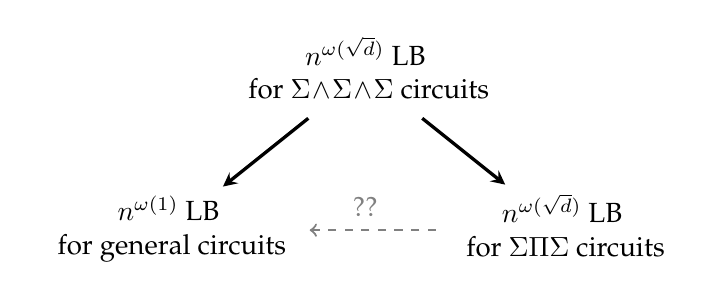
\begin{tikzpicture}
\node (SESES) at (0,0) {$\begin{array}{c}n^{\omega(\sqrt{d})} \text{ LB} \\\text{ for } \SESES \text{ circuits}\end{array}$};
\node (genCkt) at (-2.5,-2) {$\begin{array}{c} n^{\omega(1)} \text{ LB} \\ \text{ for general circuits} \end{array}$}
edge[stealth-, very thick] (SESES);
\node (SEPS) at (2.5,-2) {$\begin{array}{c} n^{\omega(\sqrt{d})} \text{ LB} \\ \text{ for $\SPS$ circuits} \end{array}$}
edge[stealth-, very thick] (SESES)
edge[->, draw=gray, dashed, thick] (genCkt);
\node[text=gray] at (0,-1.7) {??};
\end{tikzpicture}
\end{center}
\caption{Power of $\SESES$ ckts.}
\label{fig:SESES}
\end{figure}


We now have an interesting situation (Figure~\ref{fig:SESES}). On one hand, Corollary~\ref{cor:pow-genckt} states that a lower bound of $n^{\omega(\sqrt{d})}$ for $\SESES$ circuits would yield a super-polynomial lower bound for general arithmetic circuits. On the other, Lemma~\ref{lem:pow-depth3} states that an $n^{\omega(\sqrt{d})}$ lower bound for $\SESES$ circuits would yield a lower bound of $n^{\omega(\sqrt{d})}$ for depth three circuits. 

Could this just be a coincidence? Or, is it the case that any poly-sized arithmetic circuit can be equivalently expressed as a depth three circuit of size $n^{O(\sqrt{d})}$ over $\Q$? As it turns out, there is indeed a depth reduction to convert any arithmetic circuit to a not-too-large depth three circuit over $\Q$. \\

To complete the picture, it suffices to show that a $\wedge\Sigma\wedge$ circuit can be expressed as a $\Sigma\Pi\Sigma$ circuit. This would automatically imply a reduction from $\SESES$ circuits to $\Sigma\Pi\Sigma$ circuits. The last step of the puzzle is the \emph{duality trick} of \cite{sax08}. 

\begin{lemma}[The Duality Trick \cite{sax08}]\label{lem:duality} There exists univariate polynomials $f_{ij}$'s of degree at most $b$ such that
$$
\inparen{z_1 + \dots + z_s}^b \quad = \quad \sum_{i=1}^{sb+1} f_{i1}(z_1)\dots f_{is}(z_s).
$$
\end{lemma}

It is worth noting that the degree of each term on the RHS is $sb$, whereas the LHS just has degree $b$. This is the place where non-homogeneity is introduced. Applying the above lemma for a $\wedge\Sigma\wedge$ circuit such as $(y_1^a + \dots + y_s^a)^b$ gives

\begin{eqnarray*}
(y_1^a + \dots + y_s^a)^b & = & \sum_{i=1}^{sb+1} \prod_{j=1}^s f_{ij}(y_j^a)\\
 & = & \sum_{i=1}^{sb+1} \prod_{j=1}^s \tilde{f}_{ij}(y_j)
\end{eqnarray*}
where $\tilde{f}_{ij}(y) = f_{ij}(y^a)$. Since each $\tilde{f}_{ij}(y)$ is a univariate polynomial, it can be factorized completely over the $\C$, the field of complex numbers. Hence, if $f_{ij}(y) = \prod_k (y - \zeta_{ijk})$, then we get
\begin{eqnarray*}
(y_1^a + \dots + y_s^a)^b & = & \sum_{i=1}^{sb+1} \prod_{j=1}^s \tilde{f}_{ij}(y_j)\\
&= & \sum_{i=1}^{sb+1} \prod_{j=1}^s \prod_{k=1}^b (y_j - \zeta_{ijk})\\
\end{eqnarray*}
which is a depth three circuit! Thus, $(y_1^a + \dots + y_s^a)$ can be expressed as a depth three circuit of size $\poly(s,a,b)$ over $\C$. With a little more effort, one can construct a depth three circuit over $\Q$ as well. Summarizing this is a lemma, we have the following. 

\begin{lemma}
Any $n$-variate degree $d$ polynomial $f$ computed by a homogeneous $\SESES$ of size $s$ over a characteristic zero field $\F$ can also be computed by a depth three circuit of size $\poly(s,n,d)$ over $\F$. 
\end{lemma}

Combining with Corollary~\ref{cor:pow-genckt} and Theorem~\ref{thm:av}, we obtain the main result of \cite{gkks13b}. \\

{\bf Theorem~\ref{thm:chasm-at-3} (restated). }{\em 
Let $f$ be an $n$-variate degree $d$ polynomial computed by an arithmetic circuit of size $s$ over any characteristic zero field. Then there is a $\SPS$ circuit of size $s' \leq s^{O(\sqrt{d})}$ that computes $f$. 
}\\

{\bf Remark. } Note that if we were to start with a degree $d$ polynomial $f$ and apply the above depth reduction, all the linear polynomials that we obtain at bottom are essentially from the application of Fischer's identity on the bottom $\Pi$ layer of fanin $\sqrt{d}$ of the $\SPSPfanin{O(\sqrt{d})}{\sqrt{d}}$ circuit. Hence, the each of the linear polynomials that appear in the final $\SPS$ circuit depend on at most $\sqrt{d}$ variables. In other words, the above Theorem yields a reduction to $\SPS^{[\sqrt{d}]}$ circuits. 

\subsection{Lower bounds for $\SPS$ circuits with small bottom fan-in}

Now let us focus on $\SPS^{[r]}$ circuits, where all linear polynomials in the circuit depend on at most $r$ variables. The following is the key observation of \cite{KayalSaha14} and can be verified easily. 

\begin{observation}[\cite{KayalSaha14}]
Starting with a $\SPS^{[r]}$ circuit $C$ of size $s$ computing a homogeneous $n$-variate polynomial of degree $d$, the resulting $\Sigma\Pi\Sigma\!\wedge\!\Sigma$ circuit $C'$ obtained from Corollary~\ref{cor:d3-d5} is in fact a 
$\Sigma\Pi\Sigma\!\wedge\!\Sigma^{[r]}$ circuit of size $s' = \poly(ns) \cdot 2^{O(\sqrt{d})}$. 

Thus, by expanding the all powers of linear polynomials computed in the bottom two layers of the $\Sigma\Pi\Sigma\!\wedge\!\Sigma$ circuit $C'$, the circuit $C'$ can be rewritten as a homogeneous depth $4$ circuit of bottom support bounded by $r$ and  size $s'' = s' \cdot d^r$
\end{observation}

This observation in combination with Theorem~\ref{thm:KLSS-lowsupp} immediately yields the main theorem of \cite{KayalSaha14}. 

\begin{theorem}[\cite{KayalSaha14}]\label{thm:kaysaha-main}
Over any characteristic zero field $\F$, any $\SPS^{[r]}$ circuit $C$ computing the polynomial $\IMM_{n,d}$, for suitably chosen parameters $n$ and $d$ with $n = d^{O(1)}$, must have size $s = n^{\Omega(d/r)}$. 
\end{theorem}

\subsection{Extensions to low-bottom-fanin depth $5$ circuits}

\cite{KayalSaha14} also prove lower bounds for depth $5$ circuits where the bottom fan-in is bounded. The result proceeds by analysing the random restriction process carefully to decompose any $\Sigma\Pi\Sigma\Pi\Sigma^{[\tau]}$ circuit into a $\Sigma\Pi\Sigma\Pi^{[\sqrt{d}]}$ circuit and another circuit $C'$ such that $\Gamma_{k,\ell}^{[\mathrm{PSD}]}(C') = 0$. We just state their theorem here without proof. 

\begin{theorem}\label{thm:kaysaha-d5}
Let $\F$ be a field of characteristic zero, and let $0\leq \mu < 1$. If $\alpha  = \frac{2\mu + 1}{1 - \mu}$ and $\tau = O(N^\mu)$, then there is a family of $n$-variate degree $d$ polynomials $\inbrace{f_n}$ in $\VNP$ with $n\in [d^{2+\alpha}, 2d^{2+\alpha}]$ such that any homogeneous $\Sigma\Pi\Sigma\Pi\Sigma^{[\tau]}$ circuit computing this polynomial requires size $n^{\Omega(\sqrt{d})}$. 
\end{theorem}

\section{Speculation about lower bounds for homogeneous formulas}\label{sec:hom-formulas}

In this section, we shall look at a possible approach to proving an $n^{\Omega(\log n)}$ lower bound for homogeneous formulas. It is conceivable that variants of the dimension of shifted partial derivatives would be able to give such a lower bound. We will not be presenting any candidate measures, but would instead present a normal form that could perhaps be useful. 

\subsection{A stronger(?) depth reduction for homogeneous formulas}

If we were to prove a lower bound for homogeneous formulas via a depth reduction to $\SPSPfanin{O(\sqrt{d})}{\sqrt{d}}$ circuits, the first step would be to answer the following question:
\begin{quote}
Suppose we apply Theorem~\ref{thm:av} to a polynomial sized circuit $C$ to obtain a $\SPSPfanin{O(\sqrt{d})}{\sqrt{d}}$ circuit $C'$, and also apply Theorem~\ref{thm:av} to a polynomial sized homogeneous formulas $\tilde{C}$ to obtain a $\SPSPfanin{O(\sqrt{d})}{\sqrt{d}}$ circuit $\tilde{C}'$, how is $\tilde{C}'$ structurally different from $C'$?
\end{quote}
Unless we are able to find a non-trivial structural difference between $\tilde{C}'$ and $C'$, it does not make sense to attempt proving lower bounds for homogeneous formulas via $\SPSPfanin{O(\sqrt{d})}{\sqrt{d}}$ circuits. The original proof of \cite{Tav13} of Theorem~\ref{thm:av} does not seem to suggest any structural difference between the two. However, the alternate proof described in Section~\ref{sec:depth-red} allows one to understand this difference better. \\

Recall how the alternate proof proceeded. If $g$ is the polynomial computed by any gate in the circuit $C$ of size $s$, then $g$ can be written as
\[
g\spaced{=} \sum_{i=1}^{\poly(s)} g_{i1} \cdot g_{i2} \cdot g_{i3} \cdot g_{i4} \cdot g_{i5}
\]
where $\sum_j \deg(g_{ij}) = \deg(g)$ for all $i$ and $\deg(g_{ij})\leq \deg(g)/2$. Further $g_{ij}$s are polynomials computed by the children/grandchildren of $g$. With an equation as above, we could recursively keep expanding the larger degree $g_{ij}$'s to eventually get all degrees to be less than $\sqrt{d}$. 

For homogeneous formulas, we can start with a slightly more structured equation instead of the one above. This more structured decomposition was first observed by \cite{HY11a}.  

\begin{lemma}[\cite{HY11a}]\label{lem:HY}
Let $\Phi$ be a homogeneous formula of size $s$. If $f$ is a polynomial computed at an arbitrary gate of $f$, then $f$ can be written as
\begin{equation}\label{eqn:vsbr-hom-form}
f \spaced{=} \sum_{i=1}^s f_{i1} \cdot f_{i2} \cdot \dots \cdot  f_{i\ell}
\end{equation}
where 
\begin{itemize}
\item Each $f_{ij}$ is computable by a homogeneous formula of size at most $s$
\item $\sum_j \deg(f_{ij}) = \deg(f)$ for all $i$
\item $\inparen{\frac{1}{3}}^i \deg(f) \leq \deg(f_{ij}) \leq \inparen{\frac{2}{3}}^i \deg(f)$ for all $i,j$. 
\item $\deg(f_{i\ell}) = 1$ for all $i$. 
\end{itemize}
\end{lemma}
\begin{proof}
Assume that the $\Phi$ is a formula of fan-in $2$ at each gate. This would only increase the depth by a polynomial factor. Starting from the root, walk down the tree by always picking the child of largest degree until we hit a node $v$ of degree at most $\frac{2\deg(f)}{3}$ for the first time. Since the path always picked the child of largest degree, we must have that 
\[
\frac{\deg(f)}{3}\spaced{\leq}\deg(v)\spaced{\leq} \frac{2\deg(f)}{3}
\]
Let $\Phi_v$ denote the sub-formula rooted at $v$, and let $\Phi_{v=0}$ refer to the formula obtained from $\Phi$ by replacing the sub-tree rooted at $v$ by $0$. Let $s_1$ and $s_2$ be the size of $\Phi_v$ and $\Phi_{v=0}$ respectively. (We shall abuse notation and also use $\Phi_v$ and $\Phi_{v=0}$ to refer to the polynomial computed by these formulas.) Then,
\[
f \spaced{=} \Phi_v \cdot A \spaced{+} \Phi_{v=0}
\] 
for some polynomial $A$. Note that homogeneity implies that $\deg(A) + \deg(\Phi_v) = \deg(f)$ and hence $\frac{\deg(f)}{3} \leq \deg(A) \leq \frac{2\deg(f)}{3}$. ($A$ is going to play the role of $f_{i1}$ for some of the $i$'s.)

Observe that the formulas $\Phi_v$ and $\Phi_{v=0}$ `partition' the formula $\Phi$ and hence $s_1 + s_2 \leq s$. By induction on these smaller formulas, we can write
\begin{eqnarray*}
\Phi_v & = & \sum_{i=1}^{s_1} g_{i1} \cdots g_{i\ell}\\
\Phi_{v=0} & = & \sum_{i=1}^{s_2} h_{i1} \cdots h_{i\ell}
\end{eqnarray*}
satisfying the necessary conditions. Since $\frac{\deg(f)}{3} \leq \deg(\Phi_v)\leq \frac{2\deg(f)}{3}$, we have that
\[
f \spaced{=} \sum_{i=1}^{s_1} A \cdot g_{i1} \cdots g_{i\ell} \spaced{+} \sum_{i=1}^{s_2} h_{i1} \cdots h_{i\ell}
\]
satisfies all the degree conditions with $A$ as claimed. To complete the proof, it suffices to show that $A$ can be computed by a homogeneous formula of size $s$. Indeed, the polynomial $A$ is just the product of all siblings of multiplication gates encountered in the path from $v$ to the root. Since each of the siblings are disjoint sub-formulas of $\Phi$, the polynomial $A$ is computable by a homogeneous formula of size at most $s$. 
\end{proof}

With equation~\eqref{eqn:vsbr-hom-form} instead, we can repeat the strategy we used to prove Theorem~\ref{thm:av}. 
\begin{mdframed}
\begin{quote}
Start with (\ref{eqn:vsbr-hom-form}) for the root of the homogeneous formula. 

For each summand $f_{i1}\dots f_{ir}$ in the RHS, if the largest degree $f_{ij}$ has degree more than $\sqrt{d}$, expand that $f_{ij}$ with the its corresponding representation using Lemma~\ref{lem:HY}. 

Repeat this process until all $f_{ij}$'s on the RHS have degree at most $\sqrt{d}$. 
\end{quote}
\end{mdframed}

Again, in the expansion of $f$ of degree $d$ via Lemma~\ref{lem:HY}, every term on the LHS has at least two factors of degree more than $d/9$. The same proof would then yield a $\Sigma\Pi\Sigma\Pi^{[\sqrt{d}]}$ circuit of top fan-in at most $s^{O(\sqrt{d})}$. Did we gain anything with this? We certainly did -- observe that every expansion via Lemma~\ref{lem:HY} yields $O(\log d)$ more factors in each term. In the case of Theorem~\ref{thm:av}, we gained only constantly many factors at each term. Thus, in the resulting depth $4$ circuit has the form
\[
f \spaced{=} \sum_{i=1}^{s^{O(\sqrt{d})}} Q_{i1} \dots Q_{ir}\spaced{,}\text{where $1\leq \deg(Q_{ij})\leq \sqrt{d}$}
\]
and, most importantly, $r = O(\sqrt{d}\log d)$ as opposed to $O(\sqrt{d})$ in the case of Theorem~\ref{thm:av}. This seems to be a key structural difference between depth $4$ circuits obtained from homogeneous formulas as opposed to depth $4$ circuits obtained from general arithmetic circuits! We summarize this below. 

\begin{theorem}
If $f$ is an $n$-variate degree $d$ polynomial computed by a homogeneous formula of size $s$, then there is a homogeneous $\SPSPfanin{O(\sqrt{d}\log d)}{\sqrt{d}}$ circuit computing $f$ with top fanin at most $s^{O(\sqrt{d})}$. 
\end{theorem}

\subsubsection*{Is this useful?}

It is not clear if the above structural difference can be exploited to give a complexity measure. But it is very much possible that the some small modification of measure of dimension of shifted partials derivatives might be a measure that works. The reason we believe that is because the results of \cite{gkks13,KSS13,KS14a} give explicit $n$-variate degree $d$ polynomials that admit a top fan-in lower bound of $n^{\Omega(d/t)}$ for depth $4$ circuits with \emph{maximum bottom degree} bounded by $t$. \\

{\bf Question. }Could that be changed to give an $n^{\Omega(d/t)}$ lower bound for depth $4$ circuits with \emph{average bottom degree} bounded by $t$? \\

If this were true, then we obtain an $n^{\Omega(\log d)}$ lower bound for the size of homogeneous formulas computing an explicit $n$-variate degree $d$ polynomial. Also, we need to keep in mind that any circuit of polynomial size has an equivalent homogeneous formula of size $n^{O(\log d)}$. Hence, if we are hoping to come up with a method that might prove a lower bound for homogeneous formulas but not for general circuits, then method should not be able to yield a lower bound better than $n^{\Omega(\log d)}$. This indeed seems to be the case in this approach. Maybe this is the right depth reduction to work with to prove lower bounds for homogeneous formulas, maybe not. Either way, we shall probably find out soon enough!

\section{Conclusion}\label{sec:conc}

Quite a lot seems to be happening lately in arithmetic circuits. The last few results were on $n^{\Omega(\sqrt{d})}$ lower bounds for homogeneous depth $4$, non-homogeneous depth $3$ circuits with small bottom fanin, and homogeneous depth $5$ with small bottom fanin. Perhaps in the near future, we would be able to obtain $n^{\Omega(\sqrt{d})}$ lower bounds for non-homogeneous depth $3$ or homogeneous depth $5$ circuits without any bottom fanin restrictions. These are all interesting problems to work on, and should be very much within reach of current techniques. However, it is to be noted that if we wish to separate $\VP$ and $\VNP$, we need to break past $n^{\Omega(\sqrt{d})}$. It appears (at least to us) this task would require very different techniques and seems unlikely that small variants of shifted partial derivatives might just get us past $n^{\Omega(\sqrt{d})}$. Nevertheless, Open Problem~\ref{openprob:main} presents a concrete and extremely simple looking model to work with, for which we need to prove an $n^{\omega(\sqrt{d})}$ lower bound to separate $\VP$ and $\VNP$. We conclude by stating the problem again to emphasize the point. 

\begin{mdframed}
{\bf Open Problem. } {\em Find an explicit $n$-variate degree $d$ polynomial $f$ such that any expression of the form
\[
f \quad=\quad (Q_1)^{\sqrt{d}} + \dots + (Q_{s})^{\sqrt{d}}\quad,\quad \deg(Q_i) \leq \sqrt{d} \text{ for all $i$}
\]
must have $s = n^{\omega(\sqrt{d})}$. }
\end{mdframed}


\bibliographystyle{alpha}
\bibliography{references}

\end{document}



\bibliographystyle{alpha}
\bibliography{references}


\end{document}

